\documentclass[twoside]{book}

% Packages required by doxygen
\usepackage{fixltx2e}
\usepackage{calc}
\usepackage{doxygen}
\usepackage[export]{adjustbox} % also loads graphicx
\usepackage{graphicx}
\usepackage[utf8]{inputenc}
\usepackage{makeidx}
\usepackage{multicol}
\usepackage{multirow}
\PassOptionsToPackage{warn}{textcomp}
\usepackage{textcomp}
\usepackage[nointegrals]{wasysym}
\usepackage[table]{xcolor}

% Font selection
\usepackage[T1]{fontenc}
\usepackage[scaled=.90]{helvet}
\usepackage{courier}
\usepackage{amssymb}
\usepackage{sectsty}
\renewcommand{\familydefault}{\sfdefault}
\allsectionsfont{%
  \fontseries{bc}\selectfont%
  \color{darkgray}%
}
\renewcommand{\DoxyLabelFont}{%
  \fontseries{bc}\selectfont%
  \color{darkgray}%
}
\newcommand{\+}{\discretionary{\mbox{\scriptsize$\hookleftarrow$}}{}{}}

% Page & text layout
\usepackage{geometry}
\geometry{%
  a4paper,%
  top=2.5cm,%
  bottom=2.5cm,%
  left=2.5cm,%
  right=2.5cm%
}
\tolerance=750
\hfuzz=15pt
\hbadness=750
\setlength{\emergencystretch}{15pt}
\setlength{\parindent}{0cm}
\setlength{\parskip}{3ex plus 2ex minus 2ex}
\makeatletter
\renewcommand{\paragraph}{%
  \@startsection{paragraph}{4}{0ex}{-1.0ex}{1.0ex}{%
    \normalfont\normalsize\bfseries\SS@parafont%
  }%
}
\renewcommand{\subparagraph}{%
  \@startsection{subparagraph}{5}{0ex}{-1.0ex}{1.0ex}{%
    \normalfont\normalsize\bfseries\SS@subparafont%
  }%
}
\makeatother

% Headers & footers
\usepackage{fancyhdr}
\pagestyle{fancyplain}
\fancyhead[LE]{\fancyplain{}{\bfseries\thepage}}
\fancyhead[CE]{\fancyplain{}{}}
\fancyhead[RE]{\fancyplain{}{\bfseries\leftmark}}
\fancyhead[LO]{\fancyplain{}{\bfseries\rightmark}}
\fancyhead[CO]{\fancyplain{}{}}
\fancyhead[RO]{\fancyplain{}{\bfseries\thepage}}
\fancyfoot[LE]{\fancyplain{}{}}
\fancyfoot[CE]{\fancyplain{}{}}
\fancyfoot[RE]{\fancyplain{}{\bfseries\scriptsize Generated by Doxygen }}
\fancyfoot[LO]{\fancyplain{}{\bfseries\scriptsize Generated by Doxygen }}
\fancyfoot[CO]{\fancyplain{}{}}
\fancyfoot[RO]{\fancyplain{}{}}
\renewcommand{\footrulewidth}{0.4pt}
\renewcommand{\chaptermark}[1]{%
  \markboth{#1}{}%
}
\renewcommand{\sectionmark}[1]{%
  \markright{\thesection\ #1}%
}

% Indices & bibliography
\usepackage{natbib}
\usepackage[titles]{tocloft}
\setcounter{tocdepth}{3}
\setcounter{secnumdepth}{5}
\makeindex

% Hyperlinks (required, but should be loaded last)
\usepackage{ifpdf}
\ifpdf
  \usepackage[pdftex,pagebackref=true]{hyperref}
\else
  \usepackage[ps2pdf,pagebackref=true]{hyperref}
\fi
\hypersetup{%
  colorlinks=true,%
  linkcolor=blue,%
  citecolor=blue,%
  unicode%
}

% Custom commands
\newcommand{\clearemptydoublepage}{%
  \newpage{\pagestyle{empty}\cleardoublepage}%
}

\usepackage{caption}
\captionsetup{labelsep=space,justification=centering,font={bf},singlelinecheck=off,skip=4pt,position=top}

%===== C O N T E N T S =====

\begin{document}

% Titlepage & ToC
\hypersetup{pageanchor=false,
             bookmarksnumbered=true,
             pdfencoding=unicode
            }
\pagenumbering{roman}
\begin{titlepage}
\vspace*{7cm}
\begin{center}%
{\Large alibvr }\\
\vspace*{1cm}
{\large Generated by Doxygen 1.8.11}\\
\end{center}
\end{titlepage}
\clearemptydoublepage
\tableofcontents
\clearemptydoublepage
\pagenumbering{arabic}
\hypersetup{pageanchor=true}

%--- Begin generated contents ---
\chapter{Module Index}
\section{Modules}
Here is a list of all modules\+:\begin{DoxyCompactList}
\item \contentsline{section}{$<$avr/io.h$>$\+: A\+VR device-\/specific IO definitions}{\pageref{group__avr__io}}{}
\end{DoxyCompactList}

\chapter{Namespace Index}
\section{Namespace List}
Here is a list of all documented namespaces with brief descriptions\+:\begin{DoxyCompactList}
\item\contentsline{section}{\hyperlink{namespace__pulse__uart}{\+\_\+pulse\+\_\+uart} }{\pageref{namespace__pulse__uart}}{}
\item\contentsline{section}{\hyperlink{namespaceadc}{adc} }{\pageref{namespaceadc}}{}
\item\contentsline{section}{\hyperlink{namespaceadc_1_1Input}{adc\+::\+Input} \\*In addition to the A\+D\+C-\/pins the adc subsystem can also use an internal temperature sensor, an internal 1.\+1V reference voltage and ground as input for a conversion }{\pageref{namespaceadc_1_1Input}}{}
\item\contentsline{section}{\hyperlink{namespaceclock}{clock} \\*This file uses {\ttfamily Timer0} to provide a system clock }{\pageref{namespaceclock}}{}
\item\contentsline{section}{\hyperlink{namespaceports}{ports} \\*Avr Atmegas access and control pins through registers. The registers are 8 bit wide and up to 8 pins are therefore controlled with every register }{\pageref{namespaceports}}{}
\end{DoxyCompactList}

\chapter{Hierarchical Index}
\section{Class Hierarchy}
This inheritance list is sorted roughly, but not completely, alphabetically\+:\begin{DoxyCompactList}
\item \contentsline{section}{\+\_\+twi\+:\+:\+\_\+\+Bit\+Rate\+Config}{\pageref{struct__twi_1_1__BitRateConfig}}{}
\item \contentsline{section}{clock\+:\+:\+\_\+\+Clock}{\pageref{classclock_1_1__Clock}}{}
\item \contentsline{section}{ports\+:\+:\+\_\+\+Io$<$ p, b, io $>$}{\pageref{structports_1_1__Io}}{}
\item \contentsline{section}{adc\+:\+:Adc$<$ Default\+Ref, Default\+Input, Default\+Mode, Task, Default\+Global\+Irq $>$}{\pageref{classadc_1_1Adc}}{}
\item \contentsline{section}{bits16\+\_\+hilo\+\_\+s}{\pageref{structbits16__hilo__s}}{}
\item \contentsline{section}{bits16\+\_\+lohi\+\_\+s}{\pageref{structbits16__lohi__s}}{}
\item \contentsline{section}{bits16\+\_\+s}{\pageref{unionbits16__s}}{}
\item \contentsline{section}{bits32\+\_\+hilo\+\_\+s}{\pageref{structbits32__hilo__s}}{}
\item \contentsline{section}{bits32\+\_\+lohi\+\_\+s}{\pageref{structbits32__lohi__s}}{}
\item \contentsline{section}{bits32\+\_\+t}{\pageref{unionbits32__t}}{}
\item \contentsline{section}{bits64\+\_\+hilo\+\_\+s}{\pageref{structbits64__hilo__s}}{}
\item \contentsline{section}{bits64\+\_\+lohi\+\_\+s}{\pageref{structbits64__lohi__s}}{}
\item \contentsline{section}{bits64\+\_\+s}{\pageref{unionbits64__s}}{}
\item \contentsline{section}{Buffer$<$ buffer\+\_\+size, Use\+Markers, Overwrite\+If\+Full $>$}{\pageref{classBuffer}}{}
\item \contentsline{section}{Buffer$<$ 0, Use\+Markers, overwrite\+If\+Full $>$}{\pageref{classBuffer_3_010_00_01UseMarkers_00_01overwriteIfFull_01_4}}{}
\item \contentsline{section}{Buttons$<$ Button\+List $>$}{\pageref{classButtons}}{}
\item \contentsline{section}{\+\_\+transmission\+:\+:Clear\+Errors}{\pageref{class__transmission_1_1ClearErrors}}{}
\item \contentsline{section}{std\+:\+:conditional$<$ B, T, F $>$}{\pageref{structstd_1_1conditional}}{}
\item \contentsline{section}{std\+:\+:conditional$<$ false, T, F $>$}{\pageref{structstd_1_1conditional_3_01false_00_01T_00_01F_01_4}}{}
\item \contentsline{section}{\+\_\+twi\+:\+:Data\+Provider\+Task}{\pageref{class__twi_1_1DataProviderTask}}{}
\item \contentsline{section}{\+\_\+spi\+:\+:Data\+Provider\+Task}{\pageref{class__spi_1_1DataProviderTask}}{}
\item \contentsline{section}{\+\_\+pulse\+\_\+uart\+:\+:Do\+Nothing}{\pageref{class__pulse__uart_1_1DoNothing}}{}
\item \contentsline{section}{\+\_\+uart\+:\+:Do\+Nothing}{\pageref{class__uart_1_1DoNothing}}{}
\item \contentsline{section}{\+\_\+spi\+:\+:Do\+Nothing}{\pageref{class__spi_1_1DoNothing}}{}
\item \contentsline{section}{\+\_\+timer\+:\+:Do\+Nothing}{\pageref{struct__timer_1_1DoNothing}}{}
\item \contentsline{section}{\+\_\+twi\+:\+:Do\+Nothing}{\pageref{class__twi_1_1DoNothing}}{}
\item \contentsline{section}{\+\_\+buttons\+:\+:Do\+Nothing\+Matrix\+Listener}{\pageref{struct__buttons_1_1DoNothingMatrixListener}}{}
\item \contentsline{section}{adc\+:\+:Input\+:\+:Gnd}{\pageref{structadc_1_1Input_1_1Gnd}}{}
\item \contentsline{section}{std\+:\+:integral\+\_\+constant$<$ T, v $>$}{\pageref{structstd_1_1integral__constant}}{}
\begin{DoxyCompactList}
\item \contentsline{section}{std\+:\+:is\+\_\+same$<$ T, U $>$}{\pageref{structstd_1_1is__same}}{}
\item \contentsline{section}{std\+:\+:is\+\_\+same$<$ T, T $>$}{\pageref{structstd_1_1is__same_3_01T_00_01T_01_4}}{}
\end{DoxyCompactList}
\item \contentsline{section}{Lcd$<$ L\+C\+D\+\_\+\+D7, L\+C\+D\+\_\+\+D6, L\+C\+D\+\_\+\+D5, L\+C\+D\+\_\+\+D4, L\+C\+D\+\_\+\+E\+N\+A\+B\+LE, L\+C\+D\+\_\+\+R\+E\+G\+\_\+\+S\+E\+L\+E\+CT $>$}{\pageref{classLcd}}{}
\item \contentsline{section}{Matrix\+Buttons$<$ Row\+List, Column\+List, Listener $>$}{\pageref{classMatrixButtons}}{}
\item \contentsline{section}{Modbus$<$ address\+Id, Modbus\+Data\+List, Connection\+Ctrl $>$}{\pageref{classModbus}}{}
\item \contentsline{section}{\+\_\+timer0\+:\+:Mode\+Support$<$ Mode, Clock\+Select $>$}{\pageref{struct__timer0_1_1ModeSupport}}{}
\item \contentsline{section}{\+\_\+spi\+:\+:No\+SS}{\pageref{class__spi_1_1NoSS}}{}
\item \contentsline{section}{std\+:\+:numeric\+\_\+limits$<$ T $>$}{\pageref{classstd_1_1numeric__limits}}{}
\item \contentsline{section}{std\+:\+:numeric\+\_\+limits$<$ uint16\+\_\+t $>$}{\pageref{classstd_1_1numeric__limits_3_01uint16__t_01_4}}{}
\item \contentsline{section}{std\+:\+:numeric\+\_\+limits$<$ uint8\+\_\+t $>$}{\pageref{classstd_1_1numeric__limits_3_01uint8__t_01_4}}{}
\item \contentsline{section}{Pgm\+Data\+Ptr$<$ T $>$}{\pageref{classPgmDataPtr}}{}
\item \contentsline{section}{ports\+:\+:Pin$<$ p, b $>$}{\pageref{structports_1_1Pin}}{}
\item \contentsline{section}{\+\_\+buttons\+:\+:Pin\+List$<$ Pins $>$}{\pageref{class__buttons_1_1PinList}}{}
\item \contentsline{section}{Pulse\+Uart\+Tx$<$ Tx\+Pin, zero\+Bit\+Duration, \+\_\+tx\+\_\+buffer\+\_\+size, Task, one\+Bit\+Duration, sync\+Bit\+Duration, inverse\+Output $>$}{\pageref{classPulseUartTx}}{}
\item \contentsline{section}{Pwm$<$ TimerN, Mode, Out\+ModeA, Out\+ModeB, Set\+D\+D\+R\+\_\+A, Set\+D\+D\+R\+\_\+B, TaskA, TaskB, Task\+OvF $>$}{\pageref{classPwm}}{}
\item \contentsline{section}{Serial\+Modbus$<$ address\+Id, Modbus\+Data\+List, baud, stop\+\_\+bits, parity\+\_\+bit, data\+\_\+bits, baud\+\_\+tol $>$}{\pageref{classSerialModbus}}{}
\item \contentsline{section}{\+\_\+servo\+:\+:Servo\+Pause$<$ Pause\+Length $>$}{\pageref{class__servo_1_1ServoPause}}{}
\item \contentsline{section}{Servos$<$ Servo\+List $>$}{\pageref{classServos}}{}
\item \contentsline{section}{Spi\+Async$<$ Clock\+Select, Mode, tx\+\_\+buffer\+\_\+size, rx\+\_\+buffer\+\_\+size, Irq\+Task, default\+\_\+char, \+\_\+\+SS, Data\+Order, Data\+Mode $>$}{\pageref{classSpiAsync}}{}
\item \contentsline{section}{Spi\+Master$<$ Clock\+Select, tx\+\_\+buffer\+\_\+size, rx\+\_\+buffer\+\_\+size, Irq\+Task, SS, Data\+Order, Data\+Mode $>$}{\pageref{classSpiMaster}}{}
\item \contentsline{section}{Spi\+Slave$<$ tx\+\_\+buffer\+\_\+size, rx\+\_\+buffer\+\_\+size, Irq\+Task, default\+\_\+char, Data\+Order, Data\+Mode $>$}{\pageref{classSpiSlave}}{}
\item \contentsline{section}{Spi\+Sync$<$ Clock\+Select, Mode, \+\_\+\+SS, Data\+Order, Data\+Mode $>$}{\pageref{classSpiSync}}{}
\item \contentsline{section}{Static\+\_\+\+Buffer$<$ buffer\+\_\+size, unique\+\_\+id, Use\+Markers, Overwrite\+If\+Full $>$}{\pageref{classStatic__Buffer}}{}
\item \contentsline{section}{adc\+:\+:Input\+:\+:Temperature}{\pageref{structadc_1_1Input_1_1Temperature}}{}
\item \contentsline{section}{\+\_\+timer\+:\+:Timer0}{\pageref{struct__timer_1_1Timer0}}{}
\item \contentsline{section}{\+\_\+timer2\+:\+:Timer\+Def}{\pageref{struct__timer2_1_1TimerDef}}{}
\item \contentsline{section}{\+\_\+timer1\+:\+:Timer\+Def}{\pageref{struct__timer1_1_1TimerDef}}{}
\item \contentsline{section}{\+\_\+timer0\+:\+:Timer\+Def}{\pageref{struct__timer0_1_1TimerDef}}{}
\item \contentsline{section}{Twi\+Master$<$ tx\+\_\+buffer\+\_\+size, rx\+\_\+buffer\+\_\+size, Irq\+Task, address, general\+Call, max\+Speed, pull\+\_\+up $>$}{\pageref{classTwiMaster}}{}
\item \contentsline{section}{Uart$<$ baud, \+\_\+tx\+\_\+buffer\+\_\+size, \+\_\+rx\+\_\+buffer\+\_\+size, use\+\_\+irqs, Irq\+Task, stop\+\_\+bits, parity\+\_\+bit, data\+\_\+bits, baud\+\_\+tol $>$}{\pageref{classUart}}{}
\item \contentsline{section}{adc\+:\+:Input\+:\+:Unset}{\pageref{structadc_1_1Input_1_1Unset}}{}
\item \contentsline{section}{adc\+:\+:Input\+:\+:V1\+\_\+1}{\pageref{structadc_1_1Input_1_1V1__1}}{}
\end{DoxyCompactList}

\chapter{Class Index}
\section{Class List}
Here are the classes, structs, unions and interfaces with brief descriptions\+:\begin{DoxyCompactList}
\item\contentsline{section}{\hyperlink{struct__twi_1_1__BitRateConfig}{\+\_\+twi\+::\+\_\+\+Bit\+Rate\+Config} }{\pageref{struct__twi_1_1__BitRateConfig}}{}
\item\contentsline{section}{\hyperlink{classclock_1_1__Clock}{clock\+::\+\_\+\+Clock} \\*Initialization code and access to the \+\_\+clock variable }{\pageref{classclock_1_1__Clock}}{}
\item\contentsline{section}{\hyperlink{structports_1_1__Io}{ports\+::\+\_\+\+Io$<$ p, b, io $>$} \\*This class implements the cast operations from uint8\+\_\+t and the typesafe enums\+: Data\+Direction and Pull\+Up }{\pageref{structports_1_1__Io}}{}
\item\contentsline{section}{\hyperlink{classadc_1_1Adc}{adc\+::\+Adc$<$ Default\+Ref, Default\+Input, Default\+Mode, Task, Default\+Global\+Irq $>$} \\*Static functions for initialization, adc controls and irqs }{\pageref{classadc_1_1Adc}}{}
\item\contentsline{section}{\hyperlink{structbits16__hilo__s}{bits16\+\_\+hilo\+\_\+s} \\*This file contains {\ttfamily typedef}s which make it easier to access specific bytes of multi-\/byte values }{\pageref{structbits16__hilo__s}}{}
\item\contentsline{section}{\hyperlink{structbits16__lohi__s}{bits16\+\_\+lohi\+\_\+s} }{\pageref{structbits16__lohi__s}}{}
\item\contentsline{section}{\hyperlink{unionbits16__s}{bits16\+\_\+s} }{\pageref{unionbits16__s}}{}
\item\contentsline{section}{\hyperlink{structbits32__hilo__s}{bits32\+\_\+hilo\+\_\+s} }{\pageref{structbits32__hilo__s}}{}
\item\contentsline{section}{\hyperlink{structbits32__lohi__s}{bits32\+\_\+lohi\+\_\+s} }{\pageref{structbits32__lohi__s}}{}
\item\contentsline{section}{\hyperlink{unionbits32__t}{bits32\+\_\+t} }{\pageref{unionbits32__t}}{}
\item\contentsline{section}{\hyperlink{structbits64__hilo__s}{bits64\+\_\+hilo\+\_\+s} }{\pageref{structbits64__hilo__s}}{}
\item\contentsline{section}{\hyperlink{structbits64__lohi__s}{bits64\+\_\+lohi\+\_\+s} }{\pageref{structbits64__lohi__s}}{}
\item\contentsline{section}{\hyperlink{unionbits64__s}{bits64\+\_\+s} }{\pageref{unionbits64__s}}{}
\item\contentsline{section}{\hyperlink{classBuffer}{Buffer$<$ buffer\+\_\+size, Use\+Markers, Overwrite\+If\+Full $>$} }{\pageref{classBuffer}}{}
\item\contentsline{section}{\hyperlink{classBuffer_3_010_00_01UseMarkers_00_01overwriteIfFull_01_4}{Buffer$<$ 0, Use\+Markers, overwrite\+If\+Full $>$} }{\pageref{classBuffer_3_010_00_01UseMarkers_00_01overwriteIfFull_01_4}}{}
\item\contentsline{section}{\hyperlink{classButtons}{Buttons$<$ Button\+List $>$} }{\pageref{classButtons}}{}
\item\contentsline{section}{\hyperlink{class__transmission_1_1ClearErrors}{\+\_\+transmission\+::\+Clear\+Errors} }{\pageref{class__transmission_1_1ClearErrors}}{}
\item\contentsline{section}{\hyperlink{structstd_1_1conditional}{std\+::conditional$<$ B, T, F $>$} }{\pageref{structstd_1_1conditional}}{}
\item\contentsline{section}{\hyperlink{structstd_1_1conditional_3_01false_00_01T_00_01F_01_4}{std\+::conditional$<$ false, T, F $>$} }{\pageref{structstd_1_1conditional_3_01false_00_01T_00_01F_01_4}}{}
\item\contentsline{section}{\hyperlink{class__twi_1_1DataProviderTask}{\+\_\+twi\+::\+Data\+Provider\+Task} }{\pageref{class__twi_1_1DataProviderTask}}{}
\item\contentsline{section}{\hyperlink{class__spi_1_1DataProviderTask}{\+\_\+spi\+::\+Data\+Provider\+Task} }{\pageref{class__spi_1_1DataProviderTask}}{}
\item\contentsline{section}{\hyperlink{class__pulse__uart_1_1DoNothing}{\+\_\+pulse\+\_\+uart\+::\+Do\+Nothing} }{\pageref{class__pulse__uart_1_1DoNothing}}{}
\item\contentsline{section}{\hyperlink{class__uart_1_1DoNothing}{\+\_\+uart\+::\+Do\+Nothing} }{\pageref{class__uart_1_1DoNothing}}{}
\item\contentsline{section}{\hyperlink{class__spi_1_1DoNothing}{\+\_\+spi\+::\+Do\+Nothing} }{\pageref{class__spi_1_1DoNothing}}{}
\item\contentsline{section}{\hyperlink{struct__timer_1_1DoNothing}{\+\_\+timer\+::\+Do\+Nothing} }{\pageref{struct__timer_1_1DoNothing}}{}
\item\contentsline{section}{\hyperlink{class__twi_1_1DoNothing}{\+\_\+twi\+::\+Do\+Nothing} }{\pageref{class__twi_1_1DoNothing}}{}
\item\contentsline{section}{\hyperlink{struct__buttons_1_1DoNothingMatrixListener}{\+\_\+buttons\+::\+Do\+Nothing\+Matrix\+Listener} }{\pageref{struct__buttons_1_1DoNothingMatrixListener}}{}
\item\contentsline{section}{\hyperlink{structadc_1_1Input_1_1Gnd}{adc\+::\+Input\+::\+Gnd} \\*Ground }{\pageref{structadc_1_1Input_1_1Gnd}}{}
\item\contentsline{section}{\hyperlink{structstd_1_1integral__constant}{std\+::integral\+\_\+constant$<$ T, v $>$} }{\pageref{structstd_1_1integral__constant}}{}
\item\contentsline{section}{\hyperlink{structstd_1_1is__same}{std\+::is\+\_\+same$<$ T, U $>$} }{\pageref{structstd_1_1is__same}}{}
\item\contentsline{section}{\hyperlink{structstd_1_1is__same_3_01T_00_01T_01_4}{std\+::is\+\_\+same$<$ T, T $>$} }{\pageref{structstd_1_1is__same_3_01T_00_01T_01_4}}{}
\item\contentsline{section}{\hyperlink{classLcd}{Lcd$<$ L\+C\+D\+\_\+\+D7, L\+C\+D\+\_\+\+D6, L\+C\+D\+\_\+\+D5, L\+C\+D\+\_\+\+D4, L\+C\+D\+\_\+\+E\+N\+A\+B\+L\+E, L\+C\+D\+\_\+\+R\+E\+G\+\_\+\+S\+E\+L\+E\+C\+T $>$} }{\pageref{classLcd}}{}
\item\contentsline{section}{\hyperlink{classMatrixButtons}{Matrix\+Buttons$<$ Row\+List, Column\+List, Listener $>$} }{\pageref{classMatrixButtons}}{}
\item\contentsline{section}{\hyperlink{classModbus}{Modbus$<$ address\+Id, Modbus\+Data\+List, Connection\+Ctrl $>$} }{\pageref{classModbus}}{}
\item\contentsline{section}{\hyperlink{struct__timer0_1_1ModeSupport}{\+\_\+timer0\+::\+Mode\+Support$<$ Mode, Clock\+Select $>$} }{\pageref{struct__timer0_1_1ModeSupport}}{}
\item\contentsline{section}{\hyperlink{class__spi_1_1NoSS}{\+\_\+spi\+::\+No\+SS} }{\pageref{class__spi_1_1NoSS}}{}
\item\contentsline{section}{\hyperlink{classstd_1_1numeric__limits}{std\+::numeric\+\_\+limits$<$ T $>$} }{\pageref{classstd_1_1numeric__limits}}{}
\item\contentsline{section}{\hyperlink{classstd_1_1numeric__limits_3_01uint16__t_01_4}{std\+::numeric\+\_\+limits$<$ uint16\+\_\+t $>$} }{\pageref{classstd_1_1numeric__limits_3_01uint16__t_01_4}}{}
\item\contentsline{section}{\hyperlink{classstd_1_1numeric__limits_3_01uint8__t_01_4}{std\+::numeric\+\_\+limits$<$ uint8\+\_\+t $>$} }{\pageref{classstd_1_1numeric__limits_3_01uint8__t_01_4}}{}
\item\contentsline{section}{\hyperlink{classPgmDataPtr}{Pgm\+Data\+Ptr$<$ T $>$} }{\pageref{classPgmDataPtr}}{}
\item\contentsline{section}{\hyperlink{structports_1_1Pin}{ports\+::\+Pin$<$ p, b $>$} \\*Every pin of the IC is defined using the template arguments {\ttfamily enum \+\_\+\+Port p} and {\ttfamily uint8\+\_\+t b} using {\ttfamily typedef}s of this class }{\pageref{structports_1_1Pin}}{}
\item\contentsline{section}{\hyperlink{class__buttons_1_1PinList}{\+\_\+buttons\+::\+Pin\+List$<$ Pins $>$} }{\pageref{class__buttons_1_1PinList}}{}
\item\contentsline{section}{\hyperlink{classPulseUartTx}{Pulse\+Uart\+Tx$<$ Tx\+Pin, zero\+Bit\+Duration, \+\_\+tx\+\_\+buffer\+\_\+size, Task, one\+Bit\+Duration, sync\+Bit\+Duration, inverse\+Output $>$} }{\pageref{classPulseUartTx}}{}
\item\contentsline{section}{\hyperlink{classPwm}{Pwm$<$ Timer\+N, Mode, Out\+Mode\+A, Out\+Mode\+B, Set\+D\+D\+R\+\_\+\+A, Set\+D\+D\+R\+\_\+\+B, Task\+A, Task\+B, Task\+Ov\+F $>$} }{\pageref{classPwm}}{}
\item\contentsline{section}{\hyperlink{classSerialModbus}{Serial\+Modbus$<$ address\+Id, Modbus\+Data\+List, baud, stop\+\_\+bits, parity\+\_\+bit, data\+\_\+bits, baud\+\_\+tol $>$} }{\pageref{classSerialModbus}}{}
\item\contentsline{section}{\hyperlink{class__servo_1_1ServoPause}{\+\_\+servo\+::\+Servo\+Pause$<$ Pause\+Length $>$} }{\pageref{class__servo_1_1ServoPause}}{}
\item\contentsline{section}{\hyperlink{classServos}{Servos$<$ Servo\+List $>$} }{\pageref{classServos}}{}
\item\contentsline{section}{\hyperlink{classSpiAsync}{Spi\+Async$<$ Clock\+Select, Mode, tx\+\_\+buffer\+\_\+size, rx\+\_\+buffer\+\_\+size, Irq\+Task, default\+\_\+char, \+\_\+\+S\+S, Data\+Order, Data\+Mode $>$} }{\pageref{classSpiAsync}}{}
\item\contentsline{section}{\hyperlink{classSpiMaster}{Spi\+Master$<$ Clock\+Select, tx\+\_\+buffer\+\_\+size, rx\+\_\+buffer\+\_\+size, Irq\+Task, S\+S, Data\+Order, Data\+Mode $>$} }{\pageref{classSpiMaster}}{}
\item\contentsline{section}{\hyperlink{classSpiSlave}{Spi\+Slave$<$ tx\+\_\+buffer\+\_\+size, rx\+\_\+buffer\+\_\+size, Irq\+Task, default\+\_\+char, Data\+Order, Data\+Mode $>$} }{\pageref{classSpiSlave}}{}
\item\contentsline{section}{\hyperlink{classSpiSync}{Spi\+Sync$<$ Clock\+Select, Mode, \+\_\+\+S\+S, Data\+Order, Data\+Mode $>$} }{\pageref{classSpiSync}}{}
\item\contentsline{section}{\hyperlink{classStatic__Buffer}{Static\+\_\+\+Buffer$<$ buffer\+\_\+size, unique\+\_\+id, Use\+Markers, Overwrite\+If\+Full $>$} }{\pageref{classStatic__Buffer}}{}
\item\contentsline{section}{\hyperlink{structadc_1_1Input_1_1Temperature}{adc\+::\+Input\+::\+Temperature} \\*"The measured voltage has a linear relationship to the temperature \mbox{[}...\mbox{]}. The voltage sensitivity is approximately 1 m\+V/°C and the accuracy of the temperature measurement is +/-\/ 10°C." (Atmega docs) }{\pageref{structadc_1_1Input_1_1Temperature}}{}
\item\contentsline{section}{\hyperlink{struct__timer_1_1Timer0}{\+\_\+timer\+::\+Timer0} }{\pageref{struct__timer_1_1Timer0}}{}
\item\contentsline{section}{\hyperlink{struct__timer2_1_1TimerDef}{\+\_\+timer2\+::\+Timer\+Def} }{\pageref{struct__timer2_1_1TimerDef}}{}
\item\contentsline{section}{\hyperlink{struct__timer1_1_1TimerDef}{\+\_\+timer1\+::\+Timer\+Def} }{\pageref{struct__timer1_1_1TimerDef}}{}
\item\contentsline{section}{\hyperlink{struct__timer0_1_1TimerDef}{\+\_\+timer0\+::\+Timer\+Def} }{\pageref{struct__timer0_1_1TimerDef}}{}
\item\contentsline{section}{\hyperlink{classTwiMaster}{Twi\+Master$<$ tx\+\_\+buffer\+\_\+size, rx\+\_\+buffer\+\_\+size, Irq\+Task, address, general\+Call, max\+Speed, pull\+\_\+up $>$} }{\pageref{classTwiMaster}}{}
\item\contentsline{section}{\hyperlink{classUart}{Uart$<$ baud, \+\_\+tx\+\_\+buffer\+\_\+size, \+\_\+rx\+\_\+buffer\+\_\+size, use\+\_\+irqs, Irq\+Task, stop\+\_\+bits, parity\+\_\+bit, data\+\_\+bits, baud\+\_\+tol $>$} }{\pageref{classUart}}{}
\item\contentsline{section}{\hyperlink{structadc_1_1Input_1_1Unset}{adc\+::\+Input\+::\+Unset} \\*Use \hyperlink{structadc_1_1Input_1_1Unset}{Unset} during initialization if you intend to use different inputs. Using \hyperlink{structadc_1_1Input_1_1Unset}{Unset} doesn\textquotesingle{}t prevent you from using different inputs, but maybe makes your intentations clearer }{\pageref{structadc_1_1Input_1_1Unset}}{}
\item\contentsline{section}{\hyperlink{structadc_1_1Input_1_1V1__1}{adc\+::\+Input\+::\+V1\+\_\+1} \\*The internal 1.\+1V bandgap reference voltage }{\pageref{structadc_1_1Input_1_1V1__1}}{}
\end{DoxyCompactList}

\chapter{File Index}
\section{File List}
Here is a list of all documented files with brief descriptions\+:\begin{DoxyCompactList}
\item\contentsline{section}{src/{\bfseries adc.\+h} }{\pageref{d7/d19/adc_8h}}{}
\item\contentsline{section}{src/{\bfseries buffer.\+h} }{\pageref{d5/d08/buffer_8h}}{}
\item\contentsline{section}{src/{\bfseries buttons.\+h} }{\pageref{de/d05/buttons_8h}}{}
\item\contentsline{section}{src/{\bfseries bytes.\+h} }{\pageref{df/dd9/bytes_8h}}{}
\item\contentsline{section}{src/{\bfseries clock.\+h} }{\pageref{d7/d6e/clock_8h}}{}
\item\contentsline{section}{src/{\bfseries clock\+\_\+select.\+h} }{\pageref{d1/d46/clock__select_8h}}{}
\item\contentsline{section}{src/{\bfseries cmacros.\+h} }{\pageref{db/df6/cmacros_8h}}{}
\item\contentsline{section}{src/{\bfseries io.\+h} }{\pageref{dc/dac/io_8h}}{}
\item\contentsline{section}{src/{\bfseries irqs.\+h} }{\pageref{df/dc7/irqs_8h}}{}
\item\contentsline{section}{src/{\bfseries lcd.\+h} }{\pageref{d2/ded/lcd_8h}}{}
\item\contentsline{section}{src/{\bfseries limits.\+h} }{\pageref{d9/d86/limits_8h}}{}
\item\contentsline{section}{src/{\bfseries mini\+\_\+task\+\_\+a.\+h} }{\pageref{d8/d08/mini__task__a_8h}}{}
\item\contentsline{section}{src/{\bfseries mini\+\_\+task\+\_\+b.\+h} }{\pageref{df/d40/mini__task__b_8h}}{}
\item\contentsline{section}{src/{\bfseries modbus.\+h} }{\pageref{da/dae/modbus_8h}}{}
\item\contentsline{section}{src/{\bfseries pgmspace.\+h} }{\pageref{d4/ddc/pgmspace_8h}}{}
\item\contentsline{section}{src/{\bfseries ports.\+h} }{\pageref{d2/d54/ports_8h}}{}
\item\contentsline{section}{src/{\bfseries pulse\+\_\+uart.\+h} }{\pageref{db/d11/pulse__uart_8h}}{}
\item\contentsline{section}{src/{\bfseries serial\+\_\+modbus.\+h} }{\pageref{d4/d40/serial__modbus_8h}}{}
\item\contentsline{section}{src/{\bfseries servo.\+h} }{\pageref{de/d09/servo_8h}}{}
\item\contentsline{section}{src/{\bfseries spi.\+h} }{\pageref{da/d87/spi_8h}}{}
\item\contentsline{section}{src/{\bfseries spi2.\+h} }{\pageref{d4/d3a/spi2_8h}}{}
\item\contentsline{section}{src/{\bfseries tasks.\+h} }{\pageref{d9/dc0/tasks_8h}}{}
\item\contentsline{section}{src/\hyperlink{test__io_8h}{test\+\_\+io.\+h} }{\pageref{d2/d0a/test__io_8h}}{}
\item\contentsline{section}{src/{\bfseries timer0.\+h} }{\pageref{d6/d92/timer0_8h}}{}
\item\contentsline{section}{src/{\bfseries timer1.\+h} }{\pageref{d6/dd6/timer1_8h}}{}
\item\contentsline{section}{src/{\bfseries timer2.\+h} }{\pageref{dd/d8e/timer2_8h}}{}
\item\contentsline{section}{src/{\bfseries transmission.\+h} }{\pageref{dc/dcb/transmission_8h}}{}
\item\contentsline{section}{src/{\bfseries twi.\+h} }{\pageref{d1/d75/twi_8h}}{}
\item\contentsline{section}{src/{\bfseries type\+\_\+traits.\+h} }{\pageref{df/d63/type__traits_8h}}{}
\item\contentsline{section}{src/{\bfseries uart.\+h} }{\pageref{d2/d86/uart_8h}}{}
\item\contentsline{section}{src/{\bfseries uart2.\+h} }{\pageref{d7/de8/uart2_8h}}{}
\end{DoxyCompactList}

\chapter{Module Documentation}
\hypertarget{group__avr__io}{}\section{$<$avr/io.h$>$\+: A\+VR device-\/specific IO definitions}
\label{group__avr__io}\index{$<$avr/io.\+h$>$\+: A\+V\+R device-\/specific I\+O definitions@{$<$avr/io.\+h$>$\+: A\+V\+R device-\/specific I\+O definitions}}

\begin{DoxyCode}
\textcolor{preprocessor}{#include <avr/io.h>} 
\end{DoxyCode}


This header file includes the apropriate IO definitions for the device that has been specified by the {\ttfamily -\/mmcu=} compiler command-\/line switch. This is done by diverting to the appropriate file {\ttfamily $<$avr/io}{\itshape X\+X\+XX}{\ttfamily .h$>$} which should never be included directly. Some register names common to all A\+VR devices are defined directly within {\ttfamily $<$avr/common.\+h$>$}, which is included in {\ttfamily $<$avr/io.\+h$>$}, but most of the details come from the respective include file.

Note that this file always includes the following files\+: 
\begin{DoxyCode}
\textcolor{preprocessor}{#include <avr/sfr\_defs.h>}
\textcolor{preprocessor}{#include <avr/portpins.h>}
\textcolor{preprocessor}{#include <avr/common.h>}
\textcolor{preprocessor}{#include <avr/version.h>}
\end{DoxyCode}
 See avr\+\_\+sfr for more details about that header file.

Included are definitions of the IO register set and their respective bit values as specified in the Atmel documentation. Note that inconsistencies in naming conventions, so even identical functions sometimes get different names on different devices.

Also included are the specific names useable for interrupt function definitions as documented here.

Finally, the following macros are defined\+:


\begin{DoxyItemize}
\item {\bfseries R\+A\+M\+E\+ND} ~\newline
 The last on-\/chip R\+AM address. ~\newline

\item {\bfseries X\+R\+A\+M\+E\+ND} ~\newline
 The last possible R\+AM location that is addressable. This is equal to R\+A\+M\+E\+ND for devices that do not allow for external R\+AM. For devices that allow external R\+AM, this will be larger than R\+A\+M\+E\+ND. ~\newline

\item {\bfseries E2\+E\+ND} ~\newline
 The last E\+E\+P\+R\+OM address. ~\newline

\item {\bfseries F\+L\+A\+S\+H\+E\+ND} ~\newline
 The last byte address in the Flash program space. ~\newline

\item {\bfseries S\+P\+M\+\_\+\+P\+A\+G\+E\+S\+I\+ZE} ~\newline
 For devices with bootloader support, the flash pagesize (in bytes) to be used for the {\ttfamily S\+PM} instruction.
\item {\bfseries E2\+P\+A\+G\+E\+S\+I\+ZE} ~\newline
 The size of the E\+E\+P\+R\+OM page. 
\end{DoxyItemize}
\chapter{Namespace Documentation}
\hypertarget{namespace__pulse__uart}{}\section{\+\_\+pulse\+\_\+uart Namespace Reference}
\label{namespace__pulse__uart}\index{\+\_\+pulse\+\_\+uart@{\+\_\+pulse\+\_\+uart}}
\subsection*{Classes}
\begin{DoxyCompactItemize}
\item 
class \hyperlink{class__pulse__uart_1_1DoNothing}{Do\+Nothing}
\end{DoxyCompactItemize}
\subsection*{Variables}
\begin{DoxyCompactItemize}
\item 
const uint32\+\_\+t {\bfseries Cpu} = 1000000\hypertarget{namespace__pulse__uart_a54a3816b5d606db8b8ca8bcb568eeb85}{}\label{namespace__pulse__uart_a54a3816b5d606db8b8ca8bcb568eeb85}

\end{DoxyCompactItemize}


\subsection{Detailed Description}
Transmission will usually be synchronous. Pulse \hyperlink{classUart}{Uart} has been implemented to achieve higher speeds. Transmission should therefore not take a lot of time and I\+R\+Qs would make an implementation probably much slower.

However the core transmission code can be used to transmit using I\+R\+Qs. (mini-\/tasks).

We have a function which returns in how many units it wants to be called again.

The synchronous version will busy wait. The I\+RQ version could use mini tasks.

Reception O\+T\+OH is probably always I\+RQ based.

Greatly inspired by \href{http://www.romanblack.com/RF/cheapRFmodules.htm}{\tt http\+://www.\+romanblack.\+com/\+R\+F/cheap\+R\+Fmodules.\+htm} 
\hypertarget{namespaceports}{}\section{ports Namespace Reference}
\label{namespaceports}\index{ports@{ports}}


Avr Atmegas access and control pins through registers. The registers are 8 bit wide and up to 8 pins are therefore controlled with every register.  


\subsection*{Classes}
\begin{DoxyCompactItemize}
\item 
struct \hyperlink{structports_1_1__Io}{\+\_\+\+Io}
\begin{DoxyCompactList}\small\item\em This class implements the cast operations from uint8\+\_\+t and some enums. \end{DoxyCompactList}\item 
struct \hyperlink{structports_1_1Pin}{Pin}
\begin{DoxyCompactList}\small\item\em Every pin has one ore multiple typedefs of this class. \end{DoxyCompactList}\end{DoxyCompactItemize}
\subsection*{Enumerations}
\begin{DoxyCompactItemize}
\item 
enum \hyperlink{namespaceports_a9949317f344930bd6ad1097e80c97b67}{\+\_\+\+Port} \{ \\*
{\bfseries B}, 
\\*
{\bfseries C}, 
\\*
{\bfseries D}
 \}\begin{DoxyCompactList}\small\item\em Used in pin typedefs to specify the port of the pin. \end{DoxyCompactList}
\item 
enum \hyperlink{namespaceports_a739630fb6b9a9b963453db8e865b6b14}{\+\_\+\+I\+O\+Reg} \{ \\*
{\bfseries D\+D\+Rx}, 
\\*
{\bfseries P\+O\+R\+Tx}, 
\\*
{\bfseries P\+I\+Nx}
 \}\begin{DoxyCompactList}\small\item\em Used as template argument to specify on which register some function should be applied to. \end{DoxyCompactList}
\item 
enum \hyperlink{namespaceports_a46987e78fa447129742fadda5eccafb4}{Data\+Direction} \{ \\*
{\bfseries Read} = 0, 
\\*
{\bfseries Write} = 1, 
\\*
{\bfseries Input} = Read, 
\\*
{\bfseries Output} = Write, 
\\*
{\bfseries In} = Read, 
\\*
{\bfseries Out} = Write
 \}\begin{DoxyCompactList}\small\item\em Type safe enum for Data\+Direction. \end{DoxyCompactList}
\item 
enum \hyperlink{namespaceports_a49bf0ccedb4cfed89a328574e53bec07}{Pull\+Up} \{ \\*
{\bfseries Off} = 0, 
\\*
{\bfseries On} = 1, 
\\*
{\bfseries HighZ} = Off
 \}\begin{DoxyCompactList}\small\item\em Type safe enum for the internal Pull Up resistor. \end{DoxyCompactList}
\end{DoxyCompactItemize}
\subsection*{Functions}
\begin{DoxyCompactItemize}
\item 
{\footnotesize template$<$enum Data\+Direction Dd, class Io $>$ }\\uint8\+\_\+t \hyperlink{namespaceports_aa339a9d178cb414c4cf243450d5887d2}{\+\_\+set\+\_\+or\+\_\+get} (uint8\+\_\+t val)
\begin{DoxyCompactList}\small\item\em Redirects to \hyperlink{namespaceports_a75686ee2e9a291c0095dec6d73e4af8d}{\+\_\+set\+\_\+or\+\_\+get\+\_\+f()} with the correct register. \end{DoxyCompactList}\item 
{\footnotesize template$<$enum Data\+Direction Dd, class R $>$ }\\uint8\+\_\+t \hyperlink{namespaceports_a75686ee2e9a291c0095dec6d73e4af8d}{\+\_\+set\+\_\+or\+\_\+get\+\_\+f} (R \&reg, uint8\+\_\+t bit, uint8\+\_\+t value)
\begin{DoxyCompactList}\small\item\em Performs the bit \char`\"{}magic\char`\"{} to read a specifc bit from a register or write only one bit to a register. \end{DoxyCompactList}\item 
{\footnotesize template$<$enum Data\+Direction Dd, class D7 , uint8\+\_\+t B7, class D6 , uint8\+\_\+t B6, class D5 , uint8\+\_\+t B5, class D4 , uint8\+\_\+t B4, class D3 , uint8\+\_\+t B3, class D2 , uint8\+\_\+t B2, class D1 , uint8\+\_\+t B1, class D0 , uint8\+\_\+t B0, typename R , typename V $>$ }\\static uint8\+\_\+t \hyperlink{namespaceports_a49c5f4c094bbfe316f3d63897cd7f6a6}{\+\_\+set\+\_\+or\+\_\+get\+\_\+8\+\_\+bits\+\_\+regs} (R \&rB \+\_\+\+\_\+attribute\+\_\+\+\_\+((unused)), R \&rC \+\_\+\+\_\+attribute\+\_\+\+\_\+((unused)), R \&rD \+\_\+\+\_\+attribute\+\_\+\+\_\+((unused)), const V \&val \+\_\+\+\_\+attribute\+\_\+\+\_\+((unused)))
\begin{DoxyCompactList}\small\item\em For every (\hyperlink{structports_1_1__Io}{\+\_\+\+Io}, \textquotesingle{}bit position\textquotesingle{}) pair template arguments, uses \+\_\+\+Io\+::port to select \#rB, \#rC or \#rD and \+\_\+\+Io\+::bit to decide which bit to read / write from this register. If Dd is read returns this value in the \textquotesingle{}bit position\textquotesingle{}. If Dd is write uses the bit in \#val at \textquotesingle{}bit position\textquotesingle{} for the asignment. \end{DoxyCompactList}\item 
{\footnotesize template$<$enum Data\+Direction Dd, enum \+\_\+\+I\+O\+Reg Reg, class D7 , uint8\+\_\+t B7, class D6 , uint8\+\_\+t B6, class D5 , uint8\+\_\+t B5, class D4 , uint8\+\_\+t B4, class D3 , uint8\+\_\+t B3, class D2 , uint8\+\_\+t B2, class D1 , uint8\+\_\+t B1, class D0 , uint8\+\_\+t B0, typename V , typename P $>$ }\\static uint8\+\_\+t \hyperlink{namespaceports_ada41109199590d9ccafae0f6d2adaf99}{\+\_\+set\+\_\+or\+\_\+get\+\_\+8\+\_\+bits} (const V \&val)
\begin{DoxyCompactList}\small\item\em Redirects to \hyperlink{namespaceports_a49c5f4c094bbfe316f3d63897cd7f6a6}{\+\_\+set\+\_\+or\+\_\+get\+\_\+8\+\_\+bits\+\_\+regs()}. \end{DoxyCompactList}\item 
{\footnotesize template$<$class D7 , uint8\+\_\+t B7, class D6  = P\+I\+N\+\_\+\+U\+N\+U\+S\+ED, uint8\+\_\+t B6 = -\/1, class D5  = P\+I\+N\+\_\+\+U\+N\+U\+S\+ED, uint8\+\_\+t B5 = -\/1, class D4  = P\+I\+N\+\_\+\+U\+N\+U\+S\+ED, uint8\+\_\+t B4 = -\/1, class D3  = P\+I\+N\+\_\+\+U\+N\+U\+S\+ED, uint8\+\_\+t B3 = -\/1, class D2  = P\+I\+N\+\_\+\+U\+N\+U\+S\+ED, uint8\+\_\+t B2 = -\/1, class D1  = P\+I\+N\+\_\+\+U\+N\+U\+S\+ED, uint8\+\_\+t B1 = -\/1, class D0  = P\+I\+N\+\_\+\+U\+N\+U\+S\+ED, uint8\+\_\+t B0 = -\/1, typename R  = uint8\+\_\+t, typename V  = uint8\+\_\+t$>$ }\\static void \hyperlink{namespaceports_aad48d351c7d83de929acb9e149663d41}{set\+\_\+8\+\_\+bits} (R \&rB \+\_\+\+\_\+attribute\+\_\+\+\_\+((unused)), R \&rC \+\_\+\+\_\+attribute\+\_\+\+\_\+((unused)), R \&rD \+\_\+\+\_\+attribute\+\_\+\+\_\+((unused)), const V \&val)
\begin{DoxyCompactList}\small\item\em For every (\hyperlink{structports_1_1__Io}{\+\_\+\+Io}, \textquotesingle{}bit position\textquotesingle{}) pair template arguments, uses \+\_\+\+Io\+::port to select \#rB, \#rC or \#rD and \+\_\+\+Io\+::bit to decide which bit to write on this register. Uses the bit in {\ttfamily val} at \textquotesingle{}bit position\textquotesingle{} as value. \end{DoxyCompactList}\item 
{\footnotesize template$<$class D7 , uint8\+\_\+t B7, class D6  = P\+I\+N\+\_\+\+U\+N\+U\+S\+ED, uint8\+\_\+t B6 = -\/1, class D5  = P\+I\+N\+\_\+\+U\+N\+U\+S\+ED, uint8\+\_\+t B5 = -\/1, class D4  = P\+I\+N\+\_\+\+U\+N\+U\+S\+ED, uint8\+\_\+t B4 = -\/1, class D3  = P\+I\+N\+\_\+\+U\+N\+U\+S\+ED, uint8\+\_\+t B3 = -\/1, class D2  = P\+I\+N\+\_\+\+U\+N\+U\+S\+ED, uint8\+\_\+t B2 = -\/1, class D1  = P\+I\+N\+\_\+\+U\+N\+U\+S\+ED, uint8\+\_\+t B1 = -\/1, class D0  = P\+I\+N\+\_\+\+U\+N\+U\+S\+ED, uint8\+\_\+t B0 = -\/1, typename R  = uint8\+\_\+t$>$ }\\static uint8\+\_\+t \hyperlink{namespaceports_aa361d75af5b2f101c6304d1385c023ce}{get\+\_\+8\+\_\+bits} (R \&rB \+\_\+\+\_\+attribute\+\_\+\+\_\+((unused)), R \&rC \+\_\+\+\_\+attribute\+\_\+\+\_\+((unused)), R \&rD \+\_\+\+\_\+attribute\+\_\+\+\_\+((unused)))
\begin{DoxyCompactList}\small\item\em For every (\hyperlink{structports_1_1__Io}{\+\_\+\+Io}, \textquotesingle{}bit position\textquotesingle{}) pair template arguments, uses \+\_\+\+Io\+::port to select \#rB, \#rC or \#rD and \+\_\+\+Io\+::bit to decide which bit to read on this register. Returns the read value in uint8\+\_\+t at \textquotesingle{}bit position\textquotesingle{}. \end{DoxyCompactList}\item 
{\footnotesize template$<$class D7 , class D6  = P\+I\+N\+\_\+\+U\+N\+U\+S\+ED, class D5  = P\+I\+N\+\_\+\+U\+N\+U\+S\+ED, class D4  = P\+I\+N\+\_\+\+U\+N\+U\+S\+ED, class D3  = P\+I\+N\+\_\+\+U\+N\+U\+S\+ED, class D2  = P\+I\+N\+\_\+\+U\+N\+U\+S\+ED, class D1  = P\+I\+N\+\_\+\+U\+N\+U\+S\+ED, class D0  = P\+I\+N\+\_\+\+U\+N\+U\+S\+ED, typename R  = uint8\+\_\+t, typename V  = uint8\+\_\+t$>$ }\\static void \hyperlink{namespaceports_a19c06fd6aa6bf54de902e8ac44cc2e56}{set\+\_\+8\+\_\+byte} (R \&rB \+\_\+\+\_\+attribute\+\_\+\+\_\+((unused)), R \&rC \+\_\+\+\_\+attribute\+\_\+\+\_\+((unused)), R \&rD \+\_\+\+\_\+attribute\+\_\+\+\_\+((unused)), const V \&val)
\begin{DoxyCompactList}\small\item\em Uses \+\_\+\+Io\+::port to select \#rB, \#rC or \#rD and \+\_\+\+Io\+::bit to decide which bit $\ast$ to write on this register. Assigns bit 7 from \#val to the first \hyperlink{structports_1_1__Io}{\+\_\+\+Io}, bit 6 for the second,... \end{DoxyCompactList}\item 
{\footnotesize template$<$class D7 , class D6  = P\+I\+N\+\_\+\+U\+N\+U\+S\+ED, class D5  = P\+I\+N\+\_\+\+U\+N\+U\+S\+ED, class D4  = P\+I\+N\+\_\+\+U\+N\+U\+S\+ED, class D3  = P\+I\+N\+\_\+\+U\+N\+U\+S\+ED, class D2  = P\+I\+N\+\_\+\+U\+N\+U\+S\+ED, class D1  = P\+I\+N\+\_\+\+U\+N\+U\+S\+ED, class D0  = P\+I\+N\+\_\+\+U\+N\+U\+S\+ED, typename R  = uint8\+\_\+t$>$ }\\static uint8\+\_\+t \hyperlink{namespaceports_ad7c53c89524885166881b936005b731e}{get\+\_\+8\+\_\+byte} (P \&rB \+\_\+\+\_\+attribute\+\_\+\+\_\+((unused)), R \&rC \+\_\+\+\_\+attribute\+\_\+\+\_\+((unused)), R \&rD \+\_\+\+\_\+attribute\+\_\+\+\_\+((unused)))
\begin{DoxyCompactList}\small\item\em Uses \+\_\+\+Io\+::port to select \#rB, \#rC or \#rD and \+\_\+\+Io\+::bit to decide which bit to read on this register. Returns the read value in uint8\+\_\+t at the corresponding bit position. \end{DoxyCompactList}\item 
{\footnotesize template$<$enum ports\+::\+\_\+\+I\+O\+Reg I\+O\+Reg, class D7 , uint8\+\_\+t B7, class D6  = P\+I\+N\+\_\+\+U\+N\+U\+S\+ED, uint8\+\_\+t B6 = -\/1, class D5  = P\+I\+N\+\_\+\+U\+N\+U\+S\+ED, uint8\+\_\+t B5 = -\/1, class D4  = P\+I\+N\+\_\+\+U\+N\+U\+S\+ED, uint8\+\_\+t B4 = -\/1, class D3  = P\+I\+N\+\_\+\+U\+N\+U\+S\+ED, uint8\+\_\+t B3 = -\/1, class D2  = P\+I\+N\+\_\+\+U\+N\+U\+S\+ED, uint8\+\_\+t B2 = -\/1, class D1  = P\+I\+N\+\_\+\+U\+N\+U\+S\+ED, uint8\+\_\+t B1 = -\/1, class D0  = P\+I\+N\+\_\+\+U\+N\+U\+S\+ED, uint8\+\_\+t B0 = -\/1, typename V  = uint8\+\_\+t$>$ }\\static void {\bfseries set\+\_\+8\+\_\+bits} (const V \&val)\hypertarget{namespaceports_ac9262ca010e65ff684986eef2900942f}{}\label{namespaceports_ac9262ca010e65ff684986eef2900942f}

\item 
{\footnotesize template$<$enum ports\+::\+\_\+\+I\+O\+Reg I\+O\+Reg, class D7 , uint8\+\_\+t B7, class D6  = P\+I\+N\+\_\+\+U\+N\+U\+S\+ED, uint8\+\_\+t B6 = -\/1, class D5  = P\+I\+N\+\_\+\+U\+N\+U\+S\+ED, uint8\+\_\+t B5 = -\/1, class D4  = P\+I\+N\+\_\+\+U\+N\+U\+S\+ED, uint8\+\_\+t B4 = -\/1, class D3  = P\+I\+N\+\_\+\+U\+N\+U\+S\+ED, uint8\+\_\+t B3 = -\/1, class D2  = P\+I\+N\+\_\+\+U\+N\+U\+S\+ED, uint8\+\_\+t B2 = -\/1, class D1  = P\+I\+N\+\_\+\+U\+N\+U\+S\+ED, uint8\+\_\+t B1 = -\/1, class D0  = P\+I\+N\+\_\+\+U\+N\+U\+S\+ED, uint8\+\_\+t B0 = -\/1$>$ }\\static uint8\+\_\+t {\bfseries get\+\_\+8\+\_\+bits} ()\hypertarget{namespaceports_a2a0a17506421aaa10b7c087124a09b72}{}\label{namespaceports_a2a0a17506421aaa10b7c087124a09b72}

\item 
{\footnotesize template$<$enum ports\+::\+\_\+\+I\+O\+Reg I\+O\+Reg, class D7 , class D6  = P\+I\+N\+\_\+\+U\+N\+U\+S\+ED, class D5  = P\+I\+N\+\_\+\+U\+N\+U\+S\+ED, class D4  = P\+I\+N\+\_\+\+U\+N\+U\+S\+ED, class D3  = P\+I\+N\+\_\+\+U\+N\+U\+S\+ED, class D2  = P\+I\+N\+\_\+\+U\+N\+U\+S\+ED, class D1  = P\+I\+N\+\_\+\+U\+N\+U\+S\+ED, class D0  = P\+I\+N\+\_\+\+U\+N\+U\+S\+ED$>$ }\\static uint8\+\_\+t {\bfseries get\+\_\+8\+\_\+byte} ()\hypertarget{namespaceports_abcf67102d107c0aaad21fbb9f15563ae}{}\label{namespaceports_abcf67102d107c0aaad21fbb9f15563ae}

\item 
{\footnotesize template$<$enum ports\+::\+\_\+\+I\+O\+Reg I\+O\+Reg, class D7 , class D6  = P\+I\+N\+\_\+\+U\+N\+U\+S\+ED, class D5  = P\+I\+N\+\_\+\+U\+N\+U\+S\+ED, class D4  = P\+I\+N\+\_\+\+U\+N\+U\+S\+ED, class D3  = P\+I\+N\+\_\+\+U\+N\+U\+S\+ED, class D2  = P\+I\+N\+\_\+\+U\+N\+U\+S\+ED, class D1  = P\+I\+N\+\_\+\+U\+N\+U\+S\+ED, class D0  = P\+I\+N\+\_\+\+U\+N\+U\+S\+ED, typename V  = uint8\+\_\+t$>$ }\\static void {\bfseries set\+\_\+8\+\_\+byte} (const V \&val)\hypertarget{namespaceports_a61265646961334c58df6d4ed66e290d0}{}\label{namespaceports_a61265646961334c58df6d4ed66e290d0}

\item 
{\footnotesize template$<$enum ports\+::\+\_\+\+I\+O\+Reg I\+O\+Reg, uint8\+\_\+t offset, class D3 , class D2 , class D1 , class D0 , typename V $>$ }\\static void {\bfseries set\+\_\+4\+\_\+nibble} (V \&val)\hypertarget{namespaceports_af6f06d849f89492a6d3603f926c4595b}{}\label{namespaceports_af6f06d849f89492a6d3603f926c4595b}

\end{DoxyCompactItemize}


\subsection{Detailed Description}
Avr Atmegas access and control pins through registers. The registers are 8 bit wide and up to 8 pins are therefore controlled with every register. 


\begin{DoxyItemize}
\item The D\+DR registers controls the data directions.
\item The P\+O\+RT registers the output or the pull up resistors.
\item The P\+IN registers toggle the output or are used to read values from pins.
\end{DoxyItemize}

By default ports related classes, enums,... are defined inside the {\ttfamily ports} namespace. If this creates a name clash with your code you may modify the namespace name by setting A\+L\+I\+B\+V\+R\+\_\+\+N\+A\+M\+E\+S\+P\+A\+C\+E\+\_\+\+P\+O\+R\+TS or A\+L\+I\+B\+V\+R\+\_\+\+N\+A\+M\+E\+S\+P\+A\+C\+E\+\_\+\+P\+R\+E\+F\+IX.

The pin layout is compatible to arduino / arduino lite.

Prefix names in the following graph with {\ttfamily Pin\+\_\+} to get provided {\ttfamily typedef}s. Example\+: {\ttfamily B5} becomes {\ttfamily Pin\+\_\+\+B5}, {\ttfamily 8} becomes {\ttfamily Pin\+\_\+8}


\begin{DoxyCode}
                                 ┏━u━┓
                     C6    DIP\_1 ┃   ┃ DIP\_28   19   C5   ADC5   SCL
RXD              0   D0    DIP\_2 ┃   ┃ DIP\_27   18   C4   ADC4   SDA
TXD              1   D1    DIP\_3 ┃   ┃ DIP\_26   17   C3   ADC3
        INT0     2   D2    DIP\_4 ┃   ┃ DIP\_25   16   C2   ADC2
OC2B    INT1     3   D3    DIP\_5 ┃   ┃ DIP\_24   15   C1   ADC1
XCK     T0       4   D4    DIP\_6 ┃   ┃ DIP\_23   14   C0   ADC0
                             VCC ┃   ┃ GND
                             GND ┃   ┃ AREF
XTAL1   TOSC1   20   B6    DIP\_9 ┃   ┃ AVCC
XTAL2   TOSC2   21   B7   DIP\_10 ┃   ┃ DIP\_19   13   B5   SCK
T1      OC0B     5   D5   DIP\_11 ┃   ┃ DIP\_18   12   B4   MISO
AIN0    OC0A     6   D6   DIP\_12 ┃   ┃ DIP\_17   11   B3   MOSI   OC2A
AIN1             7   D7   DIP\_13 ┃   ┃ DIP\_16   10   B2   SS     OC1B
ICP1    CLK0     8   B0   DIP\_14 ┃   ┃ DIP\_15    9   B1          OC1A
                                 ┗━━━┛
\end{DoxyCode}
 

\subsection{Enumeration Type Documentation}
\index{ports@{ports}!\+\_\+\+I\+O\+Reg@{\+\_\+\+I\+O\+Reg}}
\index{\+\_\+\+I\+O\+Reg@{\+\_\+\+I\+O\+Reg}!ports@{ports}}
\subsubsection[{\texorpdfstring{\+\_\+\+I\+O\+Reg}{_IOReg}}]{\setlength{\rightskip}{0pt plus 5cm}enum {\bf ports\+::\+\_\+\+I\+O\+Reg}\hspace{0.3cm}{\ttfamily [strong]}}\hypertarget{namespaceports_a739630fb6b9a9b963453db8e865b6b14}{}\label{namespaceports_a739630fb6b9a9b963453db8e865b6b14}


Used as template argument to specify on which register some function should be applied to. 

Probably only useful internally. \index{ports@{ports}!\+\_\+\+Port@{\+\_\+\+Port}}
\index{\+\_\+\+Port@{\+\_\+\+Port}!ports@{ports}}
\subsubsection[{\texorpdfstring{\+\_\+\+Port}{_Port}}]{\setlength{\rightskip}{0pt plus 5cm}enum {\bf ports\+::\+\_\+\+Port}\hspace{0.3cm}{\ttfamily [strong]}}\hypertarget{namespaceports_a9949317f344930bd6ad1097e80c97b67}{}\label{namespaceports_a9949317f344930bd6ad1097e80c97b67}


Used in pin typedefs to specify the port of the pin. 

Probably only useful internally. \index{ports@{ports}!Data\+Direction@{Data\+Direction}}
\index{Data\+Direction@{Data\+Direction}!ports@{ports}}
\subsubsection[{\texorpdfstring{Data\+Direction}{DataDirection}}]{\setlength{\rightskip}{0pt plus 5cm}enum {\bf ports\+::\+Data\+Direction}\hspace{0.3cm}{\ttfamily [strong]}}\hypertarget{namespaceports_a46987e78fa447129742fadda5eccafb4}{}\label{namespaceports_a46987e78fa447129742fadda5eccafb4}


Type safe enum for Data\+Direction. 

When using this enum the compiler can verify that the correct register is used (i.\+e. casts to and from this enum are only implemented on the \hyperlink{structports_1_1Pin_aaebb4d6cb5db0635fe8e7d6e7d315c7f}{Pin\+::\+D\+DR} variable.)

\begin{DoxySeeAlso}{See also}
\hyperlink{structports_1_1Pin_aaebb4d6cb5db0635fe8e7d6e7d315c7f}{Pin\+::\+D\+DR}
\end{DoxySeeAlso}
This enum is also used internally when one function implements either a read or a write operation depending on this enum. \index{ports@{ports}!Pull\+Up@{Pull\+Up}}
\index{Pull\+Up@{Pull\+Up}!ports@{ports}}
\subsubsection[{\texorpdfstring{Pull\+Up}{PullUp}}]{\setlength{\rightskip}{0pt plus 5cm}enum {\bf ports\+::\+Pull\+Up}\hspace{0.3cm}{\ttfamily [strong]}}\hypertarget{namespaceports_a49bf0ccedb4cfed89a328574e53bec07}{}\label{namespaceports_a49bf0ccedb4cfed89a328574e53bec07}


Type safe enum for the internal Pull Up resistor. 

\begin{DoxySeeAlso}{See also}
\hyperlink{structports_1_1Pin_aaa08f0eb17ef31d9f46d65d50c8a093e}{Pin\+::\+P\+O\+RT}
\end{DoxySeeAlso}
When using this enum the compiler can verify that the correct register is used (i.\+e. casts to and from this enum are only implemented on the \hyperlink{structports_1_1Pin_aaa08f0eb17ef31d9f46d65d50c8a093e}{Pin\+::\+P\+O\+RT} variable.) 

\subsection{Function Documentation}
\index{ports@{ports}!\+\_\+set\+\_\+or\+\_\+get@{\+\_\+set\+\_\+or\+\_\+get}}
\index{\+\_\+set\+\_\+or\+\_\+get@{\+\_\+set\+\_\+or\+\_\+get}!ports@{ports}}
\subsubsection[{\texorpdfstring{\+\_\+set\+\_\+or\+\_\+get(uint8\+\_\+t val)}{_set_or_get(uint8_t val)}}]{\setlength{\rightskip}{0pt plus 5cm}template$<$enum Data\+Direction Dd, class Io $>$ uint8\+\_\+t ports\+::\+\_\+set\+\_\+or\+\_\+get (
\begin{DoxyParamCaption}
\item[{uint8\+\_\+t}]{val}
\end{DoxyParamCaption}
)}\hypertarget{namespaceports_aa339a9d178cb414c4cf243450d5887d2}{}\label{namespaceports_aa339a9d178cb414c4cf243450d5887d2}


Redirects to \hyperlink{namespaceports_a75686ee2e9a291c0095dec6d73e4af8d}{\+\_\+set\+\_\+or\+\_\+get\+\_\+f()} with the correct register. 


\begin{DoxyParams}{Parameters}
{\em value} & is ignored if Dd is ports\+::\+Data\+Direction\+::\+Read. \\
\hline
\end{DoxyParams}

\begin{DoxyTemplParams}{Template Parameters}
{\em Io} & must have 2 static members\+: {\ttfamily io\+\_\+reg} and {\ttfamily port}. {\ttfamily typedef}s inside this file provide those static values.\\
\hline
\end{DoxyTemplParams}
If for instance Io\+::io\+\_\+reg == D\+D\+Rx and Io\+::port == \+\_\+\+Port\+::B \hyperlink{namespaceports_a75686ee2e9a291c0095dec6d73e4af8d}{\+\_\+set\+\_\+or\+\_\+get\+\_\+f()} is called with {\ttfamily D\+D\+RB}.

Probably only useful internally. \index{ports@{ports}!\+\_\+set\+\_\+or\+\_\+get\+\_\+8\+\_\+bits@{\+\_\+set\+\_\+or\+\_\+get\+\_\+8\+\_\+bits}}
\index{\+\_\+set\+\_\+or\+\_\+get\+\_\+8\+\_\+bits@{\+\_\+set\+\_\+or\+\_\+get\+\_\+8\+\_\+bits}!ports@{ports}}
\subsubsection[{\texorpdfstring{\+\_\+set\+\_\+or\+\_\+get\+\_\+8\+\_\+bits(const V \&val)}{_set_or_get_8_bits(const V &val)}}]{\setlength{\rightskip}{0pt plus 5cm}template$<$enum Data\+Direction Dd, enum \+\_\+\+I\+O\+Reg Reg, class D7 , uint8\+\_\+t B7, class D6 , uint8\+\_\+t B6, class D5 , uint8\+\_\+t B5, class D4 , uint8\+\_\+t B4, class D3 , uint8\+\_\+t B3, class D2 , uint8\+\_\+t B2, class D1 , uint8\+\_\+t B1, class D0 , uint8\+\_\+t B0, typename V , typename P $>$ static uint8\+\_\+t ports\+::\+\_\+set\+\_\+or\+\_\+get\+\_\+8\+\_\+bits (
\begin{DoxyParamCaption}
\item[{const V \&}]{val}
\end{DoxyParamCaption}
)\hspace{0.3cm}{\ttfamily [inline]}, {\ttfamily [static]}}\hypertarget{namespaceports_ada41109199590d9ccafae0f6d2adaf99}{}\label{namespaceports_ada41109199590d9ccafae0f6d2adaf99}


Redirects to \hyperlink{namespaceports_a49c5f4c094bbfe316f3d63897cd7f6a6}{\+\_\+set\+\_\+or\+\_\+get\+\_\+8\+\_\+bits\+\_\+regs()}. 


\begin{DoxyTemplParams}{Template Parameters}
{\em Reg} & may either be {\ttfamily D\+D\+Rx}, {\ttfamily P\+I\+Nx} or {\ttfamily P\+O\+R\+Tx}.\\
\hline
\end{DoxyTemplParams}

\begin{DoxyItemize}
\item {\ttfamily D\+D\+Rx}\+: redirects with {\ttfamily D\+D\+RB}, {\ttfamily D\+D\+RC} and {\ttfamily D\+D\+RD} as registers.
\item {\ttfamily P\+O\+R\+Tx}\+: redirects with {\ttfamily P\+O\+R\+TB}, {\ttfamily P\+O\+R\+TC} and {\ttfamily P\+O\+R\+TD} as registers.
\item {\ttfamily P\+I\+Nx}\+: redirects with {\ttfamily P\+I\+NB}, {\ttfamily P\+I\+NC} and {\ttfamily P\+I\+ND} as registers.
\end{DoxyItemize}

See other \hyperlink{namespaceports_a49c5f4c094bbfe316f3d63897cd7f6a6}{\+\_\+set\+\_\+or\+\_\+get\+\_\+8\+\_\+bits\+\_\+regs()} for the meaning of all other parameters. \index{ports@{ports}!\+\_\+set\+\_\+or\+\_\+get\+\_\+8\+\_\+bits\+\_\+regs@{\+\_\+set\+\_\+or\+\_\+get\+\_\+8\+\_\+bits\+\_\+regs}}
\index{\+\_\+set\+\_\+or\+\_\+get\+\_\+8\+\_\+bits\+\_\+regs@{\+\_\+set\+\_\+or\+\_\+get\+\_\+8\+\_\+bits\+\_\+regs}!ports@{ports}}
\subsubsection[{\texorpdfstring{\+\_\+set\+\_\+or\+\_\+get\+\_\+8\+\_\+bits\+\_\+regs(\+R \&r\+B \+\_\+\+\_\+attribute\+\_\+\+\_\+((unused)), R \&r\+C \+\_\+\+\_\+attribute\+\_\+\+\_\+((unused)), R \&r\+D \+\_\+\+\_\+attribute\+\_\+\+\_\+((unused)), const V \&val \+\_\+\+\_\+attribute\+\_\+\+\_\+((unused)))}{_set_or_get_8_bits_regs(R &rB __attribute__((unused)), R &rC __attribute__((unused)), R &rD __attribute__((unused)), const V &val __attribute__((unused)))}}]{\setlength{\rightskip}{0pt plus 5cm}template$<$enum Data\+Direction Dd, class D7 , uint8\+\_\+t B7, class D6 , uint8\+\_\+t B6, class D5 , uint8\+\_\+t B5, class D4 , uint8\+\_\+t B4, class D3 , uint8\+\_\+t B3, class D2 , uint8\+\_\+t B2, class D1 , uint8\+\_\+t B1, class D0 , uint8\+\_\+t B0, typename R , typename V $>$ static uint8\+\_\+t ports\+::\+\_\+set\+\_\+or\+\_\+get\+\_\+8\+\_\+bits\+\_\+regs (
\begin{DoxyParamCaption}
\item[{R \&rB }]{\+\_\+\+\_\+attribute\+\_\+\+\_\+(unused), }
\item[{R \&rC }]{\+\_\+\+\_\+attribute\+\_\+\+\_\+(unused), }
\item[{R \&rD }]{\+\_\+\+\_\+attribute\+\_\+\+\_\+(unused), }
\item[{const V \&val }]{\+\_\+\+\_\+attribute\+\_\+\+\_\+(unused)}
\end{DoxyParamCaption}
)\hspace{0.3cm}{\ttfamily [inline]}, {\ttfamily [static]}}\hypertarget{namespaceports_a49c5f4c094bbfe316f3d63897cd7f6a6}{}\label{namespaceports_a49c5f4c094bbfe316f3d63897cd7f6a6}


For every (\hyperlink{structports_1_1__Io}{\+\_\+\+Io}, \textquotesingle{}bit position\textquotesingle{}) pair template arguments, uses \+\_\+\+Io\+::port to select \#rB, \#rC or \#rD and \+\_\+\+Io\+::bit to decide which bit to read / write from this register. If Dd is read returns this value in the \textquotesingle{}bit position\textquotesingle{}. If Dd is write uses the bit in \#val at \textquotesingle{}bit position\textquotesingle{} for the asignment. 

Example\+: D7 == P\+I\+N\+\_\+\+B3 and B7 == 2 and val == 0b11001100\+:

P\+I\+N\+\_\+\+B3 has port B and pin 3.

If


\begin{DoxyItemize}
\item Dd is write\+: uses {\ttfamily val \& \+\_\+\+B\+V(2)}, which is 1 and assigns it to rB at position 3 (remember\+: port B, pin 3).
\item Dd is read\+: reads from rB at position 3 and returns the read value at position 2 in the returned {\ttfamily uint8\+\_\+t}.
\end{DoxyItemize}

If Dd is read, \#val is not used.

Don\textquotesingle{}t be intimated by the length of this function, a good compiler will optimize this to a few simple instructions.


\begin{DoxyTemplParams}{Template Parameters}
{\em Dd} & data direction \\
\hline
{\em Dx} & Dx\+::port and Dx\+::pin must be defined \\
\hline
{\em Bx} & the bit position \\
\hline
\end{DoxyTemplParams}
\index{ports@{ports}!\+\_\+set\+\_\+or\+\_\+get\+\_\+f@{\+\_\+set\+\_\+or\+\_\+get\+\_\+f}}
\index{\+\_\+set\+\_\+or\+\_\+get\+\_\+f@{\+\_\+set\+\_\+or\+\_\+get\+\_\+f}!ports@{ports}}
\subsubsection[{\texorpdfstring{\+\_\+set\+\_\+or\+\_\+get\+\_\+f(\+R \&reg, uint8\+\_\+t bit, uint8\+\_\+t value)}{_set_or_get_f(R &reg, uint8_t bit, uint8_t value)}}]{\setlength{\rightskip}{0pt plus 5cm}template$<$enum Data\+Direction Dd, class R $>$ uint8\+\_\+t ports\+::\+\_\+set\+\_\+or\+\_\+get\+\_\+f (
\begin{DoxyParamCaption}
\item[{R \&}]{reg, }
\item[{uint8\+\_\+t}]{bit, }
\item[{uint8\+\_\+t}]{value}
\end{DoxyParamCaption}
)}\hypertarget{namespaceports_a75686ee2e9a291c0095dec6d73e4af8d}{}\label{namespaceports_a75686ee2e9a291c0095dec6d73e4af8d}


Performs the bit \char`\"{}magic\char`\"{} to read a specifc bit from a register or write only one bit to a register. 


\begin{DoxyTemplParams}{Template Parameters}
{\em Dd} & (an enum \hyperlink{namespaceports_a46987e78fa447129742fadda5eccafb4}{ports\+::\+Data\+Direction}) specifies the direction. \\
\hline
\end{DoxyTemplParams}

\begin{DoxyParams}{Parameters}
{\em value} & is ignored if Dd is ports\+::\+Data\+Direction\+::\+Read.\\
\hline
\end{DoxyParams}
Probably only useful internally. Bit operations are not that hard and we usually have the \hyperlink{namespaceports_a46987e78fa447129742fadda5eccafb4}{ports\+::\+Data\+Direction} enum anyway. \index{ports@{ports}!get\+\_\+8\+\_\+bits@{get\+\_\+8\+\_\+bits}}
\index{get\+\_\+8\+\_\+bits@{get\+\_\+8\+\_\+bits}!ports@{ports}}
\subsubsection[{\texorpdfstring{get\+\_\+8\+\_\+bits(\+R \&r\+B \+\_\+\+\_\+attribute\+\_\+\+\_\+((unused)), R \&r\+C \+\_\+\+\_\+attribute\+\_\+\+\_\+((unused)), R \&r\+D \+\_\+\+\_\+attribute\+\_\+\+\_\+((unused)))}{get_8_bits(R &rB __attribute__((unused)), R &rC __attribute__((unused)), R &rD __attribute__((unused)))}}]{\setlength{\rightskip}{0pt plus 5cm}template$<$class D7 , uint8\+\_\+t B7, class D6  = P\+I\+N\+\_\+\+U\+N\+U\+S\+ED, uint8\+\_\+t B6 = -\/1, class D5  = P\+I\+N\+\_\+\+U\+N\+U\+S\+ED, uint8\+\_\+t B5 = -\/1, class D4  = P\+I\+N\+\_\+\+U\+N\+U\+S\+ED, uint8\+\_\+t B4 = -\/1, class D3  = P\+I\+N\+\_\+\+U\+N\+U\+S\+ED, uint8\+\_\+t B3 = -\/1, class D2  = P\+I\+N\+\_\+\+U\+N\+U\+S\+ED, uint8\+\_\+t B2 = -\/1, class D1  = P\+I\+N\+\_\+\+U\+N\+U\+S\+ED, uint8\+\_\+t B1 = -\/1, class D0  = P\+I\+N\+\_\+\+U\+N\+U\+S\+ED, uint8\+\_\+t B0 = -\/1, typename R  = uint8\+\_\+t$>$ static uint8\+\_\+t ports\+::get\+\_\+8\+\_\+bits (
\begin{DoxyParamCaption}
\item[{R \&rB }]{\+\_\+\+\_\+attribute\+\_\+\+\_\+(unused), }
\item[{R \&rC }]{\+\_\+\+\_\+attribute\+\_\+\+\_\+(unused), }
\item[{R \&rD }]{\+\_\+\+\_\+attribute\+\_\+\+\_\+(unused)}
\end{DoxyParamCaption}
)\hspace{0.3cm}{\ttfamily [inline]}, {\ttfamily [static]}}\hypertarget{namespaceports_aa361d75af5b2f101c6304d1385c023ce}{}\label{namespaceports_aa361d75af5b2f101c6304d1385c023ce}


For every (\hyperlink{structports_1_1__Io}{\+\_\+\+Io}, \textquotesingle{}bit position\textquotesingle{}) pair template arguments, uses \+\_\+\+Io\+::port to select \#rB, \#rC or \#rD and \+\_\+\+Io\+::bit to decide which bit to read on this register. Returns the read value in uint8\+\_\+t at \textquotesingle{}bit position\textquotesingle{}. 

Example\+: D7 == P\+I\+N\+\_\+\+B3 and B7 == 2\+:

P\+I\+N\+\_\+\+B3 has port B and pin 3.

Uses {\ttfamily rB \& \+\_\+\+B\+V(3)} and returns it at bit position 2.


\begin{DoxyTemplParams}{Template Parameters}
{\em Dx} & Dx\+::port and Dx\+::pin must be defined \\
\hline
{\em Bx} & the bit position \\
\hline
\end{DoxyTemplParams}
\index{ports@{ports}!get\+\_\+8\+\_\+byte@{get\+\_\+8\+\_\+byte}}
\index{get\+\_\+8\+\_\+byte@{get\+\_\+8\+\_\+byte}!ports@{ports}}
\subsubsection[{\texorpdfstring{get\+\_\+8\+\_\+byte(\+P \&r\+B \+\_\+\+\_\+attribute\+\_\+\+\_\+((unused)), R \&r\+C \+\_\+\+\_\+attribute\+\_\+\+\_\+((unused)), R \&r\+D \+\_\+\+\_\+attribute\+\_\+\+\_\+((unused)))}{get_8_byte(P &rB __attribute__((unused)), R &rC __attribute__((unused)), R &rD __attribute__((unused)))}}]{\setlength{\rightskip}{0pt plus 5cm}template$<$class D7 , class D6  = P\+I\+N\+\_\+\+U\+N\+U\+S\+ED, class D5  = P\+I\+N\+\_\+\+U\+N\+U\+S\+ED, class D4  = P\+I\+N\+\_\+\+U\+N\+U\+S\+ED, class D3  = P\+I\+N\+\_\+\+U\+N\+U\+S\+ED, class D2  = P\+I\+N\+\_\+\+U\+N\+U\+S\+ED, class D1  = P\+I\+N\+\_\+\+U\+N\+U\+S\+ED, class D0  = P\+I\+N\+\_\+\+U\+N\+U\+S\+ED, typename R  = uint8\+\_\+t$>$ static uint8\+\_\+t ports\+::get\+\_\+8\+\_\+byte (
\begin{DoxyParamCaption}
\item[{P \&rB }]{\+\_\+\+\_\+attribute\+\_\+\+\_\+(unused), }
\item[{R \&rC }]{\+\_\+\+\_\+attribute\+\_\+\+\_\+(unused), }
\item[{R \&rD }]{\+\_\+\+\_\+attribute\+\_\+\+\_\+(unused)}
\end{DoxyParamCaption}
)\hspace{0.3cm}{\ttfamily [inline]}, {\ttfamily [static]}}\hypertarget{namespaceports_ad7c53c89524885166881b936005b731e}{}\label{namespaceports_ad7c53c89524885166881b936005b731e}


Uses \+\_\+\+Io\+::port to select \#rB, \#rC or \#rD and \+\_\+\+Io\+::bit to decide which bit to read on this register. Returns the read value in uint8\+\_\+t at the corresponding bit position. 

For the first \hyperlink{structports_1_1__Io}{\+\_\+\+Io} in bit 7, the second \hyperlink{structports_1_1__Io}{\+\_\+\+Io} in bit 6,...

Example\+: D7 == P\+I\+N\+\_\+\+B3

P\+I\+N\+\_\+\+B3 has port B and pin 3.

Uses {\ttfamily rB \& \+\_\+\+B\+V(3)} and returns it at bit position 7.


\begin{DoxyTemplParams}{Template Parameters}
{\em Dx} & Dx\+::port and Dx\+::pin must be defined \\
\hline
\end{DoxyTemplParams}
\index{ports@{ports}!set\+\_\+8\+\_\+bits@{set\+\_\+8\+\_\+bits}}
\index{set\+\_\+8\+\_\+bits@{set\+\_\+8\+\_\+bits}!ports@{ports}}
\subsubsection[{\texorpdfstring{set\+\_\+8\+\_\+bits(\+R \&r\+B \+\_\+\+\_\+attribute\+\_\+\+\_\+((unused)), R \&r\+C \+\_\+\+\_\+attribute\+\_\+\+\_\+((unused)), R \&r\+D \+\_\+\+\_\+attribute\+\_\+\+\_\+((unused)), const V \&val)}{set_8_bits(R &rB __attribute__((unused)), R &rC __attribute__((unused)), R &rD __attribute__((unused)), const V &val)}}]{\setlength{\rightskip}{0pt plus 5cm}template$<$class D7 , uint8\+\_\+t B7, class D6  = P\+I\+N\+\_\+\+U\+N\+U\+S\+ED, uint8\+\_\+t B6 = -\/1, class D5  = P\+I\+N\+\_\+\+U\+N\+U\+S\+ED, uint8\+\_\+t B5 = -\/1, class D4  = P\+I\+N\+\_\+\+U\+N\+U\+S\+ED, uint8\+\_\+t B4 = -\/1, class D3  = P\+I\+N\+\_\+\+U\+N\+U\+S\+ED, uint8\+\_\+t B3 = -\/1, class D2  = P\+I\+N\+\_\+\+U\+N\+U\+S\+ED, uint8\+\_\+t B2 = -\/1, class D1  = P\+I\+N\+\_\+\+U\+N\+U\+S\+ED, uint8\+\_\+t B1 = -\/1, class D0  = P\+I\+N\+\_\+\+U\+N\+U\+S\+ED, uint8\+\_\+t B0 = -\/1, typename R  = uint8\+\_\+t, typename V  = uint8\+\_\+t$>$ static void ports\+::set\+\_\+8\+\_\+bits (
\begin{DoxyParamCaption}
\item[{R \&rB }]{\+\_\+\+\_\+attribute\+\_\+\+\_\+(unused), }
\item[{R \&rC }]{\+\_\+\+\_\+attribute\+\_\+\+\_\+(unused), }
\item[{R \&rD }]{\+\_\+\+\_\+attribute\+\_\+\+\_\+(unused), }
\item[{const V \&}]{val}
\end{DoxyParamCaption}
)\hspace{0.3cm}{\ttfamily [inline]}, {\ttfamily [static]}}\hypertarget{namespaceports_aad48d351c7d83de929acb9e149663d41}{}\label{namespaceports_aad48d351c7d83de929acb9e149663d41}


For every (\hyperlink{structports_1_1__Io}{\+\_\+\+Io}, \textquotesingle{}bit position\textquotesingle{}) pair template arguments, uses \+\_\+\+Io\+::port to select \#rB, \#rC or \#rD and \+\_\+\+Io\+::bit to decide which bit to write on this register. Uses the bit in {\ttfamily val} at \textquotesingle{}bit position\textquotesingle{} as value. 

Example\+: D7 == P\+I\+N\+\_\+\+B3 and B7 == 2 and val == 0b11001100\+:

P\+I\+N\+\_\+\+B3 has port B and pin 3.

Uses {\ttfamily val \& \+\_\+\+B\+V(2)}, which is 1 and assigns it to rB at position 3 (remember\+: port B, pin 3).


\begin{DoxyTemplParams}{Template Parameters}
{\em Dx} & Dx\+::port and Dx\+::pin must be defined \\
\hline
{\em Bx} & the bit position \\
\hline
\end{DoxyTemplParams}
\index{ports@{ports}!set\+\_\+8\+\_\+byte@{set\+\_\+8\+\_\+byte}}
\index{set\+\_\+8\+\_\+byte@{set\+\_\+8\+\_\+byte}!ports@{ports}}
\subsubsection[{\texorpdfstring{set\+\_\+8\+\_\+byte(\+R \&r\+B \+\_\+\+\_\+attribute\+\_\+\+\_\+((unused)), R \&r\+C \+\_\+\+\_\+attribute\+\_\+\+\_\+((unused)), R \&r\+D \+\_\+\+\_\+attribute\+\_\+\+\_\+((unused)), const V \&val)}{set_8_byte(R &rB __attribute__((unused)), R &rC __attribute__((unused)), R &rD __attribute__((unused)), const V &val)}}]{\setlength{\rightskip}{0pt plus 5cm}template$<$class D7 , class D6  = P\+I\+N\+\_\+\+U\+N\+U\+S\+ED, class D5  = P\+I\+N\+\_\+\+U\+N\+U\+S\+ED, class D4  = P\+I\+N\+\_\+\+U\+N\+U\+S\+ED, class D3  = P\+I\+N\+\_\+\+U\+N\+U\+S\+ED, class D2  = P\+I\+N\+\_\+\+U\+N\+U\+S\+ED, class D1  = P\+I\+N\+\_\+\+U\+N\+U\+S\+ED, class D0  = P\+I\+N\+\_\+\+U\+N\+U\+S\+ED, typename R  = uint8\+\_\+t, typename V  = uint8\+\_\+t$>$ static void ports\+::set\+\_\+8\+\_\+byte (
\begin{DoxyParamCaption}
\item[{R \&rB }]{\+\_\+\+\_\+attribute\+\_\+\+\_\+(unused), }
\item[{R \&rC }]{\+\_\+\+\_\+attribute\+\_\+\+\_\+(unused), }
\item[{R \&rD }]{\+\_\+\+\_\+attribute\+\_\+\+\_\+(unused), }
\item[{const V \&}]{val}
\end{DoxyParamCaption}
)\hspace{0.3cm}{\ttfamily [inline]}, {\ttfamily [static]}}\hypertarget{namespaceports_a19c06fd6aa6bf54de902e8ac44cc2e56}{}\label{namespaceports_a19c06fd6aa6bf54de902e8ac44cc2e56}


Uses \+\_\+\+Io\+::port to select \#rB, \#rC or \#rD and \+\_\+\+Io\+::bit to decide which bit $\ast$ to write on this register. Assigns bit 7 from \#val to the first \hyperlink{structports_1_1__Io}{\+\_\+\+Io}, bit 6 for the second,... 

Example\+: D7 == P\+I\+N\+\_\+\+B3 and val == 0b11001100\+:

P\+I\+N\+\_\+\+B3 has port B and pin 3.

Uses {\ttfamily val \& \+\_\+\+B\+V(7)}, which is 1 and assigns it to rB at position 3 (remember\+: port B, pin 3).


\begin{DoxyTemplParams}{Template Parameters}
{\em Dx} & Dx\+::port and Dx\+::pin must be defined \\
\hline
\end{DoxyTemplParams}

\chapter{Class Documentation}
\hypertarget{struct__twi_1_1__BitRateConfig}{}\section{\+\_\+twi\+:\+:\+\_\+\+Bit\+Rate\+Config Struct Reference}
\label{struct__twi_1_1__BitRateConfig}\index{\+\_\+twi\+::\+\_\+\+Bit\+Rate\+Config@{\+\_\+twi\+::\+\_\+\+Bit\+Rate\+Config}}
\subsection*{Public Attributes}
\begin{DoxyCompactItemize}
\item 
\hypertarget{struct__twi_1_1__BitRateConfig_a7c3c8ecc3276d0f9e34474a6743d27f7}{}\label{struct__twi_1_1__BitRateConfig_a7c3c8ecc3276d0f9e34474a6743d27f7} 
uint8\+\_\+t {\bfseries twsr}
\item 
\hypertarget{struct__twi_1_1__BitRateConfig_aee21fcb17d9fc2bfde8498eb031f03e9}{}\label{struct__twi_1_1__BitRateConfig_aee21fcb17d9fc2bfde8498eb031f03e9} 
uint8\+\_\+t {\bfseries twbr}
\end{DoxyCompactItemize}


The documentation for this struct was generated from the following file\+:\begin{DoxyCompactItemize}
\item 
src/twi.\+h\end{DoxyCompactItemize}

\hypertarget{structports_1_1__Io}{}\section{ports\+:\+:\+\_\+\+Io$<$ p, b, io $>$ Struct Template Reference}
\label{structports_1_1__Io}\index{ports\+::\+\_\+\+Io$<$ p, b, io $>$@{ports\+::\+\_\+\+Io$<$ p, b, io $>$}}


This class implements the cast operations from uint8\+\_\+t and the typesafe enums\+: Data\+Direction and Pull\+Up.  




{\ttfamily \#include $<$ports.\+h$>$}

\subsection*{Public Types}
\begin{DoxyCompactItemize}
\item 
typedef \hyperlink{structports_1_1__Io}{\+\_\+\+Io}$<$ p, b, io $>$ {\bfseries \+\_\+\+Io\+\_\+t\+\_\+}\hypertarget{structports_1_1__Io_aa0e505ef1e6b227c9217b6e09bbc29dd}{}\label{structports_1_1__Io_aa0e505ef1e6b227c9217b6e09bbc29dd}

\end{DoxyCompactItemize}
\subsection*{Public Member Functions}
\begin{DoxyCompactItemize}
\item 
\hyperlink{structports_1_1__Io}{\+\_\+\+Io\+\_\+t\+\_\+} \& {\bfseries operator=} (const uint8\+\_\+t val)\hypertarget{structports_1_1__Io_aa63b64d1b91b6b4aad47aed873fe3c32}{}\label{structports_1_1__Io_aa63b64d1b91b6b4aad47aed873fe3c32}

\item 
\hyperlink{structports_1_1__Io}{\+\_\+\+Io\+\_\+t\+\_\+} \& {\bfseries operator=} (const enum \hyperlink{namespaceports_a46987e78fa447129742fadda5eccafb4}{Data\+Direction} val)\hypertarget{structports_1_1__Io_ab145f95fb959830980100fbc45ac69af}{}\label{structports_1_1__Io_ab145f95fb959830980100fbc45ac69af}

\item 
\hyperlink{structports_1_1__Io}{\+\_\+\+Io\+\_\+t\+\_\+} \& {\bfseries operator=} (const enum \hyperlink{namespaceports_a49bf0ccedb4cfed89a328574e53bec07}{Pull\+Up} val)\hypertarget{structports_1_1__Io_ae7f2ce69c05d6ea05eb199b12024ec97}{}\label{structports_1_1__Io_ae7f2ce69c05d6ea05eb199b12024ec97}

\item 
{\bfseries operator uint8\+\_\+t} ()\hypertarget{structports_1_1__Io_a0d29b542e05f091d192777422f3f533d}{}\label{structports_1_1__Io_a0d29b542e05f091d192777422f3f533d}

\item 
{\bfseries operator Pull\+Up} ()\hypertarget{structports_1_1__Io_a2839cbabc2755394ea5c75f82fa01757}{}\label{structports_1_1__Io_a2839cbabc2755394ea5c75f82fa01757}

\item 
{\bfseries operator Data\+Direction} ()\hypertarget{structports_1_1__Io_a762e4da314442a065391daee5b738d25}{}\label{structports_1_1__Io_a762e4da314442a065391daee5b738d25}

\end{DoxyCompactItemize}
\subsection*{Static Public Attributes}
\begin{DoxyCompactItemize}
\item 
static enum \hyperlink{namespaceports_a9949317f344930bd6ad1097e80c97b67}{\+\_\+\+Port} {\bfseries port} = p\hypertarget{structports_1_1__Io_adad70155dd6893a33058c00b39a61868}{}\label{structports_1_1__Io_adad70155dd6893a33058c00b39a61868}

\item 
static const uint8\+\_\+t {\bfseries bit} = b\hypertarget{structports_1_1__Io_ab6ad4e5dabbb7a274ef5299a9bdb094f}{}\label{structports_1_1__Io_ab6ad4e5dabbb7a274ef5299a9bdb094f}

\item 
static enum \hyperlink{namespaceports_aca1f1af9f1af73e71c6954b7dfb1bfa1}{I\+O\+Reg} {\bfseries io\+\_\+reg} = io\hypertarget{structports_1_1__Io_acdb506a481ed44079a6fff95374b5852}{}\label{structports_1_1__Io_acdb506a481ed44079a6fff95374b5852}

\end{DoxyCompactItemize}


\subsection{Detailed Description}
\subsubsection*{template$<$enum \+\_\+\+Port p, uint8\+\_\+t b, enum I\+O\+Reg io$>$\\*
struct ports\+::\+\_\+\+Io$<$ p, b, io $>$}

This class implements the cast operations from uint8\+\_\+t and the typesafe enums\+: Data\+Direction and Pull\+Up. 

All functions redirect to the internal \hyperlink{namespaceports_aa339a9d178cb414c4cf243450d5887d2}{\+\_\+set\+\_\+or\+\_\+get()} function. 

The documentation for this struct was generated from the following file\+:\begin{DoxyCompactItemize}
\item 
src/ports.\+h\end{DoxyCompactItemize}

\hypertarget{classAdc}{}\section{Adc$<$ Default\+Ref, Default\+Input, Default\+Mode, Task $>$ Class Template Reference}
\label{classAdc}\index{Adc$<$ Default\+Ref, Default\+Input, Default\+Mode, Task $>$@{Adc$<$ Default\+Ref, Default\+Input, Default\+Mode, Task $>$}}
\subsection*{Static Public Member Functions}
\begin{DoxyCompactItemize}
\item 
{\footnotesize template$<$typename Input  = Default\+Input, \+\_\+adc\+::\+Ref Ref = Default\+Ref, \+\_\+adc\+::\+Mode Mode = Default\+Mode$>$ }\\static void {\bfseries init} ()\hypertarget{classAdc_a777257a800db4297baed2fba6fa20a11}{}\label{classAdc_a777257a800db4297baed2fba6fa20a11}

\item 
static void {\bfseries turn\+\_\+off} ()\hypertarget{classAdc_a55eb5e83c5320dc12308ad9f7f7659d8}{}\label{classAdc_a55eb5e83c5320dc12308ad9f7f7659d8}

\item 
static void {\bfseries start\+\_\+adc\+\_\+8bit} ()\hypertarget{classAdc_a9c892499dfceb72a3105feca8da442a3}{}\label{classAdc_a9c892499dfceb72a3105feca8da442a3}

\item 
static void {\bfseries start\+\_\+adc\+\_\+10bit} ()\hypertarget{classAdc_a260786ab58c07ec070b822e4895ca10c}{}\label{classAdc_a260786ab58c07ec070b822e4895ca10c}

\item 
static uint8\+\_\+t {\bfseries is\+\_\+adc\+\_\+finished} ()\hypertarget{classAdc_a5a7893c84acc467c291dbda2224013e3}{}\label{classAdc_a5a7893c84acc467c291dbda2224013e3}

\item 
static void {\bfseries busy\+\_\+wait\+\_\+adc\+\_\+finished} ()\hypertarget{classAdc_a9b1b0522042112d4e08cf948b3f5534f}{}\label{classAdc_a9b1b0522042112d4e08cf948b3f5534f}

\item 
static uint8\+\_\+t {\bfseries get\+\_\+adc\+\_\+8bit\+\_\+result} ()\hypertarget{classAdc_a4a393d74c61eb250726c843d033e8496}{}\label{classAdc_a4a393d74c61eb250726c843d033e8496}

\item 
static uint16\+\_\+t {\bfseries get\+\_\+adc\+\_\+10bit\+\_\+result} ()\hypertarget{classAdc_a0e21f4137413759d860b5cd57c81c279}{}\label{classAdc_a0e21f4137413759d860b5cd57c81c279}

\item 
{\footnotesize template$<$uint8\+\_\+t goto\+\_\+sleep\+\_\+for\+\_\+noise\+\_\+reduction = 0$>$ }\\static uint8\+\_\+t {\bfseries adc\+\_\+8bit} ()\hypertarget{classAdc_a067d8c599a9c5c7a64dd415c2cb4aa99}{}\label{classAdc_a067d8c599a9c5c7a64dd415c2cb4aa99}

\item 
{\footnotesize template$<$uint8\+\_\+t goto\+\_\+sleep\+\_\+for\+\_\+noise\+\_\+reduction = 0$>$ }\\static uint16\+\_\+t {\bfseries adc\+\_\+10bit} ()\hypertarget{classAdc_a1836caa64be8373caadc1aae11fbfe8c}{}\label{classAdc_a1836caa64be8373caadc1aae11fbfe8c}

\item 
static void {\bfseries handle} (const enum \+\_\+irqs\+::\+Irq i)\hypertarget{classAdc_a32efc28f22ff738decb003098194b1c5}{}\label{classAdc_a32efc28f22ff738decb003098194b1c5}

\end{DoxyCompactItemize}


The documentation for this class was generated from the following file\+:\begin{DoxyCompactItemize}
\item 
src/adc.\+h\end{DoxyCompactItemize}

\hypertarget{structbits16__hilo__s}{}\section{bits16\+\_\+hilo\+\_\+s Struct Reference}
\label{structbits16__hilo__s}\index{bits16\+\_\+hilo\+\_\+s@{bits16\+\_\+hilo\+\_\+s}}
\subsection*{Public Attributes}
\begin{DoxyCompactItemize}
\item 
uint8\+\_\+t {\bfseries hi}\hypertarget{structbits16__hilo__s_a98071eaa0aa7ced793222f30fa7955e4}{}\label{structbits16__hilo__s_a98071eaa0aa7ced793222f30fa7955e4}

\item 
uint8\+\_\+t {\bfseries lo}\hypertarget{structbits16__hilo__s_ab3f69ba4a390e1db439cf56708ecc799}{}\label{structbits16__hilo__s_ab3f69ba4a390e1db439cf56708ecc799}

\end{DoxyCompactItemize}


The documentation for this struct was generated from the following file\+:\begin{DoxyCompactItemize}
\item 
src/bytes.\+h\end{DoxyCompactItemize}

\hypertarget{structbits16__lohi__s}{}\section{bits16\+\_\+lohi\+\_\+s Struct Reference}
\label{structbits16__lohi__s}\index{bits16\+\_\+lohi\+\_\+s@{bits16\+\_\+lohi\+\_\+s}}
\subsection*{Public Attributes}
\begin{DoxyCompactItemize}
\item 
\hypertarget{structbits16__lohi__s_ad0b319bb03b45d532afee478c17d54cb}{}\label{structbits16__lohi__s_ad0b319bb03b45d532afee478c17d54cb} 
uint8\+\_\+t {\bfseries lo}
\item 
\hypertarget{structbits16__lohi__s_ac965f4c8b992ff605dd2dd2ec494a456}{}\label{structbits16__lohi__s_ac965f4c8b992ff605dd2dd2ec494a456} 
uint8\+\_\+t {\bfseries hi}
\end{DoxyCompactItemize}


The documentation for this struct was generated from the following file\+:\begin{DoxyCompactItemize}
\item 
src/\hyperlink{bytes_8h}{bytes.\+h}\end{DoxyCompactItemize}

\hypertarget{unionbits16__s}{}\section{bits16\+\_\+s Union Reference}
\label{unionbits16__s}\index{bits16\+\_\+s@{bits16\+\_\+s}}
\subsection*{Public Attributes}
\begin{DoxyCompactItemize}
\item 
\hypertarget{unionbits16__s_a8e70ab734bd08c67b789e0ffb1d67892}{}\label{unionbits16__s_a8e70ab734bd08c67b789e0ffb1d67892} 
uint8\+\_\+t {\bfseries byte} \mbox{[}2\mbox{]}
\item 
\hypertarget{unionbits16__s_aa05d8486a82ce525c07f162c2a5d1534}{}\label{unionbits16__s_aa05d8486a82ce525c07f162c2a5d1534} 
uint8\+\_\+t {\bfseries uint8} \mbox{[}2\mbox{]}
\item 
\hypertarget{unionbits16__s_a8f4ee6dd238c821c99a5766ef0bae0e4}{}\label{unionbits16__s_a8f4ee6dd238c821c99a5766ef0bae0e4} 
int8\+\_\+t {\bfseries int8} \mbox{[}2\mbox{]}
\item 
\hypertarget{unionbits16__s_af0ebecfcbdd064f43b10f70e49b133bd}{}\label{unionbits16__s_af0ebecfcbdd064f43b10f70e49b133bd} 
\hyperlink{structbits16__lohi__s}{bits16\+\_\+lohi\+\_\+t} {\bfseries avr}
\item 
\hypertarget{unionbits16__s_a9a297f75a8f79930db07a7a458f3a4c4}{}\label{unionbits16__s_a9a297f75a8f79930db07a7a458f3a4c4} 
\hyperlink{structbits16__hilo__s}{bits16\+\_\+hilo\+\_\+t} {\bfseries hilo}
\item 
\hypertarget{unionbits16__s_abf1a2610c051d39886f4e1ea67b20502}{}\label{unionbits16__s_abf1a2610c051d39886f4e1ea67b20502} 
\hyperlink{structbits16__lohi__s}{bits16\+\_\+lohi\+\_\+t} {\bfseries lohi}
\item 
\hypertarget{unionbits16__s_affde397ef273ced95c39dcdad4b27c98}{}\label{unionbits16__s_affde397ef273ced95c39dcdad4b27c98} 
uint16\+\_\+t {\bfseries word}
\item 
\hypertarget{unionbits16__s_abf83c4c027232cd129c9c9d4f8dd0ce6}{}\label{unionbits16__s_abf83c4c027232cd129c9c9d4f8dd0ce6} 
uint16\+\_\+t {\bfseries uint16}
\item 
\hypertarget{unionbits16__s_a8be8d70895f37f5e17c483a12b98363b}{}\label{unionbits16__s_a8be8d70895f37f5e17c483a12b98363b} 
int16\+\_\+t {\bfseries int16}
\end{DoxyCompactItemize}


The documentation for this union was generated from the following file\+:\begin{DoxyCompactItemize}
\item 
src/\hyperlink{bytes_8h}{bytes.\+h}\end{DoxyCompactItemize}

\hypertarget{structbits32__hilo__s}{}\section{bits32\+\_\+hilo\+\_\+s Struct Reference}
\label{structbits32__hilo__s}\index{bits32\+\_\+hilo\+\_\+s@{bits32\+\_\+hilo\+\_\+s}}
\subsection*{Public Attributes}
\begin{DoxyCompactItemize}
\item 
\hypertarget{structbits32__hilo__s_ada3e7b434275497de479184a4daf010b}{}\label{structbits32__hilo__s_ada3e7b434275497de479184a4daf010b} 
\hyperlink{unionbits16__s}{bits16\+\_\+t} {\bfseries hi}
\item 
\hypertarget{structbits32__hilo__s_a2aa55ad6da1c8e3692bfd378d0db89e8}{}\label{structbits32__hilo__s_a2aa55ad6da1c8e3692bfd378d0db89e8} 
\hyperlink{unionbits16__s}{bits16\+\_\+t} {\bfseries lo}
\end{DoxyCompactItemize}


The documentation for this struct was generated from the following file\+:\begin{DoxyCompactItemize}
\item 
src/bytes.\+h\end{DoxyCompactItemize}

\hypertarget{structbits32__lohi__s}{}\section{bits32\+\_\+lohi\+\_\+s Struct Reference}
\label{structbits32__lohi__s}\index{bits32\+\_\+lohi\+\_\+s@{bits32\+\_\+lohi\+\_\+s}}
\subsection*{Public Attributes}
\begin{DoxyCompactItemize}
\item 
\hyperlink{unionbits16__s}{bits16\+\_\+t} {\bfseries lo}\hypertarget{structbits32__lohi__s_a2bb6689fada2f0b307c3598ae2240cda}{}\label{structbits32__lohi__s_a2bb6689fada2f0b307c3598ae2240cda}

\item 
\hyperlink{unionbits16__s}{bits16\+\_\+t} {\bfseries hi}\hypertarget{structbits32__lohi__s_a6c46dfbcf186ea55f520cd63aa043e32}{}\label{structbits32__lohi__s_a6c46dfbcf186ea55f520cd63aa043e32}

\end{DoxyCompactItemize}


The documentation for this struct was generated from the following file\+:\begin{DoxyCompactItemize}
\item 
src/bytes.\+h\end{DoxyCompactItemize}

\hypertarget{unionbits32__t}{}\section{bits32\+\_\+t Union Reference}
\label{unionbits32__t}\index{bits32\+\_\+t@{bits32\+\_\+t}}
\subsection*{Public Attributes}
\begin{DoxyCompactItemize}
\item 
\hypertarget{unionbits32__t_abe0797e0eb5f1bf589b9c038a78bfbdc}{}\label{unionbits32__t_abe0797e0eb5f1bf589b9c038a78bfbdc} 
uint8\+\_\+t {\bfseries byte} \mbox{[}4\mbox{]}
\item 
\hypertarget{unionbits32__t_ade6279a4e44ee0b5ea958f63dbf4388d}{}\label{unionbits32__t_ade6279a4e44ee0b5ea958f63dbf4388d} 
uint8\+\_\+t {\bfseries uint8} \mbox{[}4\mbox{]}
\item 
\hypertarget{unionbits32__t_ac3774810575fe4c355270f7292df3035}{}\label{unionbits32__t_ac3774810575fe4c355270f7292df3035} 
int8\+\_\+t {\bfseries int8} \mbox{[}4\mbox{]}
\item 
\hypertarget{unionbits32__t_a6463efc291982c8a0a0e5fddc4dae8d8}{}\label{unionbits32__t_a6463efc291982c8a0a0e5fddc4dae8d8} 
uint16\+\_\+t {\bfseries word} \mbox{[}2\mbox{]}
\item 
\hypertarget{unionbits32__t_a9b517f749570fa0505ecb07a59d7de04}{}\label{unionbits32__t_a9b517f749570fa0505ecb07a59d7de04} 
uint16\+\_\+t {\bfseries uint16} \mbox{[}2\mbox{]}
\item 
\hypertarget{unionbits32__t_afdc70028d0a79d25b72b5674aa9123dd}{}\label{unionbits32__t_afdc70028d0a79d25b72b5674aa9123dd} 
int16\+\_\+t {\bfseries int16} \mbox{[}2\mbox{]}
\item 
\hypertarget{unionbits32__t_ab3f205911435f4da69f077493a814cb4}{}\label{unionbits32__t_ab3f205911435f4da69f077493a814cb4} 
\hyperlink{structbits32__lohi__s}{bits32\+\_\+lohi\+\_\+t} {\bfseries avr}
\item 
\hypertarget{unionbits32__t_acb8df3f2372a628f21d4ba07e471ac15}{}\label{unionbits32__t_acb8df3f2372a628f21d4ba07e471ac15} 
\hyperlink{structbits32__hilo__s}{bits32\+\_\+hilo\+\_\+t} {\bfseries hilo}
\item 
\hypertarget{unionbits32__t_ad7cf7f31700e142c10e2e60c27131d69}{}\label{unionbits32__t_ad7cf7f31700e142c10e2e60c27131d69} 
\hyperlink{structbits32__lohi__s}{bits32\+\_\+lohi\+\_\+t} {\bfseries lohi}
\item 
\hypertarget{unionbits32__t_a894d610b65f05a414d2377e9e46b1c1a}{}\label{unionbits32__t_a894d610b65f05a414d2377e9e46b1c1a} 
uint32\+\_\+t {\bfseries dword}
\item 
\hypertarget{unionbits32__t_ae399904fbef319292e29946f49d6843c}{}\label{unionbits32__t_ae399904fbef319292e29946f49d6843c} 
uint32\+\_\+t {\bfseries uint32}
\item 
\hypertarget{unionbits32__t_aa272b73bd27c8d36e55668bf8d74682c}{}\label{unionbits32__t_aa272b73bd27c8d36e55668bf8d74682c} 
int32\+\_\+t {\bfseries int32}
\end{DoxyCompactItemize}


The documentation for this union was generated from the following file\+:\begin{DoxyCompactItemize}
\item 
src/\hyperlink{bytes_8h}{bytes.\+h}\end{DoxyCompactItemize}

\hypertarget{structbits64__hilo__s}{}\section{bits64\+\_\+hilo\+\_\+s Struct Reference}
\label{structbits64__hilo__s}\index{bits64\+\_\+hilo\+\_\+s@{bits64\+\_\+hilo\+\_\+s}}
\subsection*{Public Attributes}
\begin{DoxyCompactItemize}
\item 
\hyperlink{unionbits32__t}{bits32\+\_\+t} {\bfseries hi}\hypertarget{structbits64__hilo__s_a0946ebf0589c70719d27a2e48483857b}{}\label{structbits64__hilo__s_a0946ebf0589c70719d27a2e48483857b}

\item 
\hyperlink{unionbits32__t}{bits32\+\_\+t} {\bfseries lo}\hypertarget{structbits64__hilo__s_a2aeab9be01dab5f21c7a461d25bd2ab1}{}\label{structbits64__hilo__s_a2aeab9be01dab5f21c7a461d25bd2ab1}

\end{DoxyCompactItemize}


The documentation for this struct was generated from the following file\+:\begin{DoxyCompactItemize}
\item 
src/bytes.\+h\end{DoxyCompactItemize}

\hypertarget{structbits64__lohi__s}{}\section{bits64\+\_\+lohi\+\_\+s Struct Reference}
\label{structbits64__lohi__s}\index{bits64\+\_\+lohi\+\_\+s@{bits64\+\_\+lohi\+\_\+s}}
\subsection*{Public Attributes}
\begin{DoxyCompactItemize}
\item 
\hyperlink{unionbits32__t}{bits32\+\_\+t} {\bfseries lo}\hypertarget{structbits64__lohi__s_a2a6a22a377dc61c098602dd961b8c1f2}{}\label{structbits64__lohi__s_a2a6a22a377dc61c098602dd961b8c1f2}

\item 
\hyperlink{unionbits32__t}{bits32\+\_\+t} {\bfseries hi}\hypertarget{structbits64__lohi__s_adbca1ef7d341b9db5e1ab0f48ce04601}{}\label{structbits64__lohi__s_adbca1ef7d341b9db5e1ab0f48ce04601}

\end{DoxyCompactItemize}


The documentation for this struct was generated from the following file\+:\begin{DoxyCompactItemize}
\item 
src/bytes.\+h\end{DoxyCompactItemize}

\hypertarget{unionbits64__s}{}\section{bits64\+\_\+s Union Reference}
\label{unionbits64__s}\index{bits64\+\_\+s@{bits64\+\_\+s}}
\subsection*{Public Attributes}
\begin{DoxyCompactItemize}
\item 
\hypertarget{unionbits64__s_a344daa9a96941a95e121a2a156444088}{}\label{unionbits64__s_a344daa9a96941a95e121a2a156444088} 
uint8\+\_\+t {\bfseries byte} \mbox{[}8\mbox{]}
\item 
\hypertarget{unionbits64__s_aa1deae37474f4b3a09a9d95012289c37}{}\label{unionbits64__s_aa1deae37474f4b3a09a9d95012289c37} 
uint8\+\_\+t {\bfseries uint8} \mbox{[}8\mbox{]}
\item 
\hypertarget{unionbits64__s_ac2a4a500d1575c4c740aed8bfc4af7dc}{}\label{unionbits64__s_ac2a4a500d1575c4c740aed8bfc4af7dc} 
int8\+\_\+t {\bfseries int8} \mbox{[}8\mbox{]}
\item 
\hypertarget{unionbits64__s_aeb197b51b01b758924e66ee2d54a4801}{}\label{unionbits64__s_aeb197b51b01b758924e66ee2d54a4801} 
uint16\+\_\+t {\bfseries word} \mbox{[}4\mbox{]}
\item 
\hypertarget{unionbits64__s_a2959e9fa320544bc4071e85f48dc184c}{}\label{unionbits64__s_a2959e9fa320544bc4071e85f48dc184c} 
uint16\+\_\+t {\bfseries uint16} \mbox{[}4\mbox{]}
\item 
\hypertarget{unionbits64__s_a60c8fbf2660498a495db9132abf9a7ba}{}\label{unionbits64__s_a60c8fbf2660498a495db9132abf9a7ba} 
int16\+\_\+t {\bfseries int16} \mbox{[}4\mbox{]}
\item 
\hypertarget{unionbits64__s_a4e93beedb02f7946a822b322b1b223a3}{}\label{unionbits64__s_a4e93beedb02f7946a822b322b1b223a3} 
uint32\+\_\+t {\bfseries dword} \mbox{[}2\mbox{]}
\item 
\hypertarget{unionbits64__s_a9c026978baedf71f7d587d8dba3d81bb}{}\label{unionbits64__s_a9c026978baedf71f7d587d8dba3d81bb} 
uint32\+\_\+t {\bfseries uint32} \mbox{[}2\mbox{]}
\item 
\hypertarget{unionbits64__s_a5a6e3c19e144a66c4923c3ea47d9bb23}{}\label{unionbits64__s_a5a6e3c19e144a66c4923c3ea47d9bb23} 
int32\+\_\+t {\bfseries int32} \mbox{[}2\mbox{]}
\item 
\hypertarget{unionbits64__s_a6b815502e09f58865868c040d132d809}{}\label{unionbits64__s_a6b815502e09f58865868c040d132d809} 
\hyperlink{structbits64__lohi__s}{bits64\+\_\+lohi\+\_\+t} {\bfseries avr}
\item 
\hypertarget{unionbits64__s_acd5f277340bd777ff42bcc13c52c6081}{}\label{unionbits64__s_acd5f277340bd777ff42bcc13c52c6081} 
\hyperlink{structbits64__hilo__s}{bits64\+\_\+hilo\+\_\+t} {\bfseries hilo}
\item 
\hypertarget{unionbits64__s_a2d07870fec9fb72486013721a461acc1}{}\label{unionbits64__s_a2d07870fec9fb72486013721a461acc1} 
\hyperlink{structbits64__lohi__s}{bits64\+\_\+lohi\+\_\+t} {\bfseries lohi}
\item 
\hypertarget{unionbits64__s_a82a89fa3451230cc4c2717eeb8c03160}{}\label{unionbits64__s_a82a89fa3451230cc4c2717eeb8c03160} 
uint64\+\_\+t {\bfseries uint64}
\item 
\hypertarget{unionbits64__s_a180519c6f448161cf94b2f4b43555595}{}\label{unionbits64__s_a180519c6f448161cf94b2f4b43555595} 
int64\+\_\+t {\bfseries int64}
\end{DoxyCompactItemize}


The documentation for this union was generated from the following file\+:\begin{DoxyCompactItemize}
\item 
src/bytes.\+h\end{DoxyCompactItemize}

\hypertarget{classBuffer}{}\section{Buffer$<$ buffer\+\_\+size, Use\+Markers, Overwrite\+If\+Full $>$ Class Template Reference}
\label{classBuffer}\index{Buffer$<$ buffer\+\_\+size, Use\+Markers, Overwrite\+If\+Full $>$@{Buffer$<$ buffer\+\_\+size, Use\+Markers, Overwrite\+If\+Full $>$}}
\subsection*{Public Member Functions}
\begin{DoxyCompactItemize}
\item 
\hypertarget{classBuffer_a1ca7045e009384d8eaff94b7518058eb}{}\label{classBuffer_a1ca7045e009384d8eaff94b7518058eb} 
uint8\+\_\+t {\bfseries push} (uint8\+\_\+t c, uint8\+\_\+t mark=0)
\item 
\hypertarget{classBuffer_a19f5c6bd4c300bf47929cee37acb3e57}{}\label{classBuffer_a19f5c6bd4c300bf47929cee37acb3e57} 
uint8\+\_\+t {\bfseries pop} (uint8\+\_\+t \&marked)
\item 
\hypertarget{classBuffer_a245e9f05625b8baa166c925161557043}{}\label{classBuffer_a245e9f05625b8baa166c925161557043} 
uint8\+\_\+t {\bfseries pop} ()
\item 
\hypertarget{classBuffer_a8ba075fa0afc01604b3ea29fd4785dc8}{}\label{classBuffer_a8ba075fa0afc01604b3ea29fd4785dc8} 
uint8\+\_\+t {\bfseries length} ()
\item 
\hypertarget{classBuffer_af065fa47b206c64cebc30cc39cf23e9c}{}\label{classBuffer_af065fa47b206c64cebc30cc39cf23e9c} 
uint8\+\_\+t {\bfseries is\+\_\+empty} ()
\item 
\hypertarget{classBuffer_a57072cfbd2259df62aeb5f40245b0f93}{}\label{classBuffer_a57072cfbd2259df62aeb5f40245b0f93} 
uint8\+\_\+t {\bfseries is\+\_\+full} ()
\item 
\hypertarget{classBuffer_a521c50ae0048af777bdbb930e2c5b5d3}{}\label{classBuffer_a521c50ae0048af777bdbb930e2c5b5d3} 
void {\bfseries clear} ()
\end{DoxyCompactItemize}


The documentation for this class was generated from the following file\+:\begin{DoxyCompactItemize}
\item 
src/buffer.\+h\end{DoxyCompactItemize}

\hypertarget{classBuffer_3_010_00_01UseMarkers_00_01overwriteIfFull_01_4}{}\section{Buffer$<$ 0, Use\+Markers, overwrite\+If\+Full $>$ Class Template Reference}
\label{classBuffer_3_010_00_01UseMarkers_00_01overwriteIfFull_01_4}\index{Buffer$<$ 0, Use\+Markers, overwrite\+If\+Full $>$@{Buffer$<$ 0, Use\+Markers, overwrite\+If\+Full $>$}}
\subsection*{Public Member Functions}
\begin{DoxyCompactItemize}
\item 
\hypertarget{classBuffer_3_010_00_01UseMarkers_00_01overwriteIfFull_01_4_a462a4efa861532f102a2629bddb98286}{}\label{classBuffer_3_010_00_01UseMarkers_00_01overwriteIfFull_01_4_a462a4efa861532f102a2629bddb98286} 
uint8\+\_\+t {\bfseries push} (uint8\+\_\+t c, uint8\+\_\+t mark=0)
\item 
\hypertarget{classBuffer_3_010_00_01UseMarkers_00_01overwriteIfFull_01_4_a2a401dd63d1fef6e4482d2beeeb2cb58}{}\label{classBuffer_3_010_00_01UseMarkers_00_01overwriteIfFull_01_4_a2a401dd63d1fef6e4482d2beeeb2cb58} 
uint8\+\_\+t {\bfseries pop} ()
\item 
\hypertarget{classBuffer_3_010_00_01UseMarkers_00_01overwriteIfFull_01_4_a89f41cf01211b523f3c41e39415e40fd}{}\label{classBuffer_3_010_00_01UseMarkers_00_01overwriteIfFull_01_4_a89f41cf01211b523f3c41e39415e40fd} 
uint8\+\_\+t {\bfseries pop} (uint8\+\_\+t \&marked)
\item 
\hypertarget{classBuffer_3_010_00_01UseMarkers_00_01overwriteIfFull_01_4_ab420cb9bc314366ab5288b9cbe46f22f}{}\label{classBuffer_3_010_00_01UseMarkers_00_01overwriteIfFull_01_4_ab420cb9bc314366ab5288b9cbe46f22f} 
uint8\+\_\+t {\bfseries length} ()
\item 
\hypertarget{classBuffer_3_010_00_01UseMarkers_00_01overwriteIfFull_01_4_ac6d91d70dcab25fdf0bb88c9ae9912ce}{}\label{classBuffer_3_010_00_01UseMarkers_00_01overwriteIfFull_01_4_ac6d91d70dcab25fdf0bb88c9ae9912ce} 
uint8\+\_\+t {\bfseries is\+\_\+empty} ()
\item 
\hypertarget{classBuffer_3_010_00_01UseMarkers_00_01overwriteIfFull_01_4_aa9f7cd8915684dbb2f334afe79df9e81}{}\label{classBuffer_3_010_00_01UseMarkers_00_01overwriteIfFull_01_4_aa9f7cd8915684dbb2f334afe79df9e81} 
uint8\+\_\+t {\bfseries is\+\_\+full} ()
\item 
\hypertarget{classBuffer_3_010_00_01UseMarkers_00_01overwriteIfFull_01_4_a2b4c2ceff500dd7df0c2d1b3f05c47ab}{}\label{classBuffer_3_010_00_01UseMarkers_00_01overwriteIfFull_01_4_a2b4c2ceff500dd7df0c2d1b3f05c47ab} 
void {\bfseries clear} ()
\end{DoxyCompactItemize}


The documentation for this class was generated from the following file\+:\begin{DoxyCompactItemize}
\item 
src/buffer.\+h\end{DoxyCompactItemize}

\hypertarget{classButtons}{}\section{Buttons$<$ Button\+List $>$ Class Template Reference}
\label{classButtons}\index{Buttons$<$ Button\+List $>$@{Buttons$<$ Button\+List $>$}}
\subsection*{Static Public Member Functions}
\begin{DoxyCompactItemize}
\item 
static void {\bfseries init} ()\hypertarget{classButtons_a9abcc4273029325408f8a0284434ffe7}{}\label{classButtons_a9abcc4273029325408f8a0284434ffe7}

\item 
{\footnotesize template$<$class I $>$ }\\static void {\bfseries handle} (I)\hypertarget{classButtons_a91d50739c18ae74d71e0c8821ecb3342}{}\label{classButtons_a91d50739c18ae74d71e0c8821ecb3342}

\item 
{\footnotesize template$<$typename T $>$ }\\static T {\bfseries run} (const T \&clock)\hypertarget{classButtons_a5bb6fe1fdc97ebebb5fc1670d69a5aa0}{}\label{classButtons_a5bb6fe1fdc97ebebb5fc1670d69a5aa0}

\item 
static uint8\+\_\+t {\bfseries is\+\_\+enabled} ()\hypertarget{classButtons_a6781d891c54de4b4ce1d27ec15a247c9}{}\label{classButtons_a6781d891c54de4b4ce1d27ec15a247c9}

\end{DoxyCompactItemize}


The documentation for this class was generated from the following file\+:\begin{DoxyCompactItemize}
\item 
src/buttons.\+h\end{DoxyCompactItemize}

\hypertarget{class__transmission_1_1ClearErrors}{}\section{\+\_\+transmission\+:\+:Clear\+Errors Class Reference}
\label{class__transmission_1_1ClearErrors}\index{\+\_\+transmission\+::\+Clear\+Errors@{\+\_\+transmission\+::\+Clear\+Errors}}


The documentation for this class was generated from the following file\+:\begin{DoxyCompactItemize}
\item 
src/transmission.\+h\end{DoxyCompactItemize}

\hypertarget{structstd_1_1conditional}{}\section{std\+:\+:conditional$<$ B, T, F $>$ Struct Template Reference}
\label{structstd_1_1conditional}\index{std\+::conditional$<$ B, T, F $>$@{std\+::conditional$<$ B, T, F $>$}}
\subsection*{Public Types}
\begin{DoxyCompactItemize}
\item 
typedef T {\bfseries type}\hypertarget{structstd_1_1conditional_afa082101adbc68eaea9c49e34fa8ebfa}{}\label{structstd_1_1conditional_afa082101adbc68eaea9c49e34fa8ebfa}

\end{DoxyCompactItemize}


The documentation for this struct was generated from the following file\+:\begin{DoxyCompactItemize}
\item 
src/type\+\_\+traits.\+h\end{DoxyCompactItemize}

\hypertarget{structstd_1_1conditional_3_01false_00_01T_00_01F_01_4}{}\section{std\+:\+:conditional$<$ false, T, F $>$ Struct Template Reference}
\label{structstd_1_1conditional_3_01false_00_01T_00_01F_01_4}\index{std\+::conditional$<$ false, T, F $>$@{std\+::conditional$<$ false, T, F $>$}}
\subsection*{Public Types}
\begin{DoxyCompactItemize}
\item 
\hypertarget{structstd_1_1conditional_3_01false_00_01T_00_01F_01_4_a8307a0010d68b8c7f309a910bb6137fe}{}\label{structstd_1_1conditional_3_01false_00_01T_00_01F_01_4_a8307a0010d68b8c7f309a910bb6137fe} 
typedef F {\bfseries type}
\end{DoxyCompactItemize}


The documentation for this struct was generated from the following file\+:\begin{DoxyCompactItemize}
\item 
src/type\+\_\+traits.\+h\end{DoxyCompactItemize}

\hypertarget{class__twi_1_1DataProviderTask}{}\section{\+\_\+twi\+:\+:Data\+Provider\+Task Class Reference}
\label{class__twi_1_1DataProviderTask}\index{\+\_\+twi\+::\+Data\+Provider\+Task@{\+\_\+twi\+::\+Data\+Provider\+Task}}
\subsection*{Static Public Member Functions}
\begin{DoxyCompactItemize}
\item 
\hypertarget{class__twi_1_1DataProviderTask_a97ec8438e4392efbc82b9986898e3a6f}{}\label{class__twi_1_1DataProviderTask_a97ec8438e4392efbc82b9986898e3a6f} 
{\footnotesize template$<$typename Spi $>$ }\\static \+\_\+spi\+::\+To\+Buffer {\bfseries rx\+\_\+complete} (uint8\+\_\+t c)
\item 
\hypertarget{class__twi_1_1DataProviderTask_a798713533cf2de2ac0961a3c84c5021b}{}\label{class__twi_1_1DataProviderTask_a798713533cf2de2ac0961a3c84c5021b} 
{\footnotesize template$<$typename Spi $>$ }\\static void {\bfseries tx\+\_\+complete} ()
\item 
\hypertarget{class__twi_1_1DataProviderTask_af36db8eb3879e9a0229fbfd2d24a8c01}{}\label{class__twi_1_1DataProviderTask_af36db8eb3879e9a0229fbfd2d24a8c01} 
{\footnotesize template$<$typename Spi $>$ }\\static void {\bfseries tx\+\_\+empty} ()
\end{DoxyCompactItemize}


The documentation for this class was generated from the following file\+:\begin{DoxyCompactItemize}
\item 
src/twi.\+h\end{DoxyCompactItemize}

\hypertarget{class__spi_1_1DataProviderTask}{}\section{\+\_\+spi\+:\+:Data\+Provider\+Task Class Reference}
\label{class__spi_1_1DataProviderTask}\index{\+\_\+spi\+::\+Data\+Provider\+Task@{\+\_\+spi\+::\+Data\+Provider\+Task}}
\subsection*{Static Public Member Functions}
\begin{DoxyCompactItemize}
\item 
{\footnotesize template$<$typename Spi $>$ }\\static \+\_\+spi\+::\+To\+Buffer {\bfseries rx\+\_\+complete} (uint8\+\_\+t c)\hypertarget{class__spi_1_1DataProviderTask_a5f3759905dd157be3c7b42b1f77c160c}{}\label{class__spi_1_1DataProviderTask_a5f3759905dd157be3c7b42b1f77c160c}

\item 
{\footnotesize template$<$typename Spi $>$ }\\static void {\bfseries tx\+\_\+complete} ()\hypertarget{class__spi_1_1DataProviderTask_a3211b16d267b3e977ebf44e7158cca61}{}\label{class__spi_1_1DataProviderTask_a3211b16d267b3e977ebf44e7158cca61}

\item 
{\footnotesize template$<$typename Spi $>$ }\\static void {\bfseries tx\+\_\+empty} ()\hypertarget{class__spi_1_1DataProviderTask_ad9812d5db693664f54bcaee1152e4d6b}{}\label{class__spi_1_1DataProviderTask_ad9812d5db693664f54bcaee1152e4d6b}

\item 
{\footnotesize template$<$typename Spi $>$ }\\static \+\_\+spi\+::\+To\+Buffer {\bfseries rx\+\_\+complete} (uint8\+\_\+t c)\hypertarget{class__spi_1_1DataProviderTask_a5f3759905dd157be3c7b42b1f77c160c}{}\label{class__spi_1_1DataProviderTask_a5f3759905dd157be3c7b42b1f77c160c}

\item 
{\footnotesize template$<$typename Spi $>$ }\\static void {\bfseries tx\+\_\+complete} ()\hypertarget{class__spi_1_1DataProviderTask_a3211b16d267b3e977ebf44e7158cca61}{}\label{class__spi_1_1DataProviderTask_a3211b16d267b3e977ebf44e7158cca61}

\item 
{\footnotesize template$<$typename Spi $>$ }\\static void {\bfseries tx\+\_\+empty} ()\hypertarget{class__spi_1_1DataProviderTask_ad9812d5db693664f54bcaee1152e4d6b}{}\label{class__spi_1_1DataProviderTask_ad9812d5db693664f54bcaee1152e4d6b}

\end{DoxyCompactItemize}


The documentation for this class was generated from the following files\+:\begin{DoxyCompactItemize}
\item 
src/spi.\+h\item 
src/spi2.\+h\end{DoxyCompactItemize}

\hypertarget{class__pulse__uart_1_1DoNothing}{}\section{\+\_\+pulse\+\_\+uart\+:\+:Do\+Nothing Class Reference}
\label{class__pulse__uart_1_1DoNothing}\index{\+\_\+pulse\+\_\+uart\+::\+Do\+Nothing@{\+\_\+pulse\+\_\+uart\+::\+Do\+Nothing}}
\subsection*{Static Public Member Functions}
\begin{DoxyCompactItemize}
\item 
static void {\bfseries rx} (const uint8\+\_\+t c)\hypertarget{class__pulse__uart_1_1DoNothing_aa2b42bd8f66520f547959dcbc564b4b0}{}\label{class__pulse__uart_1_1DoNothing_aa2b42bd8f66520f547959dcbc564b4b0}

\end{DoxyCompactItemize}


The documentation for this class was generated from the following file\+:\begin{DoxyCompactItemize}
\item 
src/pulse\+\_\+uart.\+h\end{DoxyCompactItemize}

\hypertarget{class__uart_1_1DoNothing}{}\section{\+\_\+uart\+:\+:Do\+Nothing Class Reference}
\label{class__uart_1_1DoNothing}\index{\+\_\+uart\+::\+Do\+Nothing@{\+\_\+uart\+::\+Do\+Nothing}}
\subsection*{Static Public Member Functions}
\begin{DoxyCompactItemize}
\item 
\hypertarget{class__uart_1_1DoNothing_af1d748d45b8ed55e447ed645133e3da8}{}\label{class__uart_1_1DoNothing_af1d748d45b8ed55e447ed645133e3da8} 
static void {\bfseries rx} (const uint8\+\_\+t)
\item 
\hypertarget{class__uart_1_1DoNothing_a35623aa16751e5dbe382d95c0b3226d5}{}\label{class__uart_1_1DoNothing_a35623aa16751e5dbe382d95c0b3226d5} 
static uint8\+\_\+t {\bfseries tx\+\_\+pop} ()
\item 
\hypertarget{class__uart_1_1DoNothing_af4958b5945ef09cc249afade14d41c0b}{}\label{class__uart_1_1DoNothing_af4958b5945ef09cc249afade14d41c0b} 
static uint8\+\_\+t {\bfseries tx\+\_\+is\+\_\+empty} ()
\item 
\hypertarget{class__uart_1_1DoNothing_aaf0a6df601af97b896bdc6e06f5f9cec}{}\label{class__uart_1_1DoNothing_aaf0a6df601af97b896bdc6e06f5f9cec} 
static void {\bfseries tx\+\_\+starter} (void($\ast$)())
\item 
\hypertarget{class__uart_1_1DoNothing_a747b237efe72975ed73f1d2d929cef17}{}\label{class__uart_1_1DoNothing_a747b237efe72975ed73f1d2d929cef17} 
static void {\bfseries tx\+\_\+done} ()
\end{DoxyCompactItemize}


The documentation for this class was generated from the following file\+:\begin{DoxyCompactItemize}
\item 
src/uart.\+h\end{DoxyCompactItemize}

\hypertarget{class__spi_1_1DoNothing}{}\section{\+\_\+spi\+:\+:Do\+Nothing Class Reference}
\label{class__spi_1_1DoNothing}\index{\+\_\+spi\+::\+Do\+Nothing@{\+\_\+spi\+::\+Do\+Nothing}}
\subsection*{Static Public Member Functions}
\begin{DoxyCompactItemize}
\item 
{\footnotesize template$<$typename T $>$ }\\static To\+Buffer {\bfseries rx\+\_\+complete} (uint8\+\_\+t c)\hypertarget{class__spi_1_1DoNothing_a507607de4acbe431f6072a72818b2851}{}\label{class__spi_1_1DoNothing_a507607de4acbe431f6072a72818b2851}

\item 
{\footnotesize template$<$typename T $>$ }\\static void {\bfseries tx\+\_\+complete} ()\hypertarget{class__spi_1_1DoNothing_a36a7cc79efa9bc687c9f8dec0f7bbc12}{}\label{class__spi_1_1DoNothing_a36a7cc79efa9bc687c9f8dec0f7bbc12}

\item 
{\footnotesize template$<$typename T $>$ }\\static void {\bfseries tx\+\_\+empty} ()\hypertarget{class__spi_1_1DoNothing_a385c89efefa7c63d1f172c81bc53a060}{}\label{class__spi_1_1DoNothing_a385c89efefa7c63d1f172c81bc53a060}

\item 
{\footnotesize template$<$typename T $>$ }\\static To\+Buffer {\bfseries rx\+\_\+complete} (uint8\+\_\+t c)\hypertarget{class__spi_1_1DoNothing_a507607de4acbe431f6072a72818b2851}{}\label{class__spi_1_1DoNothing_a507607de4acbe431f6072a72818b2851}

\item 
{\footnotesize template$<$typename T $>$ }\\static void {\bfseries tx\+\_\+complete} ()\hypertarget{class__spi_1_1DoNothing_a36a7cc79efa9bc687c9f8dec0f7bbc12}{}\label{class__spi_1_1DoNothing_a36a7cc79efa9bc687c9f8dec0f7bbc12}

\item 
{\footnotesize template$<$typename T $>$ }\\static void {\bfseries tx\+\_\+empty} ()\hypertarget{class__spi_1_1DoNothing_a385c89efefa7c63d1f172c81bc53a060}{}\label{class__spi_1_1DoNothing_a385c89efefa7c63d1f172c81bc53a060}

\end{DoxyCompactItemize}


The documentation for this class was generated from the following files\+:\begin{DoxyCompactItemize}
\item 
src/spi.\+h\item 
src/spi2.\+h\end{DoxyCompactItemize}

\hypertarget{struct__timer_1_1DoNothing}{}\section{\+\_\+timer\+:\+:Do\+Nothing Struct Reference}
\label{struct__timer_1_1DoNothing}\index{\+\_\+timer\+::\+Do\+Nothing@{\+\_\+timer\+::\+Do\+Nothing}}
\subsection*{Static Public Member Functions}
\begin{DoxyCompactItemize}
\item 
\hypertarget{struct__timer_1_1DoNothing_a1e99673fc42cee7d2862ea7dc8a49213}{}\label{struct__timer_1_1DoNothing_a1e99673fc42cee7d2862ea7dc8a49213} 
static uint8\+\_\+t {\bfseries is\+\_\+enabled} ()
\item 
\hypertarget{struct__timer_1_1DoNothing_a3ed1e85f61c729d9417abc83a581b260}{}\label{struct__timer_1_1DoNothing_a3ed1e85f61c729d9417abc83a581b260} 
static uint8\+\_\+t {\bfseries run} (const uint8\+\_\+t \&clock)
\item 
\hypertarget{struct__timer_1_1DoNothing_ab7a05783499667494ae2c311d882852e}{}\label{struct__timer_1_1DoNothing_ab7a05783499667494ae2c311d882852e} 
static void {\bfseries run} ()
\end{DoxyCompactItemize}


The documentation for this struct was generated from the following file\+:\begin{DoxyCompactItemize}
\item 
src/mini\+\_\+task\+\_\+a.\+h\end{DoxyCompactItemize}

\hypertarget{class__twi_1_1DoNothing}{}\section{\+\_\+twi\+:\+:Do\+Nothing Class Reference}
\label{class__twi_1_1DoNothing}\index{\+\_\+twi\+::\+Do\+Nothing@{\+\_\+twi\+::\+Do\+Nothing}}
\subsection*{Static Public Member Functions}
\begin{DoxyCompactItemize}
\item 
{\footnotesize template$<$typename T $>$ }\\static To\+Buffer {\bfseries rx\+\_\+complete} (uint8\+\_\+t c)\hypertarget{class__twi_1_1DoNothing_a3c5c8b082aadd118ec8987b55bef1f54}{}\label{class__twi_1_1DoNothing_a3c5c8b082aadd118ec8987b55bef1f54}

\item 
{\footnotesize template$<$typename T $>$ }\\static void {\bfseries tx\+\_\+complete} ()\hypertarget{class__twi_1_1DoNothing_a72ff5f982285204fbf52b6b1d01365c9}{}\label{class__twi_1_1DoNothing_a72ff5f982285204fbf52b6b1d01365c9}

\item 
{\footnotesize template$<$typename T $>$ }\\static void {\bfseries tx\+\_\+empty} ()\hypertarget{class__twi_1_1DoNothing_a6c378eb3e2b2ab309d2125ff40f78882}{}\label{class__twi_1_1DoNothing_a6c378eb3e2b2ab309d2125ff40f78882}

\end{DoxyCompactItemize}


The documentation for this class was generated from the following file\+:\begin{DoxyCompactItemize}
\item 
src/twi.\+h\end{DoxyCompactItemize}

\hypertarget{struct__buttons_1_1DoNothingMatrixListener}{}\section{\+\_\+buttons\+:\+:Do\+Nothing\+Matrix\+Listener Struct Reference}
\label{struct__buttons_1_1DoNothingMatrixListener}\index{\+\_\+buttons\+::\+Do\+Nothing\+Matrix\+Listener@{\+\_\+buttons\+::\+Do\+Nothing\+Matrix\+Listener}}
\subsection*{Static Public Member Functions}
\begin{DoxyCompactItemize}
\item 
\hypertarget{struct__buttons_1_1DoNothingMatrixListener_a52d7045abc7a2774b0fac5f18082e936}{}\label{struct__buttons_1_1DoNothingMatrixListener_a52d7045abc7a2774b0fac5f18082e936} 
{\footnotesize template$<$typename Row , typename Column $>$ }\\static void {\bfseries state\+\_\+changed} (const State \&state, const uint8\+\_\+t \&row, const uint8\+\_\+t column)
\end{DoxyCompactItemize}


The documentation for this struct was generated from the following file\+:\begin{DoxyCompactItemize}
\item 
src/buttons.\+h\end{DoxyCompactItemize}

\hypertarget{struct__adc_1_1Input_1_1Gnd}{}\section{\+\_\+adc\+:\+:Input\+:\+:Gnd Struct Reference}
\label{struct__adc_1_1Input_1_1Gnd}\index{\+\_\+adc\+::\+Input\+::\+Gnd@{\+\_\+adc\+::\+Input\+::\+Gnd}}
\subsection*{Static Public Attributes}
\begin{DoxyCompactItemize}
\item 
static enum \+\_\+ports\+::\+Port {\bfseries port} = \+\_\+ports\+::\+Port\+::C\hypertarget{struct__adc_1_1Input_1_1Gnd_afa1beb4437eb56baa071320fe7540603}{}\label{struct__adc_1_1Input_1_1Gnd_afa1beb4437eb56baa071320fe7540603}

\item 
static const uint8\+\_\+t {\bfseries bit} = 15\hypertarget{struct__adc_1_1Input_1_1Gnd_abd89dd32c49126ff70e3687927255c45}{}\label{struct__adc_1_1Input_1_1Gnd_abd89dd32c49126ff70e3687927255c45}

\end{DoxyCompactItemize}


The documentation for this struct was generated from the following file\+:\begin{DoxyCompactItemize}
\item 
src/adc.\+h\end{DoxyCompactItemize}

\hypertarget{structstd_1_1integral__constant}{}\section{std\+:\+:integral\+\_\+constant$<$ T, v $>$ Struct Template Reference}
\label{structstd_1_1integral__constant}\index{std\+::integral\+\_\+constant$<$ T, v $>$@{std\+::integral\+\_\+constant$<$ T, v $>$}}
Inheritance diagram for std\+:\+:integral\+\_\+constant$<$ T, v $>$\+:\begin{figure}[H]
\begin{center}
\leavevmode
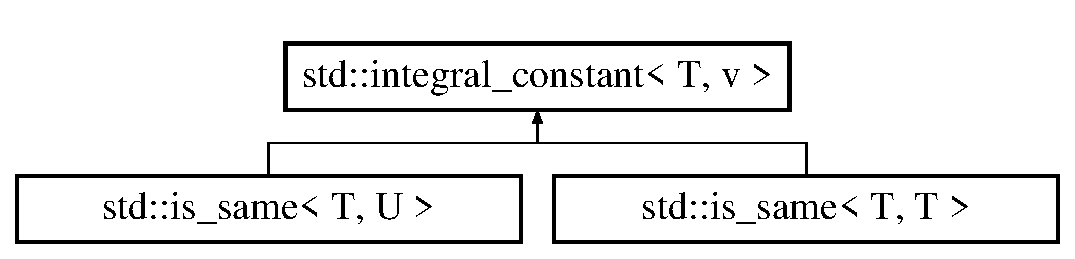
\includegraphics[height=2.000000cm]{da/dcf/structstd_1_1integral__constant}
\end{center}
\end{figure}
\subsection*{Public Types}
\begin{DoxyCompactItemize}
\item 
\hypertarget{structstd_1_1integral__constant_a577f947f94f81e5992b37a1748a51d97}{}\label{structstd_1_1integral__constant_a577f947f94f81e5992b37a1748a51d97} 
typedef T {\bfseries value\+\_\+type}
\item 
\hypertarget{structstd_1_1integral__constant_ab0ee496d528433edf4b782e6fcd47d1e}{}\label{structstd_1_1integral__constant_ab0ee496d528433edf4b782e6fcd47d1e} 
typedef \hyperlink{structstd_1_1integral__constant}{integral\+\_\+constant} {\bfseries type}
\end{DoxyCompactItemize}
\subsection*{Public Member Functions}
\begin{DoxyCompactItemize}
\item 
\hypertarget{structstd_1_1integral__constant_a63cf3115ee14c1bf3e87730d41b3fea3}{}\label{structstd_1_1integral__constant_a63cf3115ee14c1bf3e87730d41b3fea3} 
constexpr {\bfseries operator value\+\_\+type} () const noexcept
\item 
\hypertarget{structstd_1_1integral__constant_a3dc39a4cfefa5334de46c5d2f93b9910}{}\label{structstd_1_1integral__constant_a3dc39a4cfefa5334de46c5d2f93b9910} 
constexpr value\+\_\+type {\bfseries operator()} () const noexcept
\end{DoxyCompactItemize}
\subsection*{Static Public Attributes}
\begin{DoxyCompactItemize}
\item 
\hypertarget{structstd_1_1integral__constant_aeb13450790039d71c68069a97a9fad40}{}\label{structstd_1_1integral__constant_aeb13450790039d71c68069a97a9fad40} 
static constexpr T {\bfseries value} = v
\end{DoxyCompactItemize}


The documentation for this struct was generated from the following file\+:\begin{DoxyCompactItemize}
\item 
src/type\+\_\+traits.\+h\end{DoxyCompactItemize}

\hypertarget{structstd_1_1is__same}{}\section{std\+:\+:is\+\_\+same$<$ T, U $>$ Struct Template Reference}
\label{structstd_1_1is__same}\index{std\+::is\+\_\+same$<$ T, U $>$@{std\+::is\+\_\+same$<$ T, U $>$}}
Inheritance diagram for std\+:\+:is\+\_\+same$<$ T, U $>$\+:\begin{figure}[H]
\begin{center}
\leavevmode
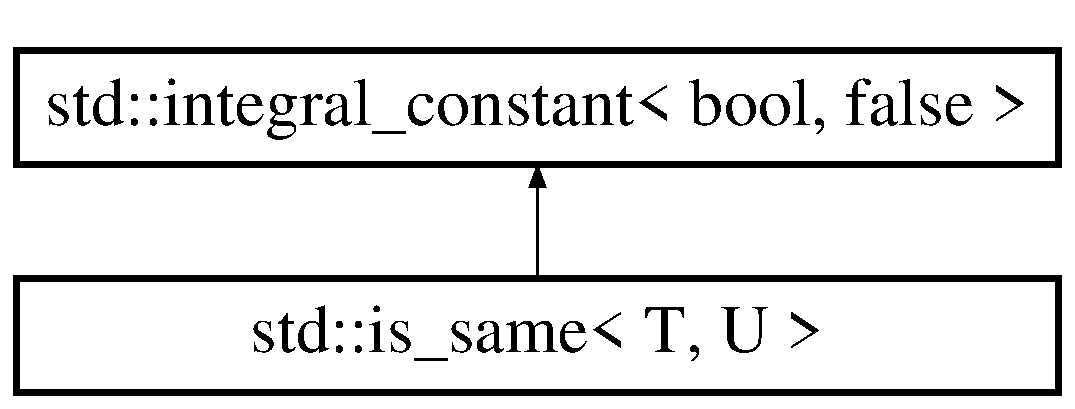
\includegraphics[height=2.000000cm]{d8/d4f/structstd_1_1is__same}
\end{center}
\end{figure}
\subsection*{Additional Inherited Members}


The documentation for this struct was generated from the following file\+:\begin{DoxyCompactItemize}
\item 
src/type\+\_\+traits.\+h\end{DoxyCompactItemize}

\hypertarget{structstd_1_1is__same_3_01T_00_01T_01_4}{}\section{std\+:\+:is\+\_\+same$<$ T, T $>$ Struct Template Reference}
\label{structstd_1_1is__same_3_01T_00_01T_01_4}\index{std\+::is\+\_\+same$<$ T, T $>$@{std\+::is\+\_\+same$<$ T, T $>$}}
Inheritance diagram for std\+:\+:is\+\_\+same$<$ T, T $>$\+:\begin{figure}[H]
\begin{center}
\leavevmode
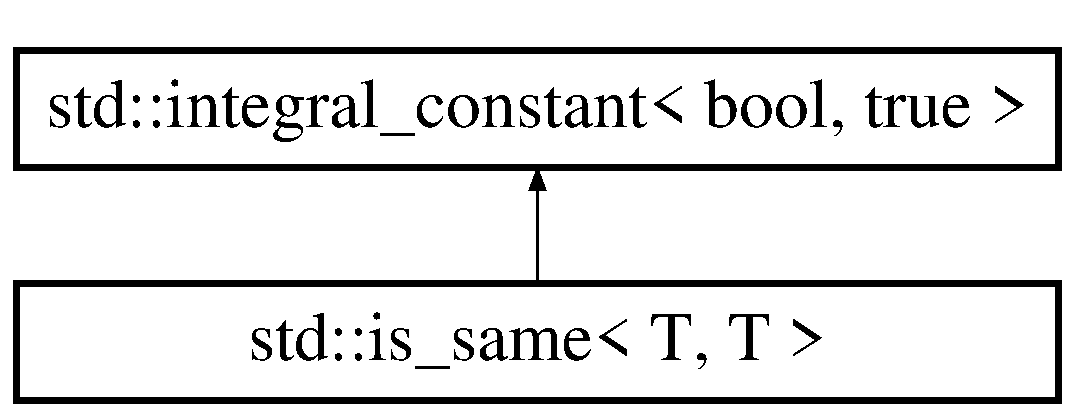
\includegraphics[height=2.000000cm]{d1/db4/structstd_1_1is__same_3_01T_00_01T_01_4}
\end{center}
\end{figure}
\subsection*{Additional Inherited Members}


The documentation for this struct was generated from the following file\+:\begin{DoxyCompactItemize}
\item 
src/type\+\_\+traits.\+h\end{DoxyCompactItemize}

\hypertarget{classLcd}{}\section{Lcd$<$ L\+C\+D\+\_\+\+D7, L\+C\+D\+\_\+\+D6, L\+C\+D\+\_\+\+D5, L\+C\+D\+\_\+\+D4, L\+C\+D\+\_\+\+E\+N\+A\+B\+LE, L\+C\+D\+\_\+\+R\+E\+G\+\_\+\+S\+E\+L\+E\+CT $>$ Class Template Reference}
\label{classLcd}\index{Lcd$<$ L\+C\+D\+\_\+\+D7, L\+C\+D\+\_\+\+D6, L\+C\+D\+\_\+\+D5, L\+C\+D\+\_\+\+D4, L\+C\+D\+\_\+\+E\+N\+A\+B\+L\+E, L\+C\+D\+\_\+\+R\+E\+G\+\_\+\+S\+E\+L\+E\+C\+T $>$@{Lcd$<$ L\+C\+D\+\_\+\+D7, L\+C\+D\+\_\+\+D6, L\+C\+D\+\_\+\+D5, L\+C\+D\+\_\+\+D4, L\+C\+D\+\_\+\+E\+N\+A\+B\+L\+E, L\+C\+D\+\_\+\+R\+E\+G\+\_\+\+S\+E\+L\+E\+C\+T $>$}}
\subsection*{Public Types}
\begin{DoxyCompactItemize}
\item 
typedef \hyperlink{classLcd}{Lcd}$<$ L\+C\+D\+\_\+\+D7, L\+C\+D\+\_\+\+D6, L\+C\+D\+\_\+\+D5, L\+C\+D\+\_\+\+D4, L\+C\+D\+\_\+\+E\+N\+A\+B\+LE, L\+C\+D\+\_\+\+R\+E\+G\+\_\+\+S\+E\+L\+E\+CT $>$ {\bfseries \+\_\+\+Lcd}\hypertarget{classLcd_ae69976feb51799d3e9991dd74b060675}{}\label{classLcd_ae69976feb51799d3e9991dd74b060675}

\end{DoxyCompactItemize}
\subsection*{Public Member Functions}
\begin{DoxyCompactItemize}
\item 
{\footnotesize template$<$typename T $>$ }\\\hyperlink{classLcd}{\+\_\+\+Lcd} \& {\bfseries operator$<$$<$} (const T \&t)\hypertarget{classLcd_ae12b6a315191a6be957d0da7479f8e7c}{}\label{classLcd_ae12b6a315191a6be957d0da7479f8e7c}

\end{DoxyCompactItemize}
\subsection*{Static Public Member Functions}
\begin{DoxyCompactItemize}
\item 
static void {\bfseries io\+\_\+init} ()\hypertarget{classLcd_a74bcd553e61d9f9c052a2ada7696c1e6}{}\label{classLcd_a74bcd553e61d9f9c052a2ada7696c1e6}

\item 
static void {\bfseries command} (const uint8\+\_\+t \&command)\hypertarget{classLcd_ac7183eb4a448aa052c49503c902ca261}{}\label{classLcd_ac7183eb4a448aa052c49503c902ca261}

\item 
static void {\bfseries data} (const uint8\+\_\+t \&data)\hypertarget{classLcd_a12e1dfd8741ff8f9abcf4cedb976f46e}{}\label{classLcd_a12e1dfd8741ff8f9abcf4cedb976f46e}

\item 
static void {\bfseries init} ()\hypertarget{classLcd_aefedfd3decc17d6c0a250a15af9053ac}{}\label{classLcd_aefedfd3decc17d6c0a250a15af9053ac}

\item 
{\footnotesize template$<$typename T $>$ }\\static void {\bfseries print} (const T \&t)\hypertarget{classLcd_ad6128575affb14846b529c8453a1a5a8}{}\label{classLcd_ad6128575affb14846b529c8453a1a5a8}

\item 
static void {\bfseries set\+\_\+display\+\_\+address} (const uint8\+\_\+t \&pos)\hypertarget{classLcd_a45f400406b7cb57ee26d5eab703b6d1a}{}\label{classLcd_a45f400406b7cb57ee26d5eab703b6d1a}

\end{DoxyCompactItemize}


The documentation for this class was generated from the following file\+:\begin{DoxyCompactItemize}
\item 
src/lcd.\+h\end{DoxyCompactItemize}

\hypertarget{classMatrixButtons}{}\section{Matrix\+Buttons$<$ Row\+List, Column\+List, Listener $>$ Class Template Reference}
\label{classMatrixButtons}\index{Matrix\+Buttons$<$ Row\+List, Column\+List, Listener $>$@{Matrix\+Buttons$<$ Row\+List, Column\+List, Listener $>$}}
\subsection*{Static Public Member Functions}
\begin{DoxyCompactItemize}
\item 
\hypertarget{classMatrixButtons_a28aaefa849e34b188d2a74293ead0e41}{}\label{classMatrixButtons_a28aaefa849e34b188d2a74293ead0e41} 
static void {\bfseries init} ()
\item 
\hypertarget{classMatrixButtons_a8a751df6ba30a66be953d4098e8eadb3}{}\label{classMatrixButtons_a8a751df6ba30a66be953d4098e8eadb3} 
{\footnotesize template$<$typename T $>$ }\\static T {\bfseries run} (const T \&clock)
\item 
\hypertarget{classMatrixButtons_ac9394408a6020172ef35dfaebed40784}{}\label{classMatrixButtons_ac9394408a6020172ef35dfaebed40784} 
static uint8\+\_\+t {\bfseries is\+\_\+enabled} ()
\end{DoxyCompactItemize}


The documentation for this class was generated from the following file\+:\begin{DoxyCompactItemize}
\item 
src/buttons.\+h\end{DoxyCompactItemize}

\hypertarget{classModbus}{}\section{Modbus$<$ address\+Id, Modbus\+Data\+List, Connection\+Ctrl $>$ Class Template Reference}
\label{classModbus}\index{Modbus$<$ address\+Id, Modbus\+Data\+List, Connection\+Ctrl $>$@{Modbus$<$ address\+Id, Modbus\+Data\+List, Connection\+Ctrl $>$}}
\subsection*{Static Public Member Functions}
\begin{DoxyCompactItemize}
\item 
static void {\bfseries reset} ()\hypertarget{classModbus_af1b825d738f689a73996322cb97a3731}{}\label{classModbus_af1b825d738f689a73996322cb97a3731}

\item 
static uint8\+\_\+t {\bfseries can\+\_\+rx} ()\hypertarget{classModbus_aa01e2f99ffceaf529d50a046c181cb6f}{}\label{classModbus_aa01e2f99ffceaf529d50a046c181cb6f}

\item 
static void {\bfseries rx} (uint8\+\_\+t c)\hypertarget{classModbus_af8c1c0ad33aae3f95654dde48e899dbe}{}\label{classModbus_af8c1c0ad33aae3f95654dde48e899dbe}

\item 
static uint8\+\_\+t {\bfseries tx\+\_\+is\+\_\+empty} ()\hypertarget{classModbus_a0a043d814f91d12d22abeb756ec56391}{}\label{classModbus_a0a043d814f91d12d22abeb756ec56391}

\item 
static uint8\+\_\+t {\bfseries tx\+\_\+pop} ()\hypertarget{classModbus_a13acf7f89171aeda9822d47d53cf178b}{}\label{classModbus_a13acf7f89171aeda9822d47d53cf178b}

\item 
static void {\bfseries process} ()\hypertarget{classModbus_a71101c24dca8e920e83baf536433c4c1}{}\label{classModbus_a71101c24dca8e920e83baf536433c4c1}

\item 
static uint8\+\_\+t {\bfseries is\+\_\+enabled} ()\hypertarget{classModbus_af486735a2aa3a896e02753bd58c6dd9a}{}\label{classModbus_af486735a2aa3a896e02753bd58c6dd9a}

\item 
{\footnotesize template$<$typename T $>$ }\\static T {\bfseries run} (const T \&clock)\hypertarget{classModbus_a2d1a0d2149fd976590667356aa983343}{}\label{classModbus_a2d1a0d2149fd976590667356aa983343}

\end{DoxyCompactItemize}


The documentation for this class was generated from the following file\+:\begin{DoxyCompactItemize}
\item 
src/modbus.\+h\end{DoxyCompactItemize}

\hypertarget{struct__timer0_1_1ModeSupport}{}\section{\+\_\+timer0\+:\+:Mode\+Support$<$ Mode, Clock\+Select $>$ Struct Template Reference}
\label{struct__timer0_1_1ModeSupport}\index{\+\_\+timer0\+::\+Mode\+Support$<$ Mode, Clock\+Select $>$@{\+\_\+timer0\+::\+Mode\+Support$<$ Mode, Clock\+Select $>$}}


The documentation for this struct was generated from the following file\+:\begin{DoxyCompactItemize}
\item 
src/timer0.\+h\end{DoxyCompactItemize}

\hypertarget{class__spi_1_1NoSS}{}\section{\+\_\+spi\+:\+:No\+SS Class Reference}
\label{class__spi_1_1NoSS}\index{\+\_\+spi\+::\+No\+SS@{\+\_\+spi\+::\+No\+SS}}


The documentation for this class was generated from the following file\+:\begin{DoxyCompactItemize}
\item 
src/spi.\+h\end{DoxyCompactItemize}

\hypertarget{classstd_1_1numeric__limits}{}\section{std\+:\+:numeric\+\_\+limits$<$ T $>$ Class Template Reference}
\label{classstd_1_1numeric__limits}\index{std\+::numeric\+\_\+limits$<$ T $>$@{std\+::numeric\+\_\+limits$<$ T $>$}}
\subsection*{Static Public Member Functions}
\begin{DoxyCompactItemize}
\item 
static uint8\+\_\+t {\bfseries is\+\_\+signed} ()\hypertarget{classstd_1_1numeric__limits_a0c0397b435b08d7f7b629dc264ad6b39}{}\label{classstd_1_1numeric__limits_a0c0397b435b08d7f7b629dc264ad6b39}

\item 
static uint8\+\_\+t {\bfseries digits} ()\hypertarget{classstd_1_1numeric__limits_aa7a4f181eb6e5b26661ed2c6c6ab653b}{}\label{classstd_1_1numeric__limits_aa7a4f181eb6e5b26661ed2c6c6ab653b}

\item 
static T {\bfseries max} ()\hypertarget{classstd_1_1numeric__limits_ae5fc707d9d6ebbac808a5fb6e26690f8}{}\label{classstd_1_1numeric__limits_ae5fc707d9d6ebbac808a5fb6e26690f8}

\end{DoxyCompactItemize}


The documentation for this class was generated from the following file\+:\begin{DoxyCompactItemize}
\item 
src/limits.\+h\end{DoxyCompactItemize}

\hypertarget{classstd_1_1numeric__limits_3_01uint16__t_01_4}{}\section{std\+:\+:numeric\+\_\+limits$<$ uint16\+\_\+t $>$ Class Template Reference}
\label{classstd_1_1numeric__limits_3_01uint16__t_01_4}\index{std\+::numeric\+\_\+limits$<$ uint16\+\_\+t $>$@{std\+::numeric\+\_\+limits$<$ uint16\+\_\+t $>$}}
\subsection*{Static Public Member Functions}
\begin{DoxyCompactItemize}
\item 
\hypertarget{classstd_1_1numeric__limits_3_01uint16__t_01_4_afb86f68ec1ed3973f6112457d8fa25bb}{}\label{classstd_1_1numeric__limits_3_01uint16__t_01_4_afb86f68ec1ed3973f6112457d8fa25bb} 
static uint8\+\_\+t {\bfseries is\+\_\+signed} ()
\item 
\hypertarget{classstd_1_1numeric__limits_3_01uint16__t_01_4_af8baf757e5505a7ee8c78f1e5f98f285}{}\label{classstd_1_1numeric__limits_3_01uint16__t_01_4_af8baf757e5505a7ee8c78f1e5f98f285} 
static uint8\+\_\+t {\bfseries digits} ()
\item 
\hypertarget{classstd_1_1numeric__limits_3_01uint16__t_01_4_ac51d5d78ead4199574e0831c136ca395}{}\label{classstd_1_1numeric__limits_3_01uint16__t_01_4_ac51d5d78ead4199574e0831c136ca395} 
static uint16\+\_\+t {\bfseries max} ()
\end{DoxyCompactItemize}


The documentation for this class was generated from the following file\+:\begin{DoxyCompactItemize}
\item 
src/limits.\+h\end{DoxyCompactItemize}

\hypertarget{classstd_1_1numeric__limits_3_01uint8__t_01_4}{}\section{std\+:\+:numeric\+\_\+limits$<$ uint8\+\_\+t $>$ Class Template Reference}
\label{classstd_1_1numeric__limits_3_01uint8__t_01_4}\index{std\+::numeric\+\_\+limits$<$ uint8\+\_\+t $>$@{std\+::numeric\+\_\+limits$<$ uint8\+\_\+t $>$}}
\subsection*{Static Public Member Functions}
\begin{DoxyCompactItemize}
\item 
\hypertarget{classstd_1_1numeric__limits_3_01uint8__t_01_4_adcbd633b68edddbf4197919ab60bb9fd}{}\label{classstd_1_1numeric__limits_3_01uint8__t_01_4_adcbd633b68edddbf4197919ab60bb9fd} 
static uint8\+\_\+t {\bfseries is\+\_\+signed} ()
\item 
\hypertarget{classstd_1_1numeric__limits_3_01uint8__t_01_4_a60652abaf60fe4ad2b9634e0281d9468}{}\label{classstd_1_1numeric__limits_3_01uint8__t_01_4_a60652abaf60fe4ad2b9634e0281d9468} 
static uint8\+\_\+t {\bfseries digits} ()
\item 
\hypertarget{classstd_1_1numeric__limits_3_01uint8__t_01_4_a08e857684300f5f5d5e973e40af90a5d}{}\label{classstd_1_1numeric__limits_3_01uint8__t_01_4_a08e857684300f5f5d5e973e40af90a5d} 
static uint8\+\_\+t {\bfseries max} ()
\end{DoxyCompactItemize}


The documentation for this class was generated from the following file\+:\begin{DoxyCompactItemize}
\item 
src/limits.\+h\end{DoxyCompactItemize}

\hypertarget{classPgmDataPtr}{}\section{Pgm\+Data\+Ptr$<$ T $>$ Class Template Reference}
\label{classPgmDataPtr}\index{Pgm\+Data\+Ptr$<$ T $>$@{Pgm\+Data\+Ptr$<$ T $>$}}
\subsection*{Public Types}
\begin{DoxyCompactItemize}
\item 
\hypertarget{classPgmDataPtr_a1c723887632424e9f6fb422cf3725d5b}{}\label{classPgmDataPtr_a1c723887632424e9f6fb422cf3725d5b} 
typedef const T $\ast$ {\bfseries type\+\_\+t}
\end{DoxyCompactItemize}
\subsection*{Public Member Functions}
\begin{DoxyCompactItemize}
\item 
\hypertarget{classPgmDataPtr_a81d95a9f569ab29401a005395df50257}{}\label{classPgmDataPtr_a81d95a9f569ab29401a005395df50257} 
type\+\_\+t {\bfseries get} () const
\end{DoxyCompactItemize}
\subsection*{Static Public Member Functions}
\begin{DoxyCompactItemize}
\item 
\hypertarget{classPgmDataPtr_a4ca4a1c1032d8f8092fc2b46426e2566}{}\label{classPgmDataPtr_a4ca4a1c1032d8f8092fc2b46426e2566} 
{\footnotesize template$<$typename V $>$ }\\static const \hyperlink{classPgmDataPtr}{Pgm\+Data\+Ptr}$<$ V $>$ $\ast$ {\bfseries ptr} (const V $\ast$v)
\end{DoxyCompactItemize}


The documentation for this class was generated from the following file\+:\begin{DoxyCompactItemize}
\item 
src/pgmspace.\+h\end{DoxyCompactItemize}

\hypertarget{structports_1_1Pin}{}\section{ports\+:\+:Pin$<$ p, b $>$ Struct Template Reference}
\label{structports_1_1Pin}\index{ports\+::\+Pin$<$ p, b $>$@{ports\+::\+Pin$<$ p, b $>$}}


Every pin has one ore multiple typedefs of this class.  




{\ttfamily \#include $<$ports.\+h$>$}

\subsection*{Public Types}
\begin{DoxyCompactItemize}
\item 
typedef \hyperlink{structports_1_1__Io}{\+\_\+\+Io}$<$ p, b, \+\_\+\+I\+O\+Reg\+::\+D\+D\+Rx $>$ {\bfseries \+\_\+\+D\+DR}\hypertarget{structports_1_1Pin_a520a470d63ee662a6e32050e23118405}{}\label{structports_1_1Pin_a520a470d63ee662a6e32050e23118405}

\item 
typedef \hyperlink{structports_1_1__Io}{\+\_\+\+Io}$<$ p, b, \+\_\+\+I\+O\+Reg\+::\+P\+O\+R\+Tx $>$ {\bfseries \+\_\+\+P\+O\+RT}\hypertarget{structports_1_1Pin_a21300f49ada5e9c43c8c7fd3c5d02bab}{}\label{structports_1_1Pin_a21300f49ada5e9c43c8c7fd3c5d02bab}

\item 
typedef \hyperlink{structports_1_1__Io}{\+\_\+\+Io}$<$ p, b, \+\_\+\+I\+O\+Reg\+::\+P\+I\+Nx $>$ {\bfseries \+\_\+\+P\+IN}\hypertarget{structports_1_1Pin_a11990dc8597439185ba300ee0bbc54e6}{}\label{structports_1_1Pin_a11990dc8597439185ba300ee0bbc54e6}

\end{DoxyCompactItemize}
\subsection*{Static Public Member Functions}
\begin{DoxyCompactItemize}
\item 
static void \hyperlink{structports_1_1Pin_a0ab0631ab14e62fd6f131005e96c298c}{set\+DD} (const enum \hyperlink{namespaceports_a46987e78fa447129742fadda5eccafb4}{Data\+Direction} dd)\hypertarget{structports_1_1Pin_a0ab0631ab14e62fd6f131005e96c298c}{}\label{structports_1_1Pin_a0ab0631ab14e62fd6f131005e96c298c}

\begin{DoxyCompactList}\small\item\em Equivalent to {\ttfamily D\+DR = dd;}. \end{DoxyCompactList}\item 
static enum \hyperlink{namespaceports_a46987e78fa447129742fadda5eccafb4}{Data\+Direction} \hyperlink{structports_1_1Pin_a7aabcc753e62bd94ee9a8186e9d050ab}{get\+DD} ()\hypertarget{structports_1_1Pin_a7aabcc753e62bd94ee9a8186e9d050ab}{}\label{structports_1_1Pin_a7aabcc753e62bd94ee9a8186e9d050ab}

\begin{DoxyCompactList}\small\item\em returns either Data\+Direction\+::\+In or Data\+Direction\+::\+Output by reading from D\+DR and casting the bit value. \end{DoxyCompactList}\item 
static void \hyperlink{structports_1_1Pin_a11ba9e7aeda2d867780dee32234f2c7e}{set\+Pull\+Up} (const enum \hyperlink{namespaceports_a49bf0ccedb4cfed89a328574e53bec07}{Pull\+Up} pull\+Up)\hypertarget{structports_1_1Pin_a11ba9e7aeda2d867780dee32234f2c7e}{}\label{structports_1_1Pin_a11ba9e7aeda2d867780dee32234f2c7e}

\begin{DoxyCompactList}\small\item\em Equivalent to {\ttfamily P\+O\+RT = pull\+Up;}. \end{DoxyCompactList}\item 
static enum \hyperlink{namespaceports_a49bf0ccedb4cfed89a328574e53bec07}{Pull\+Up} \hyperlink{structports_1_1Pin_a5a5e3c8e256954043d749752859ea300}{get\+Pull\+Up} ()\hypertarget{structports_1_1Pin_a5a5e3c8e256954043d749752859ea300}{}\label{structports_1_1Pin_a5a5e3c8e256954043d749752859ea300}

\begin{DoxyCompactList}\small\item\em returns either Pull\+Up\+::\+Off or Pull\+Up\+::\+On by reading from P\+O\+RT and casting the bit value. \end{DoxyCompactList}\item 
static void \hyperlink{structports_1_1Pin_ae2f380ea5586a2eaa6e0d0b85dbf0983}{set\+To\+Input} (const enum \hyperlink{namespaceports_a49bf0ccedb4cfed89a328574e53bec07}{Pull\+Up} pull\+Up)\hypertarget{structports_1_1Pin_ae2f380ea5586a2eaa6e0d0b85dbf0983}{}\label{structports_1_1Pin_ae2f380ea5586a2eaa6e0d0b85dbf0983}

\begin{DoxyCompactList}\small\item\em Equivalent to first setting the data direction {\ttfamily D\+DR = Data\+Direction\+::\+Input;} followed by setting the pull up resistor\+: {\ttfamily P\+O\+RT = pullup;}. \end{DoxyCompactList}\item 
static void \hyperlink{structports_1_1Pin_a3caf6009548ed46020910f36d2b0f4f9}{toggle} ()\hypertarget{structports_1_1Pin_a3caf6009548ed46020910f36d2b0f4f9}{}\label{structports_1_1Pin_a3caf6009548ed46020910f36d2b0f4f9}

\begin{DoxyCompactList}\small\item\em Equivalent to {\ttfamily P\+IN = 1;} which toggles the output if pin is in output mode. \end{DoxyCompactList}\end{DoxyCompactItemize}
\subsection*{Static Public Attributes}
\begin{DoxyCompactItemize}
\item 
static enum \hyperlink{namespaceports_a9949317f344930bd6ad1097e80c97b67}{\+\_\+\+Port} \hyperlink{structports_1_1Pin_ad63613b8c14441d28e3f3d935da67e77}{port} = p\hypertarget{structports_1_1Pin_ad63613b8c14441d28e3f3d935da67e77}{}\label{structports_1_1Pin_ad63613b8c14441d28e3f3d935da67e77}

\begin{DoxyCompactList}\small\item\em The port name (enum \+\_\+\+Port) of this pin. \end{DoxyCompactList}\item 
static const uint8\+\_\+t \hyperlink{structports_1_1Pin_aea726b85cfe5e49822dd2517da5c860f}{bit} = b\hypertarget{structports_1_1Pin_aea726b85cfe5e49822dd2517da5c860f}{}\label{structports_1_1Pin_aea726b85cfe5e49822dd2517da5c860f}

\begin{DoxyCompactList}\small\item\em The bit position (0-\/7) inside the D\+D\+Rx, P\+O\+R\+Tx or P\+I\+Nx register. \end{DoxyCompactList}\item 
static \hyperlink{structports_1_1__Io}{\+\_\+\+D\+DR} \hyperlink{structports_1_1Pin_aaebb4d6cb5db0635fe8e7d6e7d315c7f}{D\+DR}
\begin{DoxyCompactList}\small\item\em Simplified access to the D\+DR value of this pin. \end{DoxyCompactList}\item 
static \hyperlink{structports_1_1__Io}{\+\_\+\+P\+O\+RT} \hyperlink{structports_1_1Pin_aaa08f0eb17ef31d9f46d65d50c8a093e}{P\+O\+RT}
\begin{DoxyCompactList}\small\item\em Simplified access to the P\+O\+RT value of this pin. \end{DoxyCompactList}\item 
static \hyperlink{structports_1_1__Io}{\+\_\+\+P\+IN} \hyperlink{structports_1_1Pin_ae2e45a41082457c350f71f7a720265d4}{P\+IN}
\begin{DoxyCompactList}\small\item\em Simplified access to the P\+IN value of this pin. \end{DoxyCompactList}\end{DoxyCompactItemize}


\subsection{Detailed Description}
\subsubsection*{template$<$enum \+\_\+\+Port p, uint8\+\_\+t b$>$\\*
struct ports\+::\+Pin$<$ p, b $>$}

Every pin has one ore multiple typedefs of this class. 

The port name (enum \+\_\+\+Port) and the bit in the registers is provided as static variables.

In addition reading or setting the value of a pin is simplified through \hyperlink{structports_1_1Pin_aaebb4d6cb5db0635fe8e7d6e7d315c7f}{D\+DR} \hyperlink{structports_1_1Pin_aaa08f0eb17ef31d9f46d65d50c8a093e}{P\+O\+RT} and \hyperlink{structports_1_1Pin_ae2e45a41082457c350f71f7a720265d4}{P\+IN} which have cast converters from uint8\+\_\+t.

Using those static members (\hyperlink{structports_1_1Pin_aaebb4d6cb5db0635fe8e7d6e7d315c7f}{D\+DR}, \hyperlink{structports_1_1Pin_aaa08f0eb17ef31d9f46d65d50c8a093e}{P\+O\+RT} or \hyperlink{structports_1_1Pin_ae2e45a41082457c350f71f7a720265d4}{P\+IN}) liberates you from writing bit operations. If your pin is for instance B2, a typical way to set the D\+DR value of the pin to 0 would have been\+: {\ttfamily P\+O\+R\+TB \&= $\sim$(\+\_\+\+B\+V(2));}

The exact same thing may now be done by writing\+: {\ttfamily \hyperlink{structports_1_1Pin_aaebb4d6cb5db0635fe8e7d6e7d315c7f}{P\+I\+N\+\_\+\+B2\+::\+D\+DR} = 0;}

When using the enums \hyperlink{namespaceports_a46987e78fa447129742fadda5eccafb4}{Data\+Direction} or \hyperlink{namespaceports_a49bf0ccedb4cfed89a328574e53bec07}{Pull\+Up} the compiler verifies that the enum is used for the correct register.

The compiler does not verify that you are in the correct \char`\"{}mode\char`\"{}. Calling \hyperlink{structports_1_1Pin_a11ba9e7aeda2d867780dee32234f2c7e}{set\+Pull\+Up()} when the pin is in output mode will change the output! You would need to switch to input first ({\ttfamily D\+DR = Data\+Direction\+::\+Input;}). 

\subsection{Member Data Documentation}
\index{ports\+::\+Pin@{ports\+::\+Pin}!D\+DR@{D\+DR}}
\index{D\+DR@{D\+DR}!ports\+::\+Pin@{ports\+::\+Pin}}
\subsubsection[{\texorpdfstring{D\+DR}{DDR}}]{\setlength{\rightskip}{0pt plus 5cm}template$<$enum \+\_\+\+Port p, uint8\+\_\+t b$>$ {\bf Pin}$<$ p, b $>$\+::{\bf \+\_\+\+D\+DR} {\bf ports\+::\+Pin}$<$ p, b $>$\+::D\+DR\hspace{0.3cm}{\ttfamily [static]}}\hypertarget{structports_1_1Pin_aaebb4d6cb5db0635fe8e7d6e7d315c7f}{}\label{structports_1_1Pin_aaebb4d6cb5db0635fe8e7d6e7d315c7f}


Simplified access to the D\+DR value of this pin. 

A cast operator of this variable allows you to read and write the D\+DR value for this bit as if every bit had its own {\ttfamily uint8\+\_\+t}.

Cast operators to and from enum \hyperlink{namespaceports_a46987e78fa447129742fadda5eccafb4}{Data\+Direction} are also implemented and prevent accidental use of an incorrect register.

Examples\+:


\begin{DoxyItemize}
\item {\ttfamily P\+O\+R\+T\+\_\+\+C3\+::\+D\+DR = Data\+Direction\+::\+Input;}
\item {\ttfamily uint8\+\_\+t current\+D\+DR = P\+O\+R\+T\+\_\+\+C3\+::\+D\+DR;}
\item {\ttfamily enum Data\+Direction current\+D\+D\+R2 = P\+O\+R\+T\+\_\+\+C3\+::\+D\+DR;} 
\end{DoxyItemize}\index{ports\+::\+Pin@{ports\+::\+Pin}!P\+IN@{P\+IN}}
\index{P\+IN@{P\+IN}!ports\+::\+Pin@{ports\+::\+Pin}}
\subsubsection[{\texorpdfstring{P\+IN}{PIN}}]{\setlength{\rightskip}{0pt plus 5cm}template$<$enum \+\_\+\+Port p, uint8\+\_\+t b$>$ {\bf Pin}$<$ p, b $>$\+::{\bf \+\_\+\+P\+IN} {\bf ports\+::\+Pin}$<$ p, b $>$\+::P\+IN\hspace{0.3cm}{\ttfamily [static]}}\hypertarget{structports_1_1Pin_ae2e45a41082457c350f71f7a720265d4}{}\label{structports_1_1Pin_ae2e45a41082457c350f71f7a720265d4}


Simplified access to the P\+IN value of this pin. 

A cast operator of this variable allows you to read and write the D\+DR value for this bit as if every bit had its own uint8\+\_\+t.

Examples\+:


\begin{DoxyItemize}
\item {\ttfamily P\+O\+R\+T\+\_\+\+C3\+::\+D\+DR = Data\+Direction\+::\+Input;}
\item {\ttfamily uint8\+\_\+t current\+D\+DR = P\+O\+R\+T\+\_\+\+C3\+::\+D\+DR;}
\item {\ttfamily Data\+Direction current\+D\+D\+R2 = P\+O\+R\+T\+\_\+\+C3\+::\+D\+DR;} 
\end{DoxyItemize}\index{ports\+::\+Pin@{ports\+::\+Pin}!P\+O\+RT@{P\+O\+RT}}
\index{P\+O\+RT@{P\+O\+RT}!ports\+::\+Pin@{ports\+::\+Pin}}
\subsubsection[{\texorpdfstring{P\+O\+RT}{PORT}}]{\setlength{\rightskip}{0pt plus 5cm}template$<$enum \+\_\+\+Port p, uint8\+\_\+t b$>$ {\bf Pin}$<$ p, b $>$\+::{\bf \+\_\+\+P\+O\+RT} {\bf ports\+::\+Pin}$<$ p, b $>$\+::P\+O\+RT\hspace{0.3cm}{\ttfamily [static]}}\hypertarget{structports_1_1Pin_aaa08f0eb17ef31d9f46d65d50c8a093e}{}\label{structports_1_1Pin_aaa08f0eb17ef31d9f46d65d50c8a093e}


Simplified access to the P\+O\+RT value of this pin. 

A cast operator of this variable allows you to read and write the P\+O\+RT value for this bit as if every bit had its own {\ttfamily uint8\+\_\+t}.

Cast operators to and from enum \hyperlink{namespaceports_a49bf0ccedb4cfed89a328574e53bec07}{Pull\+Up} are also implemented and prevent accidental use of an incorrect register.

Examples\+:


\begin{DoxyItemize}
\item {\ttfamily P\+O\+R\+T\+\_\+\+A\+D\+C4\+::\+P\+O\+RT = 1;}
\item {\ttfamily uint8\+\_\+t current\+Port = P\+O\+R\+T\+\_\+\+A\+D\+C4\+::\+P\+O\+RT;}
\item {\ttfamily enum Pull\+Up current\+Pull\+Up = P\+O\+R\+T\+\_\+\+A\+D\+C4\+::\+P\+O\+RT;} 
\end{DoxyItemize}

The documentation for this struct was generated from the following file\+:\begin{DoxyCompactItemize}
\item 
src/ports.\+h\end{DoxyCompactItemize}

\hypertarget{class__buttons_1_1PinList}{}\section{\+\_\+buttons\+:\+:Pin\+List$<$ Pins $>$ Class Template Reference}
\label{class__buttons_1_1PinList}\index{\+\_\+buttons\+::\+Pin\+List$<$ Pins $>$@{\+\_\+buttons\+::\+Pin\+List$<$ Pins $>$}}


The documentation for this class was generated from the following file\+:\begin{DoxyCompactItemize}
\item 
src/buttons.\+h\end{DoxyCompactItemize}

\hypertarget{classPulseUartTx}{}\section{Pulse\+Uart\+Tx$<$ Tx\+Pin, zero\+Bit\+Duration, \+\_\+tx\+\_\+buffer\+\_\+size, Task, one\+Bit\+Duration, sync\+Bit\+Duration, inverse\+Output $>$ Class Template Reference}
\label{classPulseUartTx}\index{Pulse\+Uart\+Tx$<$ Tx\+Pin, zero\+Bit\+Duration, \+\_\+tx\+\_\+buffer\+\_\+size, Task, one\+Bit\+Duration, sync\+Bit\+Duration, inverse\+Output $>$@{Pulse\+Uart\+Tx$<$ Tx\+Pin, zero\+Bit\+Duration, \+\_\+tx\+\_\+buffer\+\_\+size, Task, one\+Bit\+Duration, sync\+Bit\+Duration, inverse\+Output $>$}}
\subsection*{Public Member Functions}
\begin{DoxyCompactItemize}
\item 
\hypertarget{classPulseUartTx_a591f65d2a373b53cef046a0caa09f86a}{}\label{classPulseUartTx_a591f65d2a373b53cef046a0caa09f86a} 
{\footnotesize template$<$typename T $>$ }\\\hyperlink{classPulseUartTx}{\+\_\+\+Pulse\+Uart\+Tx} \& {\bfseries operator$<$$<$} (const T \&t)
\end{DoxyCompactItemize}
\subsection*{Static Public Member Functions}
\begin{DoxyCompactItemize}
\item 
\hypertarget{classPulseUartTx_afe1716e309086b7419aaca036f0e0c16}{}\label{classPulseUartTx_afe1716e309086b7419aaca036f0e0c16} 
static void {\bfseries init} ()
\item 
\hypertarget{classPulseUartTx_a5a80e32bf9c301830f710d5b8d379259}{}\label{classPulseUartTx_a5a80e32bf9c301830f710d5b8d379259} 
{\footnotesize template$<$typename T $>$ }\\static void {\bfseries tx} (const T \&t)
\end{DoxyCompactItemize}


The documentation for this class was generated from the following file\+:\begin{DoxyCompactItemize}
\item 
src/pulse\+\_\+uart.\+h\end{DoxyCompactItemize}

\hypertarget{classPwm}{}\section{Pwm$<$ TimerN, Mode, Out\+ModeA, Out\+ModeB, Set\+D\+D\+R\+\_\+A, Set\+D\+D\+R\+\_\+B, TaskA, TaskB, Task\+OvF $>$ Class Template Reference}
\label{classPwm}\index{Pwm$<$ Timer\+N, Mode, Out\+Mode\+A, Out\+Mode\+B, Set\+D\+D\+R\+\_\+\+A, Set\+D\+D\+R\+\_\+\+B, Task\+A, Task\+B, Task\+Ov\+F $>$@{Pwm$<$ Timer\+N, Mode, Out\+Mode\+A, Out\+Mode\+B, Set\+D\+D\+R\+\_\+\+A, Set\+D\+D\+R\+\_\+\+B, Task\+A, Task\+B, Task\+Ov\+F $>$}}
\subsection*{Public Types}
\begin{DoxyCompactItemize}
\item 
typedef Timer\+N\+::size\+\_\+t {\bfseries size\+\_\+t}\hypertarget{classPwm_a085bea402ce3fe904e208f6c1c5e1fa3}{}\label{classPwm_a085bea402ce3fe904e208f6c1c5e1fa3}

\end{DoxyCompactItemize}
\subsection*{Static Public Member Functions}
\begin{DoxyCompactItemize}
\item 
{\footnotesize template$<$typename I $>$ }\\static void {\bfseries handle} (I)\hypertarget{classPwm_a4b0e7aee2bc275397e72f5a548e479f1}{}\label{classPwm_a4b0e7aee2bc275397e72f5a548e479f1}

\item 
static void {\bfseries init} (const size\+\_\+t \&initial\+\_\+pwm\+\_\+A, const size\+\_\+t \&initial\+\_\+pwm\+\_\+B)\hypertarget{classPwm_ab13355852b2542a347272c2e7ba59c93}{}\label{classPwm_ab13355852b2542a347272c2e7ba59c93}

\item 
{\footnotesize template$<$\+\_\+timer\+::\+Unit U$>$ }\\static void {\bfseries set\+\_\+pwm} (const size\+\_\+t \&new\+\_\+pwm)\hypertarget{classPwm_a83d86e1254dcc081e0ed0d979c0dab7c}{}\label{classPwm_a83d86e1254dcc081e0ed0d979c0dab7c}

\item 
static void {\bfseries set\+\_\+pwm\+\_\+A} (const size\+\_\+t \&new\+\_\+pwm)\hypertarget{classPwm_a050bd4fb360d94f5538fc22b187149c3}{}\label{classPwm_a050bd4fb360d94f5538fc22b187149c3}

\item 
static void {\bfseries set\+\_\+pwm\+\_\+B} (const size\+\_\+t \&new\+\_\+pwm)\hypertarget{classPwm_a077fde815602fffbcf57a7959ee6e5cc}{}\label{classPwm_a077fde815602fffbcf57a7959ee6e5cc}

\item 
{\footnotesize template$<$\+\_\+timer\+::\+Unit U$>$ }\\static size\+\_\+t {\bfseries get\+\_\+pwm} ()\hypertarget{classPwm_a3b5d5335c48c1a4027890ae4ea4d25fe}{}\label{classPwm_a3b5d5335c48c1a4027890ae4ea4d25fe}

\item 
static size\+\_\+t {\bfseries get\+\_\+pwm\+\_\+A} ()\hypertarget{classPwm_a565023d9bf553023363329a29b8a03a9}{}\label{classPwm_a565023d9bf553023363329a29b8a03a9}

\item 
static size\+\_\+t {\bfseries get\+\_\+pwm\+\_\+B} ()\hypertarget{classPwm_a2dbc254931f58ae344b44c9b3c6e9406}{}\label{classPwm_a2dbc254931f58ae344b44c9b3c6e9406}

\end{DoxyCompactItemize}


The documentation for this class was generated from the following file\+:\begin{DoxyCompactItemize}
\item 
src/mini\+\_\+task\+\_\+a.\+h\end{DoxyCompactItemize}

\hypertarget{classSerialModbus}{}\section{Serial\+Modbus$<$ address\+Id, Modbus\+Data\+List, baud, stop\+\_\+bits, parity\+\_\+bit, data\+\_\+bits, baud\+\_\+tol $>$ Class Template Reference}
\label{classSerialModbus}\index{Serial\+Modbus$<$ address\+Id, Modbus\+Data\+List, baud, stop\+\_\+bits, parity\+\_\+bit, data\+\_\+bits, baud\+\_\+tol $>$@{Serial\+Modbus$<$ address\+Id, Modbus\+Data\+List, baud, stop\+\_\+bits, parity\+\_\+bit, data\+\_\+bits, baud\+\_\+tol $>$}}
\subsection*{Public Types}
\begin{DoxyCompactItemize}
\item 
\hypertarget{classSerialModbus_a5bcd2b6c412dc9490c20fb74ed6f1c6f}{}\label{classSerialModbus_a5bcd2b6c412dc9490c20fb74ed6f1c6f} 
typedef \hyperlink{classSerialModbus}{Serial\+Modbus}$<$ address\+Id, Modbus\+Data\+List, baud, stop\+\_\+bits, parity\+\_\+bit, data\+\_\+bits $>$ {\bfseries \+\_\+\+Serial\+Modbus}
\item 
\hypertarget{classSerialModbus_a510d3c49df1125fd0de1d8a4b29418a9}{}\label{classSerialModbus_a510d3c49df1125fd0de1d8a4b29418a9} 
typedef \hyperlink{classModbus}{Modbus}$<$ address\+Id, Modbus\+Data\+List, \hyperlink{classSerialModbus}{\+\_\+\+Serial\+Modbus} $>$ {\bfseries \+\_\+\+Modbus}
\item 
\hypertarget{classSerialModbus_a1545c72d8a0138c4c4807427994037b6}{}\label{classSerialModbus_a1545c72d8a0138c4c4807427994037b6} 
typedef \hyperlink{classUart}{Uart}$<$ baud, 0, 0, 1, \hyperlink{classSerialModbus}{\+\_\+\+Serial\+Modbus}, stop\+\_\+bits, parity\+\_\+bit, data\+\_\+bits, baud\+\_\+tol $>$ {\bfseries \+\_\+\+Uart}
\end{DoxyCompactItemize}
\subsection*{Static Public Member Functions}
\begin{DoxyCompactItemize}
\item 
\hypertarget{classSerialModbus_ad8f96c1efa89ccbb10186b9b77ea2bc1}{}\label{classSerialModbus_ad8f96c1efa89ccbb10186b9b77ea2bc1} 
static void {\bfseries init} ()
\item 
\hypertarget{classSerialModbus_a0ae598204577db1fd82e68d2b41930b8}{}\label{classSerialModbus_a0ae598204577db1fd82e68d2b41930b8} 
static void {\bfseries reset} ()
\item 
\hypertarget{classSerialModbus_a9926866e6d3f6149d0114b5a451c0d0d}{}\label{classSerialModbus_a9926866e6d3f6149d0114b5a451c0d0d} 
static void {\bfseries rx} (uint8\+\_\+t c)
\item 
\hypertarget{classSerialModbus_a40a4049b9d9d1a544527d6fa00368d4b}{}\label{classSerialModbus_a40a4049b9d9d1a544527d6fa00368d4b} 
static uint8\+\_\+t {\bfseries tx\+\_\+is\+\_\+empty} ()
\item 
\hypertarget{classSerialModbus_ad54e0c898019b1a054d5e16545dfd77e}{}\label{classSerialModbus_ad54e0c898019b1a054d5e16545dfd77e} 
static uint8\+\_\+t {\bfseries tx\+\_\+pop} ()
\item 
\hypertarget{classSerialModbus_a1a357b1926059d1a5de9f67d0dfbc58d}{}\label{classSerialModbus_a1a357b1926059d1a5de9f67d0dfbc58d} 
static void {\bfseries tx\+\_\+start} ()
\item 
\hypertarget{classSerialModbus_aea9b2c09800c4a2abf06c8451ba10694}{}\label{classSerialModbus_aea9b2c09800c4a2abf06c8451ba10694} 
static void {\bfseries tx\+\_\+starter} (void($\ast$f)())
\item 
\hypertarget{classSerialModbus_a3734d117de4c94df22bbbe09d4e5782d}{}\label{classSerialModbus_a3734d117de4c94df22bbbe09d4e5782d} 
static void {\bfseries tx\+\_\+done} ()
\end{DoxyCompactItemize}


The documentation for this class was generated from the following file\+:\begin{DoxyCompactItemize}
\item 
src/serial\+\_\+modbus.\+h\end{DoxyCompactItemize}

\hypertarget{class__servo_1_1ServoPause}{}\section{\+\_\+servo\+:\+:Servo\+Pause$<$ Pause\+Length $>$ Class Template Reference}
\label{class__servo_1_1ServoPause}\index{\+\_\+servo\+::\+Servo\+Pause$<$ Pause\+Length $>$@{\+\_\+servo\+::\+Servo\+Pause$<$ Pause\+Length $>$}}
\subsection*{Static Public Member Functions}
\begin{DoxyCompactItemize}
\item 
\hypertarget{class__servo_1_1ServoPause_a5ba24fe2aaf22387237dc508396a1446}{}\label{class__servo_1_1ServoPause_a5ba24fe2aaf22387237dc508396a1446} 
static void {\bfseries on} ()
\item 
\hypertarget{class__servo_1_1ServoPause_ae4ac75932cc1d1a66edd7df5f99459cb}{}\label{class__servo_1_1ServoPause_ae4ac75932cc1d1a66edd7df5f99459cb} 
static void {\bfseries off} ()
\item 
\hypertarget{class__servo_1_1ServoPause_a6ef77748294ed41b40e04dad1f5fd019}{}\label{class__servo_1_1ServoPause_a6ef77748294ed41b40e04dad1f5fd019} 
static uint16\+\_\+t {\bfseries get\+\_\+pulse\+\_\+length} ()
\end{DoxyCompactItemize}


The documentation for this class was generated from the following file\+:\begin{DoxyCompactItemize}
\item 
src/servo.\+h\end{DoxyCompactItemize}

\hypertarget{classServos}{}\section{Servos$<$ Servo\+List $>$ Class Template Reference}
\label{classServos}\index{Servos$<$ Servo\+List $>$@{Servos$<$ Servo\+List $>$}}
\subsection*{Static Public Member Functions}
\begin{DoxyCompactItemize}
\item 
{\footnotesize template$<$typename Timer , \+\_\+timer\+::\+Unit U$>$ }\\static Timer\+::size\+\_\+t {\bfseries run} (const typename Timer\+::size\+\_\+t prev\+\_\+ocr)\hypertarget{classServos_a33b5784c1ea60c6df367f00e610bdaaf}{}\label{classServos_a33b5784c1ea60c6df367f00e610bdaaf}

\item 
static uint8\+\_\+t {\bfseries is\+\_\+enabled} ()\hypertarget{classServos_acd095cd7221ae58e3165f47ce7f8620d}{}\label{classServos_acd095cd7221ae58e3165f47ce7f8620d}

\end{DoxyCompactItemize}


The documentation for this class was generated from the following file\+:\begin{DoxyCompactItemize}
\item 
src/servo.\+h\end{DoxyCompactItemize}

\hypertarget{classSpiAsync}{}\section{Spi\+Async$<$ Clock\+Select, Mode, tx\+\_\+buffer\+\_\+size, rx\+\_\+buffer\+\_\+size, Irq\+Task, default\+\_\+char, \+\_\+\+SS, Data\+Order, Data\+Mode $>$ Class Template Reference}
\label{classSpiAsync}\index{Spi\+Async$<$ Clock\+Select, Mode, tx\+\_\+buffer\+\_\+size, rx\+\_\+buffer\+\_\+size, Irq\+Task, default\+\_\+char, \+\_\+\+S\+S, Data\+Order, Data\+Mode $>$@{Spi\+Async$<$ Clock\+Select, Mode, tx\+\_\+buffer\+\_\+size, rx\+\_\+buffer\+\_\+size, Irq\+Task, default\+\_\+char, \+\_\+\+S\+S, Data\+Order, Data\+Mode $>$}}
\subsection*{Public Member Functions}
\begin{DoxyCompactItemize}
\item 
\hypertarget{classSpiAsync_a9a44b080f0db081901bb96f1c2b12eec}{}\label{classSpiAsync_a9a44b080f0db081901bb96f1c2b12eec} 
\hyperlink{classSpiAsync}{\+\_\+\+Spi\+Async} \& {\bfseries operator$>$$>$} (uint8\+\_\+t \&c)
\item 
\hypertarget{classSpiAsync_ac3736126fbedcccdbe524a565056d15b}{}\label{classSpiAsync_ac3736126fbedcccdbe524a565056d15b} 
{\footnotesize template$<$typename T $>$ }\\\hyperlink{classSpiAsync}{\+\_\+\+Spi\+Async} \& {\bfseries operator$<$$<$} (const T \&t)
\end{DoxyCompactItemize}
\subsection*{Static Public Member Functions}
\begin{DoxyCompactItemize}
\item 
\hypertarget{classSpiAsync_a91e29bc7c4eabe37e9025e7b7eaf55a0}{}\label{classSpiAsync_a91e29bc7c4eabe37e9025e7b7eaf55a0} 
static void {\bfseries tx} (uint8\+\_\+t c)
\item 
\hypertarget{classSpiAsync_ad7cf843051b63662a4cf81b89168f4a8}{}\label{classSpiAsync_ad7cf843051b63662a4cf81b89168f4a8} 
static uint8\+\_\+t {\bfseries rx} ()
\item 
\hypertarget{classSpiAsync_ae95dd6b26b49ef93d5459883f0ec5f1a}{}\label{classSpiAsync_ae95dd6b26b49ef93d5459883f0ec5f1a} 
static uint8\+\_\+t {\bfseries can\+\_\+rx} ()
\item 
\hypertarget{classSpiAsync_a8d92dd01df13246db4b871243c2e0238}{}\label{classSpiAsync_a8d92dd01df13246db4b871243c2e0238} 
static uint8\+\_\+t {\bfseries can\+\_\+tx} ()
\item 
\hypertarget{classSpiAsync_a14a9d7dd35c984cdc421d480a439c541}{}\label{classSpiAsync_a14a9d7dd35c984cdc421d480a439c541} 
static void {\bfseries init} (\+\_\+spi\+::\+Data\+Direction initial\+Dd=\+\_\+spi\+::\+Data\+Direction\+::\+Read\+Write, uint8\+\_\+t initial\+Value=0)
\item 
\hypertarget{classSpiAsync_abadf73d7aef1b477b25ae71a6d31697a}{}\label{classSpiAsync_abadf73d7aef1b477b25ae71a6d31697a} 
static void {\bfseries reset} (\+\_\+spi\+::\+Data\+Direction new\+Dd=\+\_\+spi\+::\+Data\+Direction\+::\+Read\+Write)
\item 
\hypertarget{classSpiAsync_a626adbfa988b7d840938273d2c02ddc6}{}\label{classSpiAsync_a626adbfa988b7d840938273d2c02ddc6} 
static void {\bfseries flush} ()
\item 
\hypertarget{classSpiAsync_a4f8e0a2423790813bbdf08311745f0bd}{}\label{classSpiAsync_a4f8e0a2423790813bbdf08311745f0bd} 
static uint8\+\_\+t {\bfseries has\+\_\+error} (\+\_\+spi\+::\+Error\+Check error\+Check=\+\_\+transmission\+::\+Error\+Check\+::\+Now)
\item 
\hypertarget{classSpiAsync_a2ce5adeda07f154f92e1b187a5edc7eb}{}\label{classSpiAsync_a2ce5adeda07f154f92e1b187a5edc7eb} 
{\footnotesize template$<$class I $>$ }\\static void {\bfseries handle} (I)
\item 
\hypertarget{classSpiAsync_ac331985faf13e5d59aedb527d6569897}{}\label{classSpiAsync_ac331985faf13e5d59aedb527d6569897} 
static void {\bfseries sleep\+\_\+until\+\_\+data\+\_\+available} ()
\item 
\hypertarget{classSpiAsync_a910512efb3843f9c720672fea2bbaa44}{}\label{classSpiAsync_a910512efb3843f9c720672fea2bbaa44} 
static void {\bfseries rx} (uint8\+\_\+t \&c)
\item 
\hypertarget{classSpiAsync_a64c1c4c56dffff43cb708c654b5e5d1f}{}\label{classSpiAsync_a64c1c4c56dffff43cb708c654b5e5d1f} 
{\footnotesize template$<$typename T $>$ }\\static void {\bfseries tx} (const T \&t)
\item 
\hypertarget{classSpiAsync_aead9b9def923820e34e4333c8f754495}{}\label{classSpiAsync_aead9b9def923820e34e4333c8f754495} 
static void {\bfseries tx} (\+\_\+spi\+::\+Data\+Direction dd)
\item 
\hypertarget{classSpiAsync_a4e51a913230f9ee7e3fcb24939ca0eca}{}\label{classSpiAsync_a4e51a913230f9ee7e3fcb24939ca0eca} 
static void {\bfseries tx} (\hyperlink{class__transmission_1_1ClearErrors}{\+\_\+spi\+::\+Clear\+Errors} e)
\end{DoxyCompactItemize}


The documentation for this class was generated from the following file\+:\begin{DoxyCompactItemize}
\item 
src/spi2.\+h\end{DoxyCompactItemize}

\hypertarget{classSpiMaster}{}\section{Spi\+Master$<$ Clock\+Select, tx\+\_\+buffer\+\_\+size, rx\+\_\+buffer\+\_\+size, Irq\+Task, SS, Data\+Order, Data\+Mode $>$ Class Template Reference}
\label{classSpiMaster}\index{Spi\+Master$<$ Clock\+Select, tx\+\_\+buffer\+\_\+size, rx\+\_\+buffer\+\_\+size, Irq\+Task, S\+S, Data\+Order, Data\+Mode $>$@{Spi\+Master$<$ Clock\+Select, tx\+\_\+buffer\+\_\+size, rx\+\_\+buffer\+\_\+size, Irq\+Task, S\+S, Data\+Order, Data\+Mode $>$}}
\subsection*{Public Member Functions}
\begin{DoxyCompactItemize}
\item 
\hyperlink{classSpiMaster}{\+\_\+\+Spi\+Master} \& {\bfseries operator$>$$>$} (uint8\+\_\+t \&c)\hypertarget{classSpiMaster_a2a50e37ac4a9f972265621a8fac114be}{}\label{classSpiMaster_a2a50e37ac4a9f972265621a8fac114be}

\item 
{\footnotesize template$<$typename T $>$ }\\\hyperlink{classSpiMaster}{\+\_\+\+Spi\+Master} \& {\bfseries operator$<$$<$} (const T \&t)\hypertarget{classSpiMaster_a14f96a6b4507097f6ae6f2a6cb118740}{}\label{classSpiMaster_a14f96a6b4507097f6ae6f2a6cb118740}

\end{DoxyCompactItemize}
\subsection*{Static Public Member Functions}
\begin{DoxyCompactItemize}
\item 
static void {\bfseries tx} (uint8\+\_\+t c)\hypertarget{classSpiMaster_a55f357e78370f5e7bc892d1aa4af043f}{}\label{classSpiMaster_a55f357e78370f5e7bc892d1aa4af043f}

\item 
static uint8\+\_\+t {\bfseries rx} ()\hypertarget{classSpiMaster_a62afbaee16684c143f6315c89412ab60}{}\label{classSpiMaster_a62afbaee16684c143f6315c89412ab60}

\item 
static uint8\+\_\+t {\bfseries can\+\_\+rx} ()\hypertarget{classSpiMaster_a10e11bffbea8197a07b254062fafec3b}{}\label{classSpiMaster_a10e11bffbea8197a07b254062fafec3b}

\item 
static uint8\+\_\+t {\bfseries can\+\_\+tx} ()\hypertarget{classSpiMaster_a9478f44b1f23d9c82abb4f3584737205}{}\label{classSpiMaster_a9478f44b1f23d9c82abb4f3584737205}

\item 
static void {\bfseries init} (\+\_\+spi\+::\+Data\+Direction initial\+Dd=\+\_\+spi\+::\+Data\+Direction\+::\+Read\+Write, uint8\+\_\+t initial\+Value=0)\hypertarget{classSpiMaster_a879542c1d862a164d784e8b375fbb942}{}\label{classSpiMaster_a879542c1d862a164d784e8b375fbb942}

\item 
static void {\bfseries reset} (\+\_\+spi\+::\+Data\+Direction new\+Dd=\+\_\+spi\+::\+Data\+Direction\+::\+Read\+Write)\hypertarget{classSpiMaster_a1f5bab94ef9c0901ffec3c09c17737bc}{}\label{classSpiMaster_a1f5bab94ef9c0901ffec3c09c17737bc}

\item 
static void {\bfseries flush} ()\hypertarget{classSpiMaster_a9bae8ce49d9eed070c60eac687668a4c}{}\label{classSpiMaster_a9bae8ce49d9eed070c60eac687668a4c}

\item 
static uint8\+\_\+t {\bfseries has\+\_\+error} (\+\_\+spi\+::\+Error\+Check error\+Check=\+\_\+transmission\+::\+Error\+Check\+::\+Now)\hypertarget{classSpiMaster_a4ae321d9b66221b61655081b885c7ccd}{}\label{classSpiMaster_a4ae321d9b66221b61655081b885c7ccd}

\item 
{\footnotesize template$<$class I $>$ }\\static void {\bfseries handle} (I)\hypertarget{classSpiMaster_a3780e4e94498a8b184a7a5268099516a}{}\label{classSpiMaster_a3780e4e94498a8b184a7a5268099516a}

\item 
static void {\bfseries sleep\+\_\+until\+\_\+data\+\_\+available} ()\hypertarget{classSpiMaster_a326ac17e36658088a33d27ad788ce315}{}\label{classSpiMaster_a326ac17e36658088a33d27ad788ce315}

\item 
static void {\bfseries rx} (uint8\+\_\+t \&c)\hypertarget{classSpiMaster_a531c31eeecb93de2deae102c3a89e46e}{}\label{classSpiMaster_a531c31eeecb93de2deae102c3a89e46e}

\item 
{\footnotesize template$<$typename T $>$ }\\static void {\bfseries tx} (const T \&t)\hypertarget{classSpiMaster_ad4971c2ca4c7e3eb26c938f807f3daa2}{}\label{classSpiMaster_ad4971c2ca4c7e3eb26c938f807f3daa2}

\item 
static void {\bfseries tx} (\+\_\+spi\+::\+Data\+Direction dd)\hypertarget{classSpiMaster_aadf80e091329354903f5eef086efaf32}{}\label{classSpiMaster_aadf80e091329354903f5eef086efaf32}

\item 
static void {\bfseries tx} (\hyperlink{class__transmission_1_1ClearErrors}{\+\_\+spi\+::\+Clear\+Errors} e)\hypertarget{classSpiMaster_a5bf811b0e51d0dcbbf53a19850bb58fb}{}\label{classSpiMaster_a5bf811b0e51d0dcbbf53a19850bb58fb}

\end{DoxyCompactItemize}


The documentation for this class was generated from the following file\+:\begin{DoxyCompactItemize}
\item 
src/spi.\+h\end{DoxyCompactItemize}

\hypertarget{classSpiSlave}{}\section{Spi\+Slave$<$ tx\+\_\+buffer\+\_\+size, rx\+\_\+buffer\+\_\+size, Irq\+Task, default\+\_\+char, Data\+Order, Data\+Mode $>$ Class Template Reference}
\label{classSpiSlave}\index{Spi\+Slave$<$ tx\+\_\+buffer\+\_\+size, rx\+\_\+buffer\+\_\+size, Irq\+Task, default\+\_\+char, Data\+Order, Data\+Mode $>$@{Spi\+Slave$<$ tx\+\_\+buffer\+\_\+size, rx\+\_\+buffer\+\_\+size, Irq\+Task, default\+\_\+char, Data\+Order, Data\+Mode $>$}}
\subsection*{Public Member Functions}
\begin{DoxyCompactItemize}
\item 
\hyperlink{classSpiSlave}{\+\_\+\+Spi\+Slave} \& {\bfseries operator$>$$>$} (uint8\+\_\+t \&c)\hypertarget{classSpiSlave_aa1cecfc282b2950f542269d48de0f30c}{}\label{classSpiSlave_aa1cecfc282b2950f542269d48de0f30c}

\item 
{\footnotesize template$<$typename T $>$ }\\\hyperlink{classSpiSlave}{\+\_\+\+Spi\+Slave} \& {\bfseries operator$<$$<$} (const T \&t)\hypertarget{classSpiSlave_abcaf373a5ffd770c2c2b7f4bbf72beb3}{}\label{classSpiSlave_abcaf373a5ffd770c2c2b7f4bbf72beb3}

\item 
\hyperlink{classSpiSlave}{\+\_\+\+Spi\+Slave} \& {\bfseries operator$>$$>$} (uint8\+\_\+t \&c)\hypertarget{classSpiSlave_aa1cecfc282b2950f542269d48de0f30c}{}\label{classSpiSlave_aa1cecfc282b2950f542269d48de0f30c}

\item 
{\footnotesize template$<$typename T $>$ }\\\hyperlink{classSpiSlave}{\+\_\+\+Spi\+Slave} \& {\bfseries operator$<$$<$} (const T \&t)\hypertarget{classSpiSlave_abcaf373a5ffd770c2c2b7f4bbf72beb3}{}\label{classSpiSlave_abcaf373a5ffd770c2c2b7f4bbf72beb3}

\end{DoxyCompactItemize}
\subsection*{Static Public Member Functions}
\begin{DoxyCompactItemize}
\item 
static void {\bfseries tx} (uint8\+\_\+t c)\hypertarget{classSpiSlave_a7a93c5ee67495e9e2ab89dc36e70363b}{}\label{classSpiSlave_a7a93c5ee67495e9e2ab89dc36e70363b}

\item 
static uint8\+\_\+t {\bfseries rx} ()\hypertarget{classSpiSlave_a002a0eaf01ab45db97fa956f537c6264}{}\label{classSpiSlave_a002a0eaf01ab45db97fa956f537c6264}

\item 
static uint8\+\_\+t {\bfseries can\+\_\+rx} ()\hypertarget{classSpiSlave_afd0d1035ca45ac012a54c3ff42e94985}{}\label{classSpiSlave_afd0d1035ca45ac012a54c3ff42e94985}

\item 
static uint8\+\_\+t {\bfseries can\+\_\+tx} ()\hypertarget{classSpiSlave_ae7c8db95f89ae369fd14601083dcf393}{}\label{classSpiSlave_ae7c8db95f89ae369fd14601083dcf393}

\item 
static void {\bfseries init} (\+\_\+spi\+::\+Data\+Direction initial\+Dd=\+\_\+spi\+::\+Data\+Direction\+::\+Read\+Write, uint8\+\_\+t initial\+Value=default\+\_\+char)\hypertarget{classSpiSlave_af970f2b3c7b0aa2e0c47d4848c39d2a7}{}\label{classSpiSlave_af970f2b3c7b0aa2e0c47d4848c39d2a7}

\item 
static void {\bfseries reset} (\+\_\+spi\+::\+Data\+Direction new\+Dd=\+\_\+spi\+::\+Data\+Direction\+::\+Read\+Write, uint8\+\_\+t initial\+Value=default\+\_\+char)\hypertarget{classSpiSlave_afa098a4ceeea041e478156d11774fa6e}{}\label{classSpiSlave_afa098a4ceeea041e478156d11774fa6e}

\item 
static void {\bfseries flush} ()\hypertarget{classSpiSlave_ae9aca59b22d840e5c0e9139efdd1e43d}{}\label{classSpiSlave_ae9aca59b22d840e5c0e9139efdd1e43d}

\item 
static uint8\+\_\+t {\bfseries has\+\_\+error} (\+\_\+spi\+::\+Error\+Check error\+Check=\+\_\+transmission\+::\+Error\+Check\+::\+Now)\hypertarget{classSpiSlave_a7598120960f7a9b117bae0a7efadd521}{}\label{classSpiSlave_a7598120960f7a9b117bae0a7efadd521}

\item 
{\footnotesize template$<$class I $>$ }\\static void {\bfseries handle} (I)\hypertarget{classSpiSlave_a6368b7175f34d500adfda15ea769d27d}{}\label{classSpiSlave_a6368b7175f34d500adfda15ea769d27d}

\item 
static void {\bfseries sleep\+\_\+until\+\_\+data\+\_\+available} ()\hypertarget{classSpiSlave_a22ea4c2e7dd73a8a3d4421ef1988fb6a}{}\label{classSpiSlave_a22ea4c2e7dd73a8a3d4421ef1988fb6a}

\item 
static void {\bfseries rx} (uint8\+\_\+t \&c)\hypertarget{classSpiSlave_a56024a5c65f1621d6d6878442c63d0f8}{}\label{classSpiSlave_a56024a5c65f1621d6d6878442c63d0f8}

\item 
{\footnotesize template$<$typename T $>$ }\\static void {\bfseries tx} (const T \&t)\hypertarget{classSpiSlave_a8b4d0097a955d25bed56bd828c01c2a3}{}\label{classSpiSlave_a8b4d0097a955d25bed56bd828c01c2a3}

\item 
static void {\bfseries tx} (\+\_\+spi\+::\+Data\+Direction dd)\hypertarget{classSpiSlave_aaaf2c74fb0b8332bc76e669e21ffd959}{}\label{classSpiSlave_aaaf2c74fb0b8332bc76e669e21ffd959}

\item 
static void {\bfseries tx} (\hyperlink{class__transmission_1_1ClearErrors}{\+\_\+spi\+::\+Clear\+Errors} e)\hypertarget{classSpiSlave_ac7d9643f31fede2f24a49a4491e52732}{}\label{classSpiSlave_ac7d9643f31fede2f24a49a4491e52732}

\item 
static void {\bfseries tx} (uint8\+\_\+t c)\hypertarget{classSpiSlave_a7a93c5ee67495e9e2ab89dc36e70363b}{}\label{classSpiSlave_a7a93c5ee67495e9e2ab89dc36e70363b}

\item 
static uint8\+\_\+t {\bfseries rx} ()\hypertarget{classSpiSlave_a002a0eaf01ab45db97fa956f537c6264}{}\label{classSpiSlave_a002a0eaf01ab45db97fa956f537c6264}

\item 
static uint8\+\_\+t {\bfseries can\+\_\+rx} ()\hypertarget{classSpiSlave_afd0d1035ca45ac012a54c3ff42e94985}{}\label{classSpiSlave_afd0d1035ca45ac012a54c3ff42e94985}

\item 
static uint8\+\_\+t {\bfseries can\+\_\+tx} ()\hypertarget{classSpiSlave_ae7c8db95f89ae369fd14601083dcf393}{}\label{classSpiSlave_ae7c8db95f89ae369fd14601083dcf393}

\item 
static void {\bfseries init} (\+\_\+spi\+::\+Data\+Direction initial\+Dd=\+\_\+spi\+::\+Data\+Direction\+::\+Read\+Write, uint8\+\_\+t initial\+Value=default\+\_\+char)\hypertarget{classSpiSlave_af970f2b3c7b0aa2e0c47d4848c39d2a7}{}\label{classSpiSlave_af970f2b3c7b0aa2e0c47d4848c39d2a7}

\item 
static void {\bfseries reset} (\+\_\+spi\+::\+Data\+Direction new\+Dd=\+\_\+spi\+::\+Data\+Direction\+::\+Read\+Write, uint8\+\_\+t initial\+Value=default\+\_\+char)\hypertarget{classSpiSlave_afa098a4ceeea041e478156d11774fa6e}{}\label{classSpiSlave_afa098a4ceeea041e478156d11774fa6e}

\item 
static void {\bfseries flush} ()\hypertarget{classSpiSlave_ae9aca59b22d840e5c0e9139efdd1e43d}{}\label{classSpiSlave_ae9aca59b22d840e5c0e9139efdd1e43d}

\item 
static uint8\+\_\+t {\bfseries has\+\_\+error} (\+\_\+spi\+::\+Error\+Check error\+Check=\+\_\+transmission\+::\+Error\+Check\+::\+Now)\hypertarget{classSpiSlave_a7598120960f7a9b117bae0a7efadd521}{}\label{classSpiSlave_a7598120960f7a9b117bae0a7efadd521}

\item 
{\footnotesize template$<$class I $>$ }\\static void {\bfseries handle} (I)\hypertarget{classSpiSlave_a6368b7175f34d500adfda15ea769d27d}{}\label{classSpiSlave_a6368b7175f34d500adfda15ea769d27d}

\item 
static void {\bfseries sleep\+\_\+until\+\_\+data\+\_\+available} ()\hypertarget{classSpiSlave_a22ea4c2e7dd73a8a3d4421ef1988fb6a}{}\label{classSpiSlave_a22ea4c2e7dd73a8a3d4421ef1988fb6a}

\item 
static void {\bfseries rx} (uint8\+\_\+t \&c)\hypertarget{classSpiSlave_a56024a5c65f1621d6d6878442c63d0f8}{}\label{classSpiSlave_a56024a5c65f1621d6d6878442c63d0f8}

\item 
{\footnotesize template$<$typename T $>$ }\\static void {\bfseries tx} (const T \&t)\hypertarget{classSpiSlave_a8b4d0097a955d25bed56bd828c01c2a3}{}\label{classSpiSlave_a8b4d0097a955d25bed56bd828c01c2a3}

\item 
static void {\bfseries tx} (\+\_\+spi\+::\+Data\+Direction dd)\hypertarget{classSpiSlave_aaaf2c74fb0b8332bc76e669e21ffd959}{}\label{classSpiSlave_aaaf2c74fb0b8332bc76e669e21ffd959}

\item 
static void {\bfseries tx} (\hyperlink{class__transmission_1_1ClearErrors}{\+\_\+spi\+::\+Clear\+Errors} e)\hypertarget{classSpiSlave_ac7d9643f31fede2f24a49a4491e52732}{}\label{classSpiSlave_ac7d9643f31fede2f24a49a4491e52732}

\end{DoxyCompactItemize}


The documentation for this class was generated from the following files\+:\begin{DoxyCompactItemize}
\item 
src/spi.\+h\item 
src/twi.\+h\end{DoxyCompactItemize}

\hypertarget{classSpiSync}{}\section{Spi\+Sync$<$ Clock\+Select, Mode, \+\_\+\+SS, Data\+Order, Data\+Mode $>$ Class Template Reference}
\label{classSpiSync}\index{Spi\+Sync$<$ Clock\+Select, Mode, \+\_\+\+S\+S, Data\+Order, Data\+Mode $>$@{Spi\+Sync$<$ Clock\+Select, Mode, \+\_\+\+S\+S, Data\+Order, Data\+Mode $>$}}
\subsection*{Public Member Functions}
\begin{DoxyCompactItemize}
\item 
\hyperlink{classSpiSync}{\+\_\+\+Spi} \& {\bfseries operator$>$$>$} (uint8\+\_\+t \&c)\hypertarget{classSpiSync_a33585d15d7e75a24d7f31e832f719542}{}\label{classSpiSync_a33585d15d7e75a24d7f31e832f719542}

\item 
{\footnotesize template$<$typename T $>$ }\\\hyperlink{classSpiSync}{\+\_\+\+Spi} \& {\bfseries operator$<$$<$} (const T \&t)\hypertarget{classSpiSync_a04a99b76a571984344ee58ccd7510534}{}\label{classSpiSync_a04a99b76a571984344ee58ccd7510534}

\item 
\hyperlink{classSpiSync}{\+\_\+\+Spi} \& {\bfseries operator$>$$>$} (uint8\+\_\+t \&c)\hypertarget{classSpiSync_a33585d15d7e75a24d7f31e832f719542}{}\label{classSpiSync_a33585d15d7e75a24d7f31e832f719542}

\item 
{\footnotesize template$<$typename T $>$ }\\\hyperlink{classSpiSync}{\+\_\+\+Spi} \& {\bfseries operator$<$$<$} (const T \&t)\hypertarget{classSpiSync_a04a99b76a571984344ee58ccd7510534}{}\label{classSpiSync_a04a99b76a571984344ee58ccd7510534}

\end{DoxyCompactItemize}
\subsection*{Static Public Member Functions}
\begin{DoxyCompactItemize}
\item 
static void {\bfseries init} ()\hypertarget{classSpiSync_a07378e5e4ae000daa27ed58b1feeff0e}{}\label{classSpiSync_a07378e5e4ae000daa27ed58b1feeff0e}

\item 
static uint8\+\_\+t {\bfseries can\+\_\+tx\+\_\+rx} ()\hypertarget{classSpiSync_a224c0b96e99813940a1f28ea1ccf1702}{}\label{classSpiSync_a224c0b96e99813940a1f28ea1ccf1702}

\item 
static uint8\+\_\+t {\bfseries tx\+\_\+rx} (uint8\+\_\+t c)\hypertarget{classSpiSync_a8506142258c37b77e4b7e9cc3b9cb849}{}\label{classSpiSync_a8506142258c37b77e4b7e9cc3b9cb849}

\item 
static uint8\+\_\+t {\bfseries rx} ()\hypertarget{classSpiSync_a64929149114cd33c268223123b8d3072}{}\label{classSpiSync_a64929149114cd33c268223123b8d3072}

\item 
{\footnotesize template$<$typename T $>$ }\\static void {\bfseries tx} (const T \&t)\hypertarget{classSpiSync_aa964af94bb9f7a91f2a878ea7ca879c5}{}\label{classSpiSync_aa964af94bb9f7a91f2a878ea7ca879c5}

\item 
static void {\bfseries init} ()\hypertarget{classSpiSync_a07378e5e4ae000daa27ed58b1feeff0e}{}\label{classSpiSync_a07378e5e4ae000daa27ed58b1feeff0e}

\item 
static uint8\+\_\+t {\bfseries can\+\_\+tx\+\_\+rx} ()\hypertarget{classSpiSync_a224c0b96e99813940a1f28ea1ccf1702}{}\label{classSpiSync_a224c0b96e99813940a1f28ea1ccf1702}

\item 
static uint8\+\_\+t {\bfseries tx\+\_\+rx} (uint8\+\_\+t c)\hypertarget{classSpiSync_a8506142258c37b77e4b7e9cc3b9cb849}{}\label{classSpiSync_a8506142258c37b77e4b7e9cc3b9cb849}

\item 
static uint8\+\_\+t {\bfseries rx} ()\hypertarget{classSpiSync_a64929149114cd33c268223123b8d3072}{}\label{classSpiSync_a64929149114cd33c268223123b8d3072}

\item 
{\footnotesize template$<$typename T $>$ }\\static void {\bfseries tx} (const T \&t)\hypertarget{classSpiSync_aa964af94bb9f7a91f2a878ea7ca879c5}{}\label{classSpiSync_aa964af94bb9f7a91f2a878ea7ca879c5}

\item 
static void {\bfseries init} ()\hypertarget{classSpiSync_a07378e5e4ae000daa27ed58b1feeff0e}{}\label{classSpiSync_a07378e5e4ae000daa27ed58b1feeff0e}

\item 
static uint8\+\_\+t {\bfseries can\+\_\+tx\+\_\+rx} ()\hypertarget{classSpiSync_a224c0b96e99813940a1f28ea1ccf1702}{}\label{classSpiSync_a224c0b96e99813940a1f28ea1ccf1702}

\item 
static uint8\+\_\+t {\bfseries tx\+\_\+rx} (uint8\+\_\+t c)\hypertarget{classSpiSync_a8506142258c37b77e4b7e9cc3b9cb849}{}\label{classSpiSync_a8506142258c37b77e4b7e9cc3b9cb849}

\item 
static uint8\+\_\+t {\bfseries rx} ()\hypertarget{classSpiSync_a64929149114cd33c268223123b8d3072}{}\label{classSpiSync_a64929149114cd33c268223123b8d3072}

\item 
{\footnotesize template$<$typename T $>$ }\\static void {\bfseries tx} (const T \&t)\hypertarget{classSpiSync_aa964af94bb9f7a91f2a878ea7ca879c5}{}\label{classSpiSync_aa964af94bb9f7a91f2a878ea7ca879c5}

\end{DoxyCompactItemize}


The documentation for this class was generated from the following files\+:\begin{DoxyCompactItemize}
\item 
src/spi.\+h\item 
src/spi2.\+h\item 
src/twi.\+h\end{DoxyCompactItemize}

\hypertarget{classStatic__Buffer}{}\section{Static\+\_\+\+Buffer$<$ buffer\+\_\+size, unique\+\_\+id, Use\+Markers, Overwrite\+If\+Full $>$ Class Template Reference}
\label{classStatic__Buffer}\index{Static\+\_\+\+Buffer$<$ buffer\+\_\+size, unique\+\_\+id, Use\+Markers, Overwrite\+If\+Full $>$@{Static\+\_\+\+Buffer$<$ buffer\+\_\+size, unique\+\_\+id, Use\+Markers, Overwrite\+If\+Full $>$}}
\subsection*{Static Public Member Functions}
\begin{DoxyCompactItemize}
\item 
\hypertarget{classStatic__Buffer_ac4c67ff57fef1ed15e10f52f5c932dfb}{}\label{classStatic__Buffer_ac4c67ff57fef1ed15e10f52f5c932dfb} 
static uint8\+\_\+t {\bfseries push} (uint8\+\_\+t c, uint8\+\_\+t marked=0)
\item 
\hypertarget{classStatic__Buffer_ad8c14c6521d6473431a3ee0ce1ca8870}{}\label{classStatic__Buffer_ad8c14c6521d6473431a3ee0ce1ca8870} 
static uint8\+\_\+t {\bfseries pop} ()
\item 
\hypertarget{classStatic__Buffer_a0a23b75e95db16858f25697bd52acb13}{}\label{classStatic__Buffer_a0a23b75e95db16858f25697bd52acb13} 
static uint8\+\_\+t {\bfseries pop} (uint8\+\_\+t \&marked)
\item 
\hypertarget{classStatic__Buffer_ad3748280942bfc275e52df95f310b0e8}{}\label{classStatic__Buffer_ad3748280942bfc275e52df95f310b0e8} 
static uint8\+\_\+t {\bfseries length} ()
\item 
\hypertarget{classStatic__Buffer_ae9f38e912e9d77fa18a675ac6e22765f}{}\label{classStatic__Buffer_ae9f38e912e9d77fa18a675ac6e22765f} 
static uint8\+\_\+t {\bfseries is\+\_\+empty} ()
\item 
\hypertarget{classStatic__Buffer_ae5a31c4d47525f127870478f2cf937f8}{}\label{classStatic__Buffer_ae5a31c4d47525f127870478f2cf937f8} 
static uint8\+\_\+t {\bfseries is\+\_\+full} ()
\item 
\hypertarget{classStatic__Buffer_abfb1a89519c9f90fb7490cebbf028304}{}\label{classStatic__Buffer_abfb1a89519c9f90fb7490cebbf028304} 
static void {\bfseries clear} ()
\end{DoxyCompactItemize}


The documentation for this class was generated from the following file\+:\begin{DoxyCompactItemize}
\item 
src/buffer.\+h\end{DoxyCompactItemize}

\hypertarget{struct__adc_1_1Input_1_1Temperature}{}\section{\+\_\+adc\+:\+:Input\+:\+:Temperature Struct Reference}
\label{struct__adc_1_1Input_1_1Temperature}\index{\+\_\+adc\+::\+Input\+::\+Temperature@{\+\_\+adc\+::\+Input\+::\+Temperature}}
\subsection*{Static Public Attributes}
\begin{DoxyCompactItemize}
\item 
static enum \+\_\+ports\+::\+Port {\bfseries port} = \+\_\+ports\+::\+Port\+::C\hypertarget{struct__adc_1_1Input_1_1Temperature_ab542707282eed392dd42c6286f4de9c9}{}\label{struct__adc_1_1Input_1_1Temperature_ab542707282eed392dd42c6286f4de9c9}

\item 
static const uint8\+\_\+t {\bfseries bit} = 8\hypertarget{struct__adc_1_1Input_1_1Temperature_adc07113150df21909ad50641df0bbe32}{}\label{struct__adc_1_1Input_1_1Temperature_adc07113150df21909ad50641df0bbe32}

\end{DoxyCompactItemize}


The documentation for this struct was generated from the following file\+:\begin{DoxyCompactItemize}
\item 
src/adc.\+h\end{DoxyCompactItemize}

\hypertarget{struct__timer_1_1Timer0}{}\section{\+\_\+timer\+:\+:Timer0 Struct Reference}
\label{struct__timer_1_1Timer0}\index{\+\_\+timer\+::\+Timer0@{\+\_\+timer\+::\+Timer0}}
\subsection*{Public Types}
\begin{DoxyCompactItemize}
\item 
typedef uint8\+\_\+t {\bfseries size\+\_\+t}\hypertarget{struct__timer_1_1Timer0_ae657967e46144d5bd2581d9551ee58d9}{}\label{struct__timer_1_1Timer0_ae657967e46144d5bd2581d9551ee58d9}

\item 
typedef P\+I\+N\+\_\+\+D6 {\bfseries P\+I\+N\+\_\+A}\hypertarget{struct__timer_1_1Timer0_a29d1da3676a5022eae7322a5d92e5549}{}\label{struct__timer_1_1Timer0_a29d1da3676a5022eae7322a5d92e5549}

\item 
typedef P\+I\+N\+\_\+\+D5 {\bfseries P\+I\+N\+\_\+B}\hypertarget{struct__timer_1_1Timer0_afff9d9d179772b8a79508e46580f0cf0}{}\label{struct__timer_1_1Timer0_afff9d9d179772b8a79508e46580f0cf0}

\end{DoxyCompactItemize}
\subsection*{Static Public Member Functions}
\begin{DoxyCompactItemize}
\item 
{\footnotesize template$<$enum Unit U$>$ }\\static decltype(O\+C\+R0A)\& {\bfseries ocr} ()\hypertarget{struct__timer_1_1Timer0_ad16cd0120c36c36004d17e028818c593}{}\label{struct__timer_1_1Timer0_ad16cd0120c36c36004d17e028818c593}

\item 
static decltype(T\+I\+M\+S\+K0)\& {\bfseries timsk} ()\hypertarget{struct__timer_1_1Timer0_a6f5e3922897bf39dd7aab85a80b134ea}{}\label{struct__timer_1_1Timer0_a6f5e3922897bf39dd7aab85a80b134ea}

\item 
static decltype(T\+C\+N\+T0)\& {\bfseries tcnt} ()\hypertarget{struct__timer_1_1Timer0_a176eaf59c3fcc1324a94d3e984b7f888}{}\label{struct__timer_1_1Timer0_a176eaf59c3fcc1324a94d3e984b7f888}

\item 
static decltype(T\+C\+C\+R0A)\& {\bfseries tccra} ()\hypertarget{struct__timer_1_1Timer0_afa3bb72ce004ad71dfbbbe922eb09ce7}{}\label{struct__timer_1_1Timer0_afa3bb72ce004ad71dfbbbe922eb09ce7}

\item 
static decltype(T\+C\+C\+R0B)\& {\bfseries tccrb} ()\hypertarget{struct__timer_1_1Timer0_ad195062da01e2a664ec13f96b77b1060}{}\label{struct__timer_1_1Timer0_ad195062da01e2a664ec13f96b77b1060}

\item 
{\footnotesize template$<$enum Unit U$>$ }\\static uint8\+\_\+t {\bfseries \+\_\+com\+\_\+0} ()\hypertarget{struct__timer_1_1Timer0_a7f9486e19779260a5c95847123b3e551}{}\label{struct__timer_1_1Timer0_a7f9486e19779260a5c95847123b3e551}

\item 
{\footnotesize template$<$enum Unit U$>$ }\\static uint8\+\_\+t {\bfseries \+\_\+com\+\_\+1} ()\hypertarget{struct__timer_1_1Timer0_ab69def1d0b4d99d88c3a1d8889166d91}{}\label{struct__timer_1_1Timer0_ab69def1d0b4d99d88c3a1d8889166d91}

\item 
static uint8\+\_\+t {\bfseries \+\_\+wgm\+\_\+0} ()\hypertarget{struct__timer_1_1Timer0_a379fca503406283d96ff5affb0ccfe84}{}\label{struct__timer_1_1Timer0_a379fca503406283d96ff5affb0ccfe84}

\item 
static uint8\+\_\+t {\bfseries \+\_\+wgm\+\_\+1} ()\hypertarget{struct__timer_1_1Timer0_addf299a7c98854171c4a5256203924b0}{}\label{struct__timer_1_1Timer0_addf299a7c98854171c4a5256203924b0}

\item 
static uint8\+\_\+t {\bfseries \+\_\+wgm\+\_\+2} ()\hypertarget{struct__timer_1_1Timer0_a49ffd95e7b493ca47fad2dd896c9ec7d}{}\label{struct__timer_1_1Timer0_a49ffd95e7b493ca47fad2dd896c9ec7d}

\end{DoxyCompactItemize}
\subsection*{Static Public Attributes}
\begin{DoxyCompactItemize}
\item 
static const \+\_\+irqs\+::\+Irq {\bfseries I\+R\+Q\+\_\+A} = \+\_\+irqs\+::\+I\+R\+Q\+\_\+\+T\+I\+M\+E\+R0\+\_\+\+C\+O\+M\+PA\hypertarget{struct__timer_1_1Timer0_a3de7fc396d57e150d5b418ee95bd403b}{}\label{struct__timer_1_1Timer0_a3de7fc396d57e150d5b418ee95bd403b}

\item 
static const \+\_\+irqs\+::\+Irq {\bfseries I\+R\+Q\+\_\+B} = \+\_\+irqs\+::\+I\+R\+Q\+\_\+\+T\+I\+M\+E\+R0\+\_\+\+C\+O\+M\+PB\hypertarget{struct__timer_1_1Timer0_a0cb6846ecb7f22d0ac2e15fc1e262c42}{}\label{struct__timer_1_1Timer0_a0cb6846ecb7f22d0ac2e15fc1e262c42}

\item 
static const \+\_\+irqs\+::\+Irq {\bfseries I\+R\+Q\+\_\+\+O\+VF} = \+\_\+irqs\+::\+I\+R\+Q\+\_\+\+T\+I\+M\+E\+R0\+\_\+\+O\+VF\hypertarget{struct__timer_1_1Timer0_a0513d98f8fe79a9ddd0183bc11560e92}{}\label{struct__timer_1_1Timer0_a0513d98f8fe79a9ddd0183bc11560e92}

\item 
static const uint8\+\_\+t {\bfseries timer\+\_\+counter} = 0\hypertarget{struct__timer_1_1Timer0_a3e3b21ef1c26662d898e509582e6928f}{}\label{struct__timer_1_1Timer0_a3e3b21ef1c26662d898e509582e6928f}

\end{DoxyCompactItemize}


The documentation for this struct was generated from the following file\+:\begin{DoxyCompactItemize}
\item 
src/mini\+\_\+task\+\_\+a.\+h\end{DoxyCompactItemize}

\hypertarget{struct__timer2_1_1TimerDef}{}\section{\+\_\+timer2\+:\+:Timer\+Def Struct Reference}
\label{struct__timer2_1_1TimerDef}\index{\+\_\+timer2\+::\+Timer\+Def@{\+\_\+timer2\+::\+Timer\+Def}}
\subsection*{Public Types}
\begin{DoxyCompactItemize}
\item 
\hypertarget{struct__timer2_1_1TimerDef_a4de2d0355f8365156f840b61eb29907d}{}\label{struct__timer2_1_1TimerDef_a4de2d0355f8365156f840b61eb29907d} 
typedef uint8\+\_\+t {\bfseries size\+\_\+t}
\item 
\hypertarget{struct__timer2_1_1TimerDef_acfaae68213dbf4d8e66001bdcfd4938c}{}\label{struct__timer2_1_1TimerDef_acfaae68213dbf4d8e66001bdcfd4938c} 
typedef P\+I\+N\+\_\+11 {\bfseries P\+I\+N\+\_\+A}
\item 
\hypertarget{struct__timer2_1_1TimerDef_af4f3372005a05f2aa242f3d3fb942267}{}\label{struct__timer2_1_1TimerDef_af4f3372005a05f2aa242f3d3fb942267} 
typedef P\+I\+N\+\_\+3 {\bfseries P\+I\+N\+\_\+B}
\end{DoxyCompactItemize}
\subsection*{Static Public Member Functions}
\begin{DoxyCompactItemize}
\item 
\hypertarget{struct__timer2_1_1TimerDef_ae62a0aed34d1f08b3762198423643d5d}{}\label{struct__timer2_1_1TimerDef_ae62a0aed34d1f08b3762198423643d5d} 
{\footnotesize template$<$typename T $>$ }\\static void {\bfseries init} (uint8\+\_\+t \&tcnt, uint8\+\_\+t \&timsk, uint8\+\_\+t \&tccra, uint8\+\_\+t \&tccrb, uint8\+\_\+t \&ocr\+\_\+A, uint8\+\_\+t \&ocr\+\_\+B, const uint8\+\_\+t \&initial\+\_\+ocr\+\_\+A, const uint8\+\_\+t \&initial\+\_\+ocr\+\_\+B)
\item 
\hypertarget{struct__timer2_1_1TimerDef_a523743f5df50cbf31d78788a540523c8}{}\label{struct__timer2_1_1TimerDef_a523743f5df50cbf31d78788a540523c8} 
{\footnotesize template$<$\+\_\+timer\+::\+Unit U$>$ }\\static decltype(O\+C\+R2A) \& {\bfseries ocr} ()
\item 
\hypertarget{struct__timer2_1_1TimerDef_a77ffa6627938529350f5d566511f3e9a}{}\label{struct__timer2_1_1TimerDef_a77ffa6627938529350f5d566511f3e9a} 
static auto {\bfseries tcnt} () -\/$>$ decltype(T\+C\+N\+T2)\&
\item 
\hypertarget{struct__timer2_1_1TimerDef_a7112e5b8029941e7bef449e1961031f9}{}\label{struct__timer2_1_1TimerDef_a7112e5b8029941e7bef449e1961031f9} 
static auto {\bfseries timsk} () -\/$>$ decltype(T\+I\+M\+S\+K2)\&
\item 
\hypertarget{struct__timer2_1_1TimerDef_a3e39ad00e0e112a8280ae59df1d14e8f}{}\label{struct__timer2_1_1TimerDef_a3e39ad00e0e112a8280ae59df1d14e8f} 
static auto {\bfseries tccra} () -\/$>$ decltype(T\+C\+C\+R2A)\&
\item 
\hypertarget{struct__timer2_1_1TimerDef_a9239a84a67f6c09ef673735a2b0dbb73}{}\label{struct__timer2_1_1TimerDef_a9239a84a67f6c09ef673735a2b0dbb73} 
static auto {\bfseries tccrb} () -\/$>$ decltype(T\+C\+C\+R2B)\&
\item 
\hypertarget{struct__timer2_1_1TimerDef_a051f747118eef23a55327e261380d707}{}\label{struct__timer2_1_1TimerDef_a051f747118eef23a55327e261380d707} 
{\footnotesize template$<$\+\_\+timer\+::\+Unit U$>$ }\\static constexpr uint8\+\_\+t {\bfseries \+\_\+com\+\_\+0} ()
\item 
\hypertarget{struct__timer2_1_1TimerDef_abbc0de13e62f594ab751822434e2c061}{}\label{struct__timer2_1_1TimerDef_abbc0de13e62f594ab751822434e2c061} 
{\footnotesize template$<$\+\_\+timer\+::\+Unit U$>$ }\\static constexpr uint8\+\_\+t {\bfseries \+\_\+com\+\_\+1} ()
\item 
\hypertarget{struct__timer2_1_1TimerDef_ab77aee2b07c43d07a5c7e95c23d06013}{}\label{struct__timer2_1_1TimerDef_ab77aee2b07c43d07a5c7e95c23d06013} 
{\footnotesize template$<$\+\_\+timer\+::\+Unit U$>$ }\\static constexpr uint8\+\_\+t {\bfseries \+\_\+ocie} ()
\item 
\hypertarget{struct__timer2_1_1TimerDef_aa59a8f3a6a38e482611d438fc79307b4}{}\label{struct__timer2_1_1TimerDef_aa59a8f3a6a38e482611d438fc79307b4} 
static constexpr uint8\+\_\+t {\bfseries \+\_\+toie} ()
\end{DoxyCompactItemize}
\subsection*{Static Public Attributes}
\begin{DoxyCompactItemize}
\item 
\hypertarget{struct__timer2_1_1TimerDef_ad503a9efd5c167fcf37266cd6cf9240a}{}\label{struct__timer2_1_1TimerDef_ad503a9efd5c167fcf37266cd6cf9240a} 
static const auto {\bfseries I\+R\+Q\+\_\+A} = \+\_\+irqs\+::\+I\+R\+Q\+\_\+\+T\+I\+M\+E\+R2\+\_\+\+C\+O\+M\+PA
\item 
\hypertarget{struct__timer2_1_1TimerDef_ab0c4a6c52f3f57a3e2db98cf8740c704}{}\label{struct__timer2_1_1TimerDef_ab0c4a6c52f3f57a3e2db98cf8740c704} 
static const auto {\bfseries I\+R\+Q\+\_\+B} = \+\_\+irqs\+::\+I\+R\+Q\+\_\+\+T\+I\+M\+E\+R2\+\_\+\+C\+O\+M\+PB
\item 
\hypertarget{struct__timer2_1_1TimerDef_ae90a87cb6b1c430896596df0cd71a1e0}{}\label{struct__timer2_1_1TimerDef_ae90a87cb6b1c430896596df0cd71a1e0} 
static const auto {\bfseries I\+R\+Q\+\_\+\+O\+VF} = \+\_\+irqs\+::\+I\+R\+Q\+\_\+\+T\+I\+M\+E\+R2\+\_\+\+O\+VF
\end{DoxyCompactItemize}


The documentation for this struct was generated from the following file\+:\begin{DoxyCompactItemize}
\item 
src/timer2.\+h\end{DoxyCompactItemize}

\hypertarget{struct__timer0_1_1TimerDef}{}\section{\+\_\+timer0\+:\+:Timer\+Def Struct Reference}
\label{struct__timer0_1_1TimerDef}\index{\+\_\+timer0\+::\+Timer\+Def@{\+\_\+timer0\+::\+Timer\+Def}}
\subsection*{Public Types}
\begin{DoxyCompactItemize}
\item 
\hypertarget{struct__timer0_1_1TimerDef_ac97e10949ae7dd8703568e7accb4346c}{}\label{struct__timer0_1_1TimerDef_ac97e10949ae7dd8703568e7accb4346c} 
typedef uint8\+\_\+t {\bfseries size\+\_\+t}
\item 
\hypertarget{struct__timer0_1_1TimerDef_ab4f68d388e3b8fdd3e07032692c793a4}{}\label{struct__timer0_1_1TimerDef_ab4f68d388e3b8fdd3e07032692c793a4} 
typedef P\+I\+N\+\_\+6 {\bfseries P\+I\+N\+\_\+A}
\item 
\hypertarget{struct__timer0_1_1TimerDef_acb1e52236e26a885f377ab78b88cfc9c}{}\label{struct__timer0_1_1TimerDef_acb1e52236e26a885f377ab78b88cfc9c} 
typedef P\+I\+N\+\_\+5 {\bfseries P\+I\+N\+\_\+B}
\end{DoxyCompactItemize}
\subsection*{Static Public Member Functions}
\begin{DoxyCompactItemize}
\item 
\hypertarget{struct__timer0_1_1TimerDef_ae9a4cef5f307fcb249d041ea410a0745}{}\label{struct__timer0_1_1TimerDef_ae9a4cef5f307fcb249d041ea410a0745} 
{\footnotesize template$<$typename T $>$ }\\static void {\bfseries init} (uint8\+\_\+t \&tcnt, uint8\+\_\+t \&timsk, uint8\+\_\+t \&tccra, uint8\+\_\+t \&tccrb, uint8\+\_\+t \&ocr\+\_\+A, uint8\+\_\+t \&ocr\+\_\+B, const uint8\+\_\+t \&initial\+\_\+ocr\+\_\+A, const uint8\+\_\+t \&initial\+\_\+ocr\+\_\+B)
\item 
\hypertarget{struct__timer0_1_1TimerDef_af731f20e2caa0c4f94d31377d4a43ab5}{}\label{struct__timer0_1_1TimerDef_af731f20e2caa0c4f94d31377d4a43ab5} 
{\footnotesize template$<$\+\_\+timer\+::\+Unit U$>$ }\\static decltype(O\+C\+R0A) \& {\bfseries ocr} ()
\item 
\hypertarget{struct__timer0_1_1TimerDef_ad74073fc118a69a4c02769b7fe56402d}{}\label{struct__timer0_1_1TimerDef_ad74073fc118a69a4c02769b7fe56402d} 
static auto {\bfseries tcnt} () -\/$>$ decltype(T\+C\+N\+T0)\&
\item 
\hypertarget{struct__timer0_1_1TimerDef_a30f1f4a5888376608e0b729e2614ba63}{}\label{struct__timer0_1_1TimerDef_a30f1f4a5888376608e0b729e2614ba63} 
static auto {\bfseries timsk} () -\/$>$ decltype(T\+I\+M\+S\+K0)\&
\item 
\hypertarget{struct__timer0_1_1TimerDef_a644edd603ceab7970c7398f6fe5b95a9}{}\label{struct__timer0_1_1TimerDef_a644edd603ceab7970c7398f6fe5b95a9} 
static auto {\bfseries tccra} () -\/$>$ decltype(T\+C\+C\+R0A)\&
\item 
\hypertarget{struct__timer0_1_1TimerDef_a85d21a64199315e126c6218c536952eb}{}\label{struct__timer0_1_1TimerDef_a85d21a64199315e126c6218c536952eb} 
static auto {\bfseries tccrb} () -\/$>$ decltype(T\+C\+C\+R0B)\&
\item 
\hypertarget{struct__timer0_1_1TimerDef_aa142ef4342ace48bc1f56662a758fff4}{}\label{struct__timer0_1_1TimerDef_aa142ef4342ace48bc1f56662a758fff4} 
{\footnotesize template$<$\+\_\+timer\+::\+Unit U$>$ }\\static constexpr uint8\+\_\+t {\bfseries \+\_\+com\+\_\+0} ()
\item 
\hypertarget{struct__timer0_1_1TimerDef_ae72314a7783b7d541042ccef9c9253b5}{}\label{struct__timer0_1_1TimerDef_ae72314a7783b7d541042ccef9c9253b5} 
{\footnotesize template$<$\+\_\+timer\+::\+Unit U$>$ }\\static constexpr uint8\+\_\+t {\bfseries \+\_\+com\+\_\+1} ()
\item 
\hypertarget{struct__timer0_1_1TimerDef_a402e897dbe98439fb2697ab1c548f466}{}\label{struct__timer0_1_1TimerDef_a402e897dbe98439fb2697ab1c548f466} 
{\footnotesize template$<$\+\_\+timer\+::\+Unit U$>$ }\\static constexpr uint8\+\_\+t {\bfseries \+\_\+ocie} ()
\item 
\hypertarget{struct__timer0_1_1TimerDef_af0fae9725deecc5eba56c7fcbcee3d4e}{}\label{struct__timer0_1_1TimerDef_af0fae9725deecc5eba56c7fcbcee3d4e} 
static constexpr uint8\+\_\+t {\bfseries \+\_\+toie} ()
\end{DoxyCompactItemize}
\subsection*{Static Public Attributes}
\begin{DoxyCompactItemize}
\item 
\hypertarget{struct__timer0_1_1TimerDef_a6a025f30a176807a46e9a53e3ab81edb}{}\label{struct__timer0_1_1TimerDef_a6a025f30a176807a46e9a53e3ab81edb} 
static const auto {\bfseries I\+R\+Q\+\_\+A} = \+\_\+irqs\+::\+I\+R\+Q\+\_\+\+T\+I\+M\+E\+R0\+\_\+\+C\+O\+M\+PA
\item 
\hypertarget{struct__timer0_1_1TimerDef_adab020411a7f59b24e3d534bd8c58493}{}\label{struct__timer0_1_1TimerDef_adab020411a7f59b24e3d534bd8c58493} 
static const auto {\bfseries I\+R\+Q\+\_\+B} = \+\_\+irqs\+::\+I\+R\+Q\+\_\+\+T\+I\+M\+E\+R0\+\_\+\+C\+O\+M\+PB
\item 
\hypertarget{struct__timer0_1_1TimerDef_a482092f3baf313478d0fecb10c358e28}{}\label{struct__timer0_1_1TimerDef_a482092f3baf313478d0fecb10c358e28} 
static const auto {\bfseries I\+R\+Q\+\_\+\+O\+VF} = \+\_\+irqs\+::\+I\+R\+Q\+\_\+\+T\+I\+M\+E\+R0\+\_\+\+O\+VF
\end{DoxyCompactItemize}


The documentation for this struct was generated from the following file\+:\begin{DoxyCompactItemize}
\item 
src/timer0.\+h\end{DoxyCompactItemize}

\hypertarget{struct__timer1_1_1TimerDef}{}\section{\+\_\+timer1\+:\+:Timer\+Def Struct Reference}
\label{struct__timer1_1_1TimerDef}\index{\+\_\+timer1\+::\+Timer\+Def@{\+\_\+timer1\+::\+Timer\+Def}}
\subsection*{Public Types}
\begin{DoxyCompactItemize}
\item 
\hypertarget{struct__timer1_1_1TimerDef_ab1eff69c17b23ae20403b94c8a286e27}{}\label{struct__timer1_1_1TimerDef_ab1eff69c17b23ae20403b94c8a286e27} 
typedef uint16\+\_\+t {\bfseries size\+\_\+t}
\item 
\hypertarget{struct__timer1_1_1TimerDef_a6b8de889a9e10b6889f751db480fb92e}{}\label{struct__timer1_1_1TimerDef_a6b8de889a9e10b6889f751db480fb92e} 
typedef P\+I\+N\+\_\+9 {\bfseries P\+I\+N\+\_\+A}
\item 
\hypertarget{struct__timer1_1_1TimerDef_adb1333d11a42c46fe8aeb8e9a85dad7f}{}\label{struct__timer1_1_1TimerDef_adb1333d11a42c46fe8aeb8e9a85dad7f} 
typedef P\+I\+N\+\_\+10 {\bfseries P\+I\+N\+\_\+B}
\end{DoxyCompactItemize}
\subsection*{Static Public Member Functions}
\begin{DoxyCompactItemize}
\item 
\hypertarget{struct__timer1_1_1TimerDef_a3f8c9827b8d6cf2ba3cc058f9755f9c9}{}\label{struct__timer1_1_1TimerDef_a3f8c9827b8d6cf2ba3cc058f9755f9c9} 
{\footnotesize template$<$typename T $>$ }\\static void {\bfseries init} (uint8\+\_\+t \&tcnt, uint8\+\_\+t \&timsk, uint8\+\_\+t \&tccra, uint8\+\_\+t \&tccrb, uint16\+\_\+t \&ocr\+\_\+A, uint16\+\_\+t \&ocr\+\_\+B, const uint16\+\_\+t \&initial\+\_\+ocr\+\_\+A, const uint16\+\_\+t \&initial\+\_\+ocr\+\_\+B)
\item 
\hypertarget{struct__timer1_1_1TimerDef_af3e2a25d73a3c8af06c8328835a06325}{}\label{struct__timer1_1_1TimerDef_af3e2a25d73a3c8af06c8328835a06325} 
{\footnotesize template$<$\+\_\+timer\+::\+Unit U$>$ }\\static decltype(O\+C\+R1A) \& {\bfseries ocr} ()
\item 
\hypertarget{struct__timer1_1_1TimerDef_a9ececf0f53fcbf2fedc714c7019b4fba}{}\label{struct__timer1_1_1TimerDef_a9ececf0f53fcbf2fedc714c7019b4fba} 
static auto {\bfseries tcnt} () -\/$>$ decltype(T\+C\+N\+T1)\&
\item 
\hypertarget{struct__timer1_1_1TimerDef_ac82f7a399eb905255b00ea08181c590e}{}\label{struct__timer1_1_1TimerDef_ac82f7a399eb905255b00ea08181c590e} 
static auto {\bfseries timsk} () -\/$>$ decltype(T\+I\+M\+S\+K1)\&
\item 
\hypertarget{struct__timer1_1_1TimerDef_ae283398749f8a7aec418c37d7c8db058}{}\label{struct__timer1_1_1TimerDef_ae283398749f8a7aec418c37d7c8db058} 
static auto {\bfseries tccra} () -\/$>$ decltype(T\+C\+C\+R1A)\&
\item 
\hypertarget{struct__timer1_1_1TimerDef_ae06bd4363e1e561541b89f5a6792af59}{}\label{struct__timer1_1_1TimerDef_ae06bd4363e1e561541b89f5a6792af59} 
static auto {\bfseries tccrb} () -\/$>$ decltype(T\+C\+C\+R1B)\&
\item 
\hypertarget{struct__timer1_1_1TimerDef_a33ee78373ffe25229c46569c4ef3414e}{}\label{struct__timer1_1_1TimerDef_a33ee78373ffe25229c46569c4ef3414e} 
{\footnotesize template$<$\+\_\+timer\+::\+Unit U$>$ }\\static constexpr uint8\+\_\+t {\bfseries \+\_\+com\+\_\+0} ()
\item 
\hypertarget{struct__timer1_1_1TimerDef_a36587d5c690dd8828938384b1c427052}{}\label{struct__timer1_1_1TimerDef_a36587d5c690dd8828938384b1c427052} 
{\footnotesize template$<$\+\_\+timer\+::\+Unit U$>$ }\\static constexpr uint8\+\_\+t {\bfseries \+\_\+com\+\_\+1} ()
\item 
\hypertarget{struct__timer1_1_1TimerDef_a6504dd40640fb7ab7999227fbf03a789}{}\label{struct__timer1_1_1TimerDef_a6504dd40640fb7ab7999227fbf03a789} 
{\footnotesize template$<$\+\_\+timer\+::\+Unit U$>$ }\\static constexpr uint8\+\_\+t {\bfseries \+\_\+ocie} ()
\item 
\hypertarget{struct__timer1_1_1TimerDef_ae7a6b40362c9cc350a4a614c50616936}{}\label{struct__timer1_1_1TimerDef_ae7a6b40362c9cc350a4a614c50616936} 
static constexpr uint8\+\_\+t {\bfseries \+\_\+toie} ()
\end{DoxyCompactItemize}
\subsection*{Static Public Attributes}
\begin{DoxyCompactItemize}
\item 
\hypertarget{struct__timer1_1_1TimerDef_a027dfdb642b38869b98e5430bc9ee36a}{}\label{struct__timer1_1_1TimerDef_a027dfdb642b38869b98e5430bc9ee36a} 
static const auto {\bfseries I\+R\+Q\+\_\+A} = \+\_\+irqs\+::\+I\+R\+Q\+\_\+\+T\+I\+M\+E\+R1\+\_\+\+C\+O\+M\+PA
\item 
\hypertarget{struct__timer1_1_1TimerDef_ac72126667749d7df7fa83837b87c4fce}{}\label{struct__timer1_1_1TimerDef_ac72126667749d7df7fa83837b87c4fce} 
static const auto {\bfseries I\+R\+Q\+\_\+B} = \+\_\+irqs\+::\+I\+R\+Q\+\_\+\+T\+I\+M\+E\+R1\+\_\+\+C\+O\+M\+PB
\item 
\hypertarget{struct__timer1_1_1TimerDef_ab673f10cb12fc4bd91de978b837fe2b8}{}\label{struct__timer1_1_1TimerDef_ab673f10cb12fc4bd91de978b837fe2b8} 
static const auto {\bfseries I\+R\+Q\+\_\+\+O\+VF} = \+\_\+irqs\+::\+I\+R\+Q\+\_\+\+T\+I\+M\+E\+R1\+\_\+\+O\+VF
\end{DoxyCompactItemize}


The documentation for this struct was generated from the following file\+:\begin{DoxyCompactItemize}
\item 
src/timer1.\+h\end{DoxyCompactItemize}

\hypertarget{classTwiMaster}{}\section{Twi\+Master$<$ tx\+\_\+buffer\+\_\+size, rx\+\_\+buffer\+\_\+size, Irq\+Task, address, general\+Call, max\+Speed, pull\+\_\+up $>$ Class Template Reference}
\label{classTwiMaster}\index{Twi\+Master$<$ tx\+\_\+buffer\+\_\+size, rx\+\_\+buffer\+\_\+size, Irq\+Task, address, general\+Call, max\+Speed, pull\+\_\+up $>$@{Twi\+Master$<$ tx\+\_\+buffer\+\_\+size, rx\+\_\+buffer\+\_\+size, Irq\+Task, address, general\+Call, max\+Speed, pull\+\_\+up $>$}}
\subsection*{Public Member Functions}
\begin{DoxyCompactItemize}
\item 
\hypertarget{classTwiMaster_ad5a5e3d07d15d3a0df00a522e26685f8}{}\label{classTwiMaster_ad5a5e3d07d15d3a0df00a522e26685f8} 
\hyperlink{classTwiMaster}{\+\_\+\+Twi\+Master} \& {\bfseries operator$>$$>$} (uint8\+\_\+t \&c)
\item 
\hypertarget{classTwiMaster_a374d865e269be403ffa638c6b1fac64f}{}\label{classTwiMaster_a374d865e269be403ffa638c6b1fac64f} 
{\footnotesize template$<$typename T $>$ }\\\hyperlink{classTwiMaster}{\+\_\+\+Twi\+Master} \& {\bfseries operator$<$$<$} (const T \&t)
\end{DoxyCompactItemize}
\subsection*{Static Public Member Functions}
\begin{DoxyCompactItemize}
\item 
\hypertarget{classTwiMaster_af776b246fea206cfbc1a9119ca3781ee}{}\label{classTwiMaster_af776b246fea206cfbc1a9119ca3781ee} 
static void {\bfseries tx} (uint8\+\_\+t c)
\item 
\hypertarget{classTwiMaster_a8f36cf2b7036472f1a0122d0d9821998}{}\label{classTwiMaster_a8f36cf2b7036472f1a0122d0d9821998} 
static uint8\+\_\+t {\bfseries rx} ()
\item 
\hypertarget{classTwiMaster_aad636e5ed8565f8fa8021b296a1b42e0}{}\label{classTwiMaster_aad636e5ed8565f8fa8021b296a1b42e0} 
static uint8\+\_\+t {\bfseries can\+\_\+rx} ()
\item 
\hypertarget{classTwiMaster_a4f1b0dc15dbe2cc2806409c81fba3f1d}{}\label{classTwiMaster_a4f1b0dc15dbe2cc2806409c81fba3f1d} 
static uint8\+\_\+t {\bfseries can\+\_\+tx} ()
\item 
\hypertarget{classTwiMaster_ac1bf8233b8e041d2ff4524915de30902}{}\label{classTwiMaster_ac1bf8233b8e041d2ff4524915de30902} 
static void {\bfseries init} (\+\_\+twi\+::\+Data\+Direction initial\+Dd=\+\_\+twi\+::\+Data\+Direction\+::\+Read\+Write, uint8\+\_\+t initial\+Value=0)
\item 
\hypertarget{classTwiMaster_a13f0e087f9959af68c0c3bc51cd477ab}{}\label{classTwiMaster_a13f0e087f9959af68c0c3bc51cd477ab} 
static void {\bfseries reset} (\+\_\+spi\+::\+Data\+Direction new\+Dd=\+\_\+spi\+::\+Data\+Direction\+::\+Read\+Write)
\item 
\hypertarget{classTwiMaster_a820c9e3f978761f3fcfc6c47ec23b873}{}\label{classTwiMaster_a820c9e3f978761f3fcfc6c47ec23b873} 
static void {\bfseries flush} ()
\item 
\hypertarget{classTwiMaster_ab0b45aca23e9cca74eab03699b13c6c5}{}\label{classTwiMaster_ab0b45aca23e9cca74eab03699b13c6c5} 
static uint8\+\_\+t {\bfseries has\+\_\+error} (\+\_\+spi\+::\+Error\+Check error\+Check=\+\_\+transmission\+::\+Error\+Check\+::\+Now)
\item 
\hypertarget{classTwiMaster_a237d5394a8d9a15edfabd29ea9e3e17f}{}\label{classTwiMaster_a237d5394a8d9a15edfabd29ea9e3e17f} 
{\footnotesize template$<$class I $>$ }\\static void {\bfseries handle} (I)
\item 
\hypertarget{classTwiMaster_a608be7ffc6b33c6b11da50f9f665f650}{}\label{classTwiMaster_a608be7ffc6b33c6b11da50f9f665f650} 
static void {\bfseries sleep\+\_\+until\+\_\+data\+\_\+available} ()
\item 
\hypertarget{classTwiMaster_a6da3c235f05a261b995914b239a6014e}{}\label{classTwiMaster_a6da3c235f05a261b995914b239a6014e} 
static void {\bfseries rx} (uint8\+\_\+t \&c)
\item 
\hypertarget{classTwiMaster_ae84b9159bf0d1b92309b52530e66719b}{}\label{classTwiMaster_ae84b9159bf0d1b92309b52530e66719b} 
{\footnotesize template$<$typename T $>$ }\\static void {\bfseries tx} (const T \&t)
\item 
\hypertarget{classTwiMaster_a82f5505751ac58f5b69f16256352e06a}{}\label{classTwiMaster_a82f5505751ac58f5b69f16256352e06a} 
static void {\bfseries tx} (\+\_\+spi\+::\+Data\+Direction dd)
\item 
\hypertarget{classTwiMaster_a8faae53ff4d560d547027cffa9f09b85}{}\label{classTwiMaster_a8faae53ff4d560d547027cffa9f09b85} 
static void {\bfseries tx} (\hyperlink{class__transmission_1_1ClearErrors}{\+\_\+spi\+::\+Clear\+Errors} e)
\end{DoxyCompactItemize}


The documentation for this class was generated from the following file\+:\begin{DoxyCompactItemize}
\item 
src/twi.\+h\end{DoxyCompactItemize}

\hypertarget{classUart}{}\section{Uart$<$ baud, \+\_\+tx\+\_\+buffer\+\_\+size, \+\_\+rx\+\_\+buffer\+\_\+size, use\+\_\+irqs, Irq\+Task, stop\+\_\+bits, parity\+\_\+bit, data\+\_\+bits, baud\+\_\+tol $>$ Class Template Reference}
\label{classUart}\index{Uart$<$ baud, \+\_\+tx\+\_\+buffer\+\_\+size, \+\_\+rx\+\_\+buffer\+\_\+size, use\+\_\+irqs, Irq\+Task, stop\+\_\+bits, parity\+\_\+bit, data\+\_\+bits, baud\+\_\+tol $>$@{Uart$<$ baud, \+\_\+tx\+\_\+buffer\+\_\+size, \+\_\+rx\+\_\+buffer\+\_\+size, use\+\_\+irqs, Irq\+Task, stop\+\_\+bits, parity\+\_\+bit, data\+\_\+bits, baud\+\_\+tol $>$}}
\subsection*{Public Types}
\begin{DoxyCompactItemize}
\item 
typedef \hyperlink{classUart}{Uart}$<$ baud, \+\_\+tx\+\_\+buffer\+\_\+size, rx\+\_\+buffer\+\_\+size, use\+\_\+irqs, Irq\+Task, stop\+\_\+bits, parity\+\_\+bit, data\+\_\+bits, baud\+\_\+tol $>$ {\bfseries \+\_\+\+Uart}\hypertarget{classUart_a6a4ba865a0631578cdeb39a73672db7a}{}\label{classUart_a6a4ba865a0631578cdeb39a73672db7a}

\end{DoxyCompactItemize}
\subsection*{Public Member Functions}
\begin{DoxyCompactItemize}
\item 
\hyperlink{classUart}{\+\_\+\+Uart} \& {\bfseries operator$>$$>$} (uint8\+\_\+t \&c)\hypertarget{classUart_afc331ecc0055d7a548f8c3287fa7dd42}{}\label{classUart_afc331ecc0055d7a548f8c3287fa7dd42}

\item 
{\footnotesize template$<$typename T $>$ }\\\hyperlink{classUart}{\+\_\+\+Uart} \& {\bfseries operator$<$$<$} (const T \&t)\hypertarget{classUart_a9c37572450828368197a6f3b9e105d37}{}\label{classUart_a9c37572450828368197a6f3b9e105d37}

\end{DoxyCompactItemize}
\subsection*{Static Public Member Functions}
\begin{DoxyCompactItemize}
\item 
static uint8\+\_\+t {\bfseries can\+\_\+rx} ()\hypertarget{classUart_a6c161d1f3756de42bd7e71db62499c55}{}\label{classUart_a6c161d1f3756de42bd7e71db62499c55}

\item 
static uint8\+\_\+t {\bfseries can\+\_\+tx} ()\hypertarget{classUart_a44aa3c55760475395e3a45af6498b9b4}{}\label{classUart_a44aa3c55760475395e3a45af6498b9b4}

\item 
static void {\bfseries tx\+\_\+irq} ()\hypertarget{classUart_ab95b2a2c36012e3e34d200e720f14402}{}\label{classUart_ab95b2a2c36012e3e34d200e720f14402}

\item 
static void {\bfseries init} ()\hypertarget{classUart_a402fb771b97c6086339ef5ed1e796dbb}{}\label{classUart_a402fb771b97c6086339ef5ed1e796dbb}

\item 
{\footnotesize template$<$class I $>$ }\\static void {\bfseries handle} (I)\hypertarget{classUart_a978f2e11bdccc2cc64efe9efbb3c4111}{}\label{classUart_a978f2e11bdccc2cc64efe9efbb3c4111}

\item 
static void {\bfseries sleep\+\_\+until\+\_\+data\+\_\+available} ()\hypertarget{classUart_abf6d7c3471e104a4a211ca57425096c3}{}\label{classUart_abf6d7c3471e104a4a211ca57425096c3}

\item 
static void {\bfseries rx} (uint8\+\_\+t \&c)\hypertarget{classUart_af5ac57cdb25773aebfe644b080e0da3a}{}\label{classUart_af5ac57cdb25773aebfe644b080e0da3a}

\item 
{\footnotesize template$<$typename T $>$ }\\static void {\bfseries tx} (const T \&t)\hypertarget{classUart_af1b3b331220c1c2871ea3f7844736e85}{}\label{classUart_af1b3b331220c1c2871ea3f7844736e85}

\end{DoxyCompactItemize}


The documentation for this class was generated from the following file\+:\begin{DoxyCompactItemize}
\item 
src/uart.\+h\end{DoxyCompactItemize}

\hypertarget{struct__adc_1_1Input_1_1Unset}{}\section{\+\_\+adc\+:\+:Input\+:\+:Unset Struct Reference}
\label{struct__adc_1_1Input_1_1Unset}\index{\+\_\+adc\+::\+Input\+::\+Unset@{\+\_\+adc\+::\+Input\+::\+Unset}}
\subsection*{Static Public Attributes}
\begin{DoxyCompactItemize}
\item 
static enum \+\_\+ports\+::\+Port {\bfseries port}\hypertarget{struct__adc_1_1Input_1_1Unset_a36ae94360b25ac73ed0647d674bd6286}{}\label{struct__adc_1_1Input_1_1Unset_a36ae94360b25ac73ed0647d674bd6286}

\item 
static const uint8\+\_\+t {\bfseries bit}\hypertarget{struct__adc_1_1Input_1_1Unset_a15639c7f4bb10d8e49cbcce2231230cb}{}\label{struct__adc_1_1Input_1_1Unset_a15639c7f4bb10d8e49cbcce2231230cb}

\end{DoxyCompactItemize}


The documentation for this struct was generated from the following file\+:\begin{DoxyCompactItemize}
\item 
src/adc.\+h\end{DoxyCompactItemize}

\hypertarget{struct__adc_1_1Input_1_1V1__1}{}\section{\+\_\+adc\+:\+:Input\+:\+:V1\+\_\+1 Struct Reference}
\label{struct__adc_1_1Input_1_1V1__1}\index{\+\_\+adc\+::\+Input\+::\+V1\+\_\+1@{\+\_\+adc\+::\+Input\+::\+V1\+\_\+1}}
\subsection*{Static Public Attributes}
\begin{DoxyCompactItemize}
\item 
static enum \+\_\+ports\+::\+Port {\bfseries port} = \+\_\+ports\+::\+Port\+::C\hypertarget{struct__adc_1_1Input_1_1V1__1_accf4b00c43bdeb50937842b5fe8ef683}{}\label{struct__adc_1_1Input_1_1V1__1_accf4b00c43bdeb50937842b5fe8ef683}

\item 
static const uint8\+\_\+t {\bfseries bit} = 14\hypertarget{struct__adc_1_1Input_1_1V1__1_a1c0337862fb02a2b8dbc4aab44940df7}{}\label{struct__adc_1_1Input_1_1V1__1_a1c0337862fb02a2b8dbc4aab44940df7}

\end{DoxyCompactItemize}


The documentation for this struct was generated from the following file\+:\begin{DoxyCompactItemize}
\item 
src/adc.\+h\end{DoxyCompactItemize}

\chapter{File Documentation}
\hypertarget{test__io_8h}{}\section{src/test\+\_\+io.h File Reference}
\label{test__io_8h}\index{src/test\+\_\+io.\+h@{src/test\+\_\+io.\+h}}
{\ttfamily \#include $<$avr/sfr\+\_\+defs.\+h$>$}\newline
{\ttfamily \#include $<$avr/portpins.\+h$>$}\newline
{\ttfamily \#include $<$avr/common.\+h$>$}\newline
{\ttfamily \#include $<$avr/version.\+h$>$}\newline
{\ttfamily \#include $<$avr/fuse.\+h$>$}\newline
{\ttfamily \#include $<$avr/lock.\+h$>$}\newline

%--- End generated contents ---

% Index
\backmatter
\newpage
\phantomsection
\clearemptydoublepage
\addcontentsline{toc}{chapter}{Index}
\printindex

\end{document}
